\documentclass[]{article}
\usepackage{lmodern}
\usepackage{amssymb,amsmath}
\usepackage{ifxetex,ifluatex}
\usepackage{fixltx2e} % provides \textsubscript
\ifnum 0\ifxetex 1\fi\ifluatex 1\fi=0 % if pdftex
  \usepackage[T1]{fontenc}
  \usepackage[utf8]{inputenc}
\else % if luatex or xelatex
  \ifxetex
    \usepackage{mathspec}
  \else
    \usepackage{fontspec}
  \fi
  \defaultfontfeatures{Ligatures=TeX,Scale=MatchLowercase}
\fi
% use upquote if available, for straight quotes in verbatim environments
\IfFileExists{upquote.sty}{\usepackage{upquote}}{}
% use microtype if available
\IfFileExists{microtype.sty}{%
\usepackage{microtype}
\UseMicrotypeSet[protrusion]{basicmath} % disable protrusion for tt fonts
}{}
\usepackage[margin=1in]{geometry}
\usepackage{hyperref}
\hypersetup{unicode=true,
            pdftitle={Trabalho Estatistica},
            pdfborder={0 0 0},
            breaklinks=true}
\urlstyle{same}  % don't use monospace font for urls
\usepackage{color}
\usepackage{fancyvrb}
\newcommand{\VerbBar}{|}
\newcommand{\VERB}{\Verb[commandchars=\\\{\}]}
\DefineVerbatimEnvironment{Highlighting}{Verbatim}{commandchars=\\\{\}}
% Add ',fontsize=\small' for more characters per line
\usepackage{framed}
\definecolor{shadecolor}{RGB}{248,248,248}
\newenvironment{Shaded}{\begin{snugshade}}{\end{snugshade}}
\newcommand{\KeywordTok}[1]{\textcolor[rgb]{0.13,0.29,0.53}{\textbf{#1}}}
\newcommand{\DataTypeTok}[1]{\textcolor[rgb]{0.13,0.29,0.53}{#1}}
\newcommand{\DecValTok}[1]{\textcolor[rgb]{0.00,0.00,0.81}{#1}}
\newcommand{\BaseNTok}[1]{\textcolor[rgb]{0.00,0.00,0.81}{#1}}
\newcommand{\FloatTok}[1]{\textcolor[rgb]{0.00,0.00,0.81}{#1}}
\newcommand{\ConstantTok}[1]{\textcolor[rgb]{0.00,0.00,0.00}{#1}}
\newcommand{\CharTok}[1]{\textcolor[rgb]{0.31,0.60,0.02}{#1}}
\newcommand{\SpecialCharTok}[1]{\textcolor[rgb]{0.00,0.00,0.00}{#1}}
\newcommand{\StringTok}[1]{\textcolor[rgb]{0.31,0.60,0.02}{#1}}
\newcommand{\VerbatimStringTok}[1]{\textcolor[rgb]{0.31,0.60,0.02}{#1}}
\newcommand{\SpecialStringTok}[1]{\textcolor[rgb]{0.31,0.60,0.02}{#1}}
\newcommand{\ImportTok}[1]{#1}
\newcommand{\CommentTok}[1]{\textcolor[rgb]{0.56,0.35,0.01}{\textit{#1}}}
\newcommand{\DocumentationTok}[1]{\textcolor[rgb]{0.56,0.35,0.01}{\textbf{\textit{#1}}}}
\newcommand{\AnnotationTok}[1]{\textcolor[rgb]{0.56,0.35,0.01}{\textbf{\textit{#1}}}}
\newcommand{\CommentVarTok}[1]{\textcolor[rgb]{0.56,0.35,0.01}{\textbf{\textit{#1}}}}
\newcommand{\OtherTok}[1]{\textcolor[rgb]{0.56,0.35,0.01}{#1}}
\newcommand{\FunctionTok}[1]{\textcolor[rgb]{0.00,0.00,0.00}{#1}}
\newcommand{\VariableTok}[1]{\textcolor[rgb]{0.00,0.00,0.00}{#1}}
\newcommand{\ControlFlowTok}[1]{\textcolor[rgb]{0.13,0.29,0.53}{\textbf{#1}}}
\newcommand{\OperatorTok}[1]{\textcolor[rgb]{0.81,0.36,0.00}{\textbf{#1}}}
\newcommand{\BuiltInTok}[1]{#1}
\newcommand{\ExtensionTok}[1]{#1}
\newcommand{\PreprocessorTok}[1]{\textcolor[rgb]{0.56,0.35,0.01}{\textit{#1}}}
\newcommand{\AttributeTok}[1]{\textcolor[rgb]{0.77,0.63,0.00}{#1}}
\newcommand{\RegionMarkerTok}[1]{#1}
\newcommand{\InformationTok}[1]{\textcolor[rgb]{0.56,0.35,0.01}{\textbf{\textit{#1}}}}
\newcommand{\WarningTok}[1]{\textcolor[rgb]{0.56,0.35,0.01}{\textbf{\textit{#1}}}}
\newcommand{\AlertTok}[1]{\textcolor[rgb]{0.94,0.16,0.16}{#1}}
\newcommand{\ErrorTok}[1]{\textcolor[rgb]{0.64,0.00,0.00}{\textbf{#1}}}
\newcommand{\NormalTok}[1]{#1}
\usepackage{graphicx,grffile}
\makeatletter
\def\maxwidth{\ifdim\Gin@nat@width>\linewidth\linewidth\else\Gin@nat@width\fi}
\def\maxheight{\ifdim\Gin@nat@height>\textheight\textheight\else\Gin@nat@height\fi}
\makeatother
% Scale images if necessary, so that they will not overflow the page
% margins by default, and it is still possible to overwrite the defaults
% using explicit options in \includegraphics[width, height, ...]{}
\setkeys{Gin}{width=\maxwidth,height=\maxheight,keepaspectratio}
\IfFileExists{parskip.sty}{%
\usepackage{parskip}
}{% else
\setlength{\parindent}{0pt}
\setlength{\parskip}{6pt plus 2pt minus 1pt}
}
\setlength{\emergencystretch}{3em}  % prevent overfull lines
\providecommand{\tightlist}{%
  \setlength{\itemsep}{0pt}\setlength{\parskip}{0pt}}
\setcounter{secnumdepth}{0}
% Redefines (sub)paragraphs to behave more like sections
\ifx\paragraph\undefined\else
\let\oldparagraph\paragraph
\renewcommand{\paragraph}[1]{\oldparagraph{#1}\mbox{}}
\fi
\ifx\subparagraph\undefined\else
\let\oldsubparagraph\subparagraph
\renewcommand{\subparagraph}[1]{\oldsubparagraph{#1}\mbox{}}
\fi

%%% Use protect on footnotes to avoid problems with footnotes in titles
\let\rmarkdownfootnote\footnote%
\def\footnote{\protect\rmarkdownfootnote}

%%% Change title format to be more compact
\usepackage{titling}

% Create subtitle command for use in maketitle
\newcommand{\subtitle}[1]{
  \posttitle{
    \begin{center}\large#1\end{center}
    }
}

\setlength{\droptitle}{-2em}

  \title{Trabalho Estatistica}
    \pretitle{\vspace{\droptitle}\centering\huge}
  \posttitle{\par}
    \author{}
    \preauthor{}\postauthor{}
    \date{}
    \predate{}\postdate{}
  

\begin{document}
\maketitle

\subsubsection{Equipe:}\label{equipe}

\subparagraph{Carlos Alberto Figueiredo -
RM330568}\label{carlos-alberto-figueiredo---rm330568}

\subparagraph{Daiana Cristina Zanelli Mota -
RM330722}\label{daiana-cristina-zanelli-mota---rm330722}

\subparagraph{Diogo Silva Rocha -
RM330717}\label{diogo-silva-rocha---rm330717}

\subparagraph{Renato Belandrino Rodrigues -
RM330579}\label{renato-belandrino-rodrigues---rm330579}

install.packages(``psych'') install.packages(``plotly'')
install.packages(``gmodels'') install.packages(``corrgram'')

\section{}\label{section}

\begin{Shaded}
\begin{Highlighting}[]
\CommentTok{# mostrar atÈ 2 casas decimais}
\KeywordTok{options}\NormalTok{(}\StringTok{"scipen"}\NormalTok{ =}\StringTok{ }\DecValTok{2}\NormalTok{)}

\CommentTok{# Ler arquivo csv}


\NormalTok{Vinhos <-}\StringTok{ }\KeywordTok{read.csv2}\NormalTok{(}\StringTok{"BaseWineRedeWhite2018.csv"}\NormalTok{, }\DataTypeTok{row.names=}\DecValTok{1}\NormalTok{)}
\end{Highlighting}
\end{Shaded}

\begin{Shaded}
\begin{Highlighting}[]
\CommentTok{#Vinhos <- BaseWine_Red_e_White2018}
\CommentTok{#fix(Vinhos)}
\CommentTok{#mostrar as vari·veis}
\CommentTok{#str(Vinhos)}
\CommentTok{#mostra as vari·veis}
\KeywordTok{names}\NormalTok{(Vinhos)}
\end{Highlighting}
\end{Shaded}

\begin{verbatim}
##  [1] "fixedacidity"       "volatileacidity"    "citricacid"        
##  [4] "residualsugar"      "chlorides"          "freesulfurdioxide" 
##  [7] "totalsulfurdioxide" "density"            "pH"                
## [10] "sulphates"          "alcohol"            "quality"           
## [13] "Vinho"
\end{verbatim}

\begin{Shaded}
\begin{Highlighting}[]
\CommentTok{#XX Variáveis e muita informação}
\end{Highlighting}
\end{Shaded}

\begin{Shaded}
\begin{Highlighting}[]
\KeywordTok{attach}\NormalTok{(Vinhos)}

\CommentTok{# FrequÍncia absoluta }
\KeywordTok{table}\NormalTok{(}\KeywordTok{as.factor}\NormalTok{(Vinhos}\OperatorTok{$}\NormalTok{quality), Vinhos}\OperatorTok{$}\NormalTok{Vinho, }\DataTypeTok{useNA =} \StringTok{"ifany"}\NormalTok{)}
\end{Highlighting}
\end{Shaded}

\begin{verbatim}
##    
##      RED WHITE
##   3   10    20
##   4   53   163
##   5  681  1457
##   6  638  2198
##   7  199   880
##   8   18   175
##   9    0     5
\end{verbatim}

\begin{Shaded}
\begin{Highlighting}[]
\KeywordTok{table}\NormalTok{(}\KeywordTok{as.factor}\NormalTok{(Vinhos}\OperatorTok{$}\NormalTok{quality), Vinhos}\OperatorTok{$}\NormalTok{Vinho)}
\end{Highlighting}
\end{Shaded}

\begin{verbatim}
##    
##      RED WHITE
##   3   10    20
##   4   53   163
##   5  681  1457
##   6  638  2198
##   7  199   880
##   8   18   175
##   9    0     5
\end{verbatim}

Análise:

Avaliando as duas tabelas de frequência das notas/qualiade que comparam
os vinhos tintos e brancos, vemos que não exsitem valores ``brancos/NA''
já que as duas tabelas apresentam as mesmas frequências.

Olhando os valores entre as duas tabelas, testamos a hipótese da
resposta de qualidade ser diverente entre os vinhos Brancos e Tintos.
Para isso fizemos um Teste para duas amostras

\begin{Shaded}
\begin{Highlighting}[]
\NormalTok{Quality <-}\StringTok{ }\KeywordTok{split}\NormalTok{(Vinhos, Vinhos}\OperatorTok{$}\NormalTok{Vinho)}

\KeywordTok{t.test}\NormalTok{(Quality}\OperatorTok{$}\NormalTok{WHITE}\OperatorTok{$}\NormalTok{quality, Quality}\OperatorTok{$}\NormalTok{RED}\OperatorTok{$}\NormalTok{quality)}
\end{Highlighting}
\end{Shaded}

\begin{verbatim}
## 
##  Welch Two Sample t-test
## 
## data:  Quality$WHITE$quality and Quality$RED$quality
## t = 10.149, df = 2950.8, p-value < 2.2e-16
## alternative hypothesis: true difference in means is not equal to 0
## 95 percent confidence interval:
##  0.1951564 0.2886173
## sample estimates:
## mean of x mean of y 
##  5.877909  5.636023
\end{verbatim}

Análise:

A partir do valor do p-value e risco alfa máximo de 5\%, podemos dizer
que os vinhos Brancos e Tintos tem valores médios de notas diferentes,
já que o p-value \textless{} 2.2e-16

\begin{Shaded}
\begin{Highlighting}[]
\CommentTok{# 2-Way Cross Tabulation}
\KeywordTok{library}\NormalTok{(gmodels)}
\end{Highlighting}
\end{Shaded}

\begin{verbatim}
## Warning: package 'gmodels' was built under R version 3.4.4
\end{verbatim}

\begin{Shaded}
\begin{Highlighting}[]
\KeywordTok{CrossTable}\NormalTok{(}\KeywordTok{as.factor}\NormalTok{(Vinhos}\OperatorTok{$}\NormalTok{quality), Vinhos}\OperatorTok{$}\NormalTok{Vinho) }
\end{Highlighting}
\end{Shaded}

\begin{verbatim}
## 
##  
##    Cell Contents
## |-------------------------|
## |                       N |
## | Chi-square contribution |
## |           N / Row Total |
## |           N / Col Total |
## |         N / Table Total |
## |-------------------------|
## 
##  
## Total Observations in Table:  6497 
## 
##  
##                           | Vinhos$Vinho 
## as.factor(Vinhos$quality) |       RED |     WHITE | Row Total | 
## --------------------------|-----------|-----------|-----------|
##                         3 |        10 |        20 |        30 | 
##                           |     0.927 |     0.303 |           | 
##                           |     0.333 |     0.667 |     0.005 | 
##                           |     0.006 |     0.004 |           | 
##                           |     0.002 |     0.003 |           | 
## --------------------------|-----------|-----------|-----------|
##                         4 |        53 |       163 |       216 | 
##                           |     0.000 |     0.000 |           | 
##                           |     0.245 |     0.755 |     0.033 | 
##                           |     0.033 |     0.033 |           | 
##                           |     0.008 |     0.025 |           | 
## --------------------------|-----------|-----------|-----------|
##                         5 |       681 |      1457 |      2138 | 
##                           |    45.546 |    14.869 |           | 
##                           |     0.319 |     0.681 |     0.329 | 
##                           |     0.426 |     0.297 |           | 
##                           |     0.105 |     0.224 |           | 
## --------------------------|-----------|-----------|-----------|
##                         6 |       638 |      2198 |      2836 | 
##                           |     5.154 |     1.683 |           | 
##                           |     0.225 |     0.775 |     0.437 | 
##                           |     0.399 |     0.449 |           | 
##                           |     0.098 |     0.338 |           | 
## --------------------------|-----------|-----------|-----------|
##                         7 |       199 |       880 |      1079 | 
##                           |    16.681 |     5.446 |           | 
##                           |     0.184 |     0.816 |     0.166 | 
##                           |     0.124 |     0.180 |           | 
##                           |     0.031 |     0.135 |           | 
## --------------------------|-----------|-----------|-----------|
##                         8 |        18 |       175 |       193 | 
##                           |    18.321 |     5.981 |           | 
##                           |     0.093 |     0.907 |     0.030 | 
##                           |     0.011 |     0.036 |           | 
##                           |     0.003 |     0.027 |           | 
## --------------------------|-----------|-----------|-----------|
##                         9 |         0 |         5 |         5 | 
##                           |     1.231 |     0.402 |           | 
##                           |     0.000 |     1.000 |     0.001 | 
##                           |     0.000 |     0.001 |           | 
##                           |     0.000 |     0.001 |           | 
## --------------------------|-----------|-----------|-----------|
##              Column Total |      1599 |      4898 |      6497 | 
##                           |     0.246 |     0.754 |           | 
## --------------------------|-----------|-----------|-----------|
## 
## 
\end{verbatim}

Análise:

A partir da tabela cruzada entre tipo do vinho (Branco e Tinto) e as
notas de qualidade, podemos perceber a maior frequencia geral é de notas
6 (43,7\%).

Mas olhando para cada tipo de vinho individualmente, a nota 6 é mais
frequente para o vinho branco(44,9\%), enquanto a nota mais frenquente
para o vinho tinto é 5 (42,6\%), o que ajuda a confirmar a diferença
entre os vinhos, com relação as notas de qualidade.

\begin{Shaded}
\begin{Highlighting}[]
\KeywordTok{summary}\NormalTok{(Vinhos)}
\end{Highlighting}
\end{Shaded}

\begin{verbatim}
##   fixedacidity    volatileacidity    citricacid     residualsugar  
##  Min.   : 3.800   Min.   :0.0800   Min.   :0.0000   Min.   : 0.60  
##  1st Qu.: 6.400   1st Qu.:0.2300   1st Qu.:0.2500   1st Qu.: 1.80  
##  Median : 7.000   Median :0.2900   Median :0.3100   Median : 3.00  
##  Mean   : 7.215   Mean   :0.3397   Mean   :0.3186   Mean   : 5.44  
##  3rd Qu.: 7.700   3rd Qu.:0.4000   3rd Qu.:0.3900   3rd Qu.: 8.10  
##  Max.   :15.900   Max.   :1.5800   Max.   :1.6600   Max.   :45.80  
##    chlorides       freesulfurdioxide totalsulfurdioxide    density      
##  Min.   :0.00900   Min.   :  1.00    Min.   :  6.0      Min.   :0.9871  
##  1st Qu.:0.03800   1st Qu.: 17.00    1st Qu.: 77.0      1st Qu.:0.9923  
##  Median :0.04700   Median : 29.00    Median :118.0      Median :0.9949  
##  Mean   :0.05603   Mean   : 30.53    Mean   :115.7      Mean   :0.9947  
##  3rd Qu.:0.06500   3rd Qu.: 41.00    3rd Qu.:156.0      3rd Qu.:0.9970  
##  Max.   :0.61100   Max.   :289.00    Max.   :440.0      Max.   :1.0140  
##        pH          sulphates         alcohol           quality     
##  Min.   :2.720   Min.   :0.2200   Min.   : 0.9567   Min.   :3.000  
##  1st Qu.:3.110   1st Qu.:0.4300   1st Qu.: 9.5000   1st Qu.:5.000  
##  Median :3.210   Median :0.5100   Median :10.3000   Median :6.000  
##  Mean   :3.219   Mean   :0.5313   Mean   :10.4862   Mean   :5.818  
##  3rd Qu.:3.320   3rd Qu.:0.6000   3rd Qu.:11.3000   3rd Qu.:6.000  
##  Max.   :4.010   Max.   :2.0000   Max.   :14.9000   Max.   :9.000  
##    Vinho     
##  RED  :1599  
##  WHITE:4898  
##              
##              
##              
## 
\end{verbatim}

Análise:

Olhando as estatísticas básicas de todas as proprieddes, podemos
perceber alguns pontos:

\begin{itemize}
\item
  Médias próximas as medianas, que indica possível simetria nas
  distribuições para: fixedacidity, volatileacidity, citricacid,
  chlorides, freesulfurdioxide, totalsulfurdioxide, density, pH,
  sulphates, alcohol e quality.
\item
  Avaliando os valores máximos e mínimos, temos indícios de outliers
  para: citricacid (mínimo e máximo), residualsugar (máximo), chloride
  (máximo), freesulfurdioxide (máximo), sulphates (máximo).
\end{itemize}

\begin{Shaded}
\begin{Highlighting}[]
\KeywordTok{aggregate}\NormalTok{ (Vinhos,}
           \DataTypeTok{by =} \KeywordTok{list}\NormalTok{(Vinho),}
           \DataTypeTok{FUN =}  \StringTok{"mean"}\NormalTok{)}
\end{Highlighting}
\end{Shaded}

\begin{verbatim}
## Warning in mean.default(X[[i]], ...): argument is not numeric or logical:
## returning NA

## Warning in mean.default(X[[i]], ...): argument is not numeric or logical:
## returning NA
\end{verbatim}

\begin{verbatim}
##   Group.1 fixedacidity volatileacidity citricacid residualsugar  chlorides
## 1     RED     8.319637       0.5278205  0.2709756      2.538806 0.08746654
## 2   WHITE     6.854788       0.2782411  0.3341915      6.387332 0.04577236
##   freesulfurdioxide totalsulfurdioxide   density       pH sulphates
## 1          15.87492           46.46779 0.9967467 3.311113 0.6581488
## 2          35.30808          138.36066 0.9940223 3.188267 0.4898469
##    alcohol  quality Vinho
## 1 10.40008 5.636023    NA
## 2 10.51427 5.877909    NA
\end{verbatim}

Análise:

Função retorna a media de todas as vaiáveis numéricas para os vinhos
Brancos e Tintos Pontos que chamam a atenção:

\begin{itemize}
\item
  residualsugar é muito maior para os brancos apesar do alcohol ter
  valores próximos.
\item
  freesulfurdioxide e totalsulfurdioxide é maior nos vinhos brancos que
  nos tintos. Este conservante também serve para previnir o
  escurecimento dos vinhos. Por isso, talvez, sua maior concentração nos
  Brancos.
\end{itemize}

O cometário ``argument is not numeric or logical: returning NAargument
is not numeric or logical: returning NA'' é devido a variável vinho que
não é numérica

\begin{Shaded}
\begin{Highlighting}[]
\KeywordTok{mean}\NormalTok{(Vinhos}\OperatorTok{$}\NormalTok{fixedacidity) }\CommentTok{# mÈdia}
\end{Highlighting}
\end{Shaded}

\begin{verbatim}
## [1] 7.215307
\end{verbatim}

\begin{Shaded}
\begin{Highlighting}[]
\KeywordTok{median}\NormalTok{(Vinhos}\OperatorTok{$}\NormalTok{fixedacidity) }\CommentTok{# mÈdiana}
\end{Highlighting}
\end{Shaded}

\begin{verbatim}
## [1] 7
\end{verbatim}

\begin{Shaded}
\begin{Highlighting}[]
\KeywordTok{quantile}\NormalTok{(Vinhos}\OperatorTok{$}\NormalTok{fixedacidity,}\DataTypeTok{type=}\DecValTok{4}\NormalTok{)  }\CommentTok{# Quartis}
\end{Highlighting}
\end{Shaded}

\begin{verbatim}
##   0%  25%  50%  75% 100% 
##  3.8  6.4  7.0  7.7 15.9
\end{verbatim}

\begin{Shaded}
\begin{Highlighting}[]
\KeywordTok{quantile}\NormalTok{(Vinhos}\OperatorTok{$}\NormalTok{fixedacidity,.}\DecValTok{65}\NormalTok{,}\DataTypeTok{type=}\DecValTok{4}\NormalTok{) }\CommentTok{# exato percentil}
\end{Highlighting}
\end{Shaded}

\begin{verbatim}
## 65% 
## 7.3
\end{verbatim}

\begin{Shaded}
\begin{Highlighting}[]
\KeywordTok{range}\NormalTok{(Vinhos}\OperatorTok{$}\NormalTok{fixedacidity)  }\CommentTok{# amplitude}
\end{Highlighting}
\end{Shaded}

\begin{verbatim}
## [1]  3.8 15.9
\end{verbatim}

\begin{Shaded}
\begin{Highlighting}[]
\KeywordTok{diff}\NormalTok{(}\KeywordTok{range}\NormalTok{(Vinhos}\OperatorTok{$}\NormalTok{fixedacidity)) }\CommentTok{#diferenÁa entre o maior e o menor valor}
\end{Highlighting}
\end{Shaded}

\begin{verbatim}
## [1] 12.1
\end{verbatim}

\begin{Shaded}
\begin{Highlighting}[]
\KeywordTok{min}\NormalTok{(Vinhos}\OperatorTok{$}\NormalTok{fixedacidity)  }\CommentTok{# valor mÌnimo de x}
\end{Highlighting}
\end{Shaded}

\begin{verbatim}
## [1] 3.8
\end{verbatim}

\begin{Shaded}
\begin{Highlighting}[]
\KeywordTok{max}\NormalTok{(Vinhos}\OperatorTok{$}\NormalTok{fixedacidity)  }\CommentTok{# valor m·ximo de x}
\end{Highlighting}
\end{Shaded}

\begin{verbatim}
## [1] 15.9
\end{verbatim}

\begin{Shaded}
\begin{Highlighting}[]
\KeywordTok{var}\NormalTok{(Vinhos}\OperatorTok{$}\NormalTok{fixedacidity) }\CommentTok{# para obter a vari‚ncia}
\end{Highlighting}
\end{Shaded}

\begin{verbatim}
## [1] 1.68074
\end{verbatim}

\begin{Shaded}
\begin{Highlighting}[]
\KeywordTok{sd}\NormalTok{(Vinhos}\OperatorTok{$}\NormalTok{fixedacidity)  }\CommentTok{# para obter o desvio padr„o}
\end{Highlighting}
\end{Shaded}

\begin{verbatim}
## [1] 1.296434
\end{verbatim}

\begin{Shaded}
\begin{Highlighting}[]
\NormalTok{CV_fixedacidity<-}\KeywordTok{sd}\NormalTok{(Vinhos}\OperatorTok{$}\NormalTok{fixedacidity)}\OperatorTok{/}\KeywordTok{mean}\NormalTok{(Vinhos}\OperatorTok{$}\NormalTok{fixedacidity)}\OperatorTok{*}\DecValTok{100}  \CommentTok{# para obter o coefiiente de variaÁ„o}
\NormalTok{CV_fixedacidity}
\end{Highlighting}
\end{Shaded}

\begin{verbatim}
## [1] 17.96783
\end{verbatim}

Análise:

As funções retornam estaísticas decritivas para a variavel fixedacidity,
inclusive o Coeficiente de Variação (CV).

CV = Em teoria das probabilidades e estatística, o coeficiente de
variação (CV), também conhecido como desvio padrão relativo (DPR), é uma
medida padronizada de dispersão de uma distribuição de probabilidade ou
de uma distribuição de frequências. É frequentemente expresso como uma
porcentagem, sendo definido como a razão do desvio padrão pela média (ou
seu valor absoluto. O CV ou DPR é amplamente usado em química analítica
para expressar a precisão e a repetitividade de um ensaio. Também é
comumente usado em campos como engenharia e física quando se fazem
estudos de garantia de qualidade e avaliações de repetitividade e
reprodutibilidade. O CV também é usado por economistas e investidores em
modelos econômicos e na determinação da volatilidade de um valor
mobiliário. Fonte: Wikipédia

\begin{Shaded}
\begin{Highlighting}[]
\CommentTok{#comando para gerar em 3 linhas e 4 colunas os histogramas}
\KeywordTok{par}\NormalTok{ (}\DataTypeTok{mfrow=}\KeywordTok{c}\NormalTok{(}\DecValTok{3}\NormalTok{,}\DecValTok{4}\NormalTok{))}
\KeywordTok{hist}\NormalTok{(fixedacidity)}
\KeywordTok{hist}\NormalTok{(volatileacidity)}
\KeywordTok{hist}\NormalTok{(citricacid )}
\KeywordTok{hist}\NormalTok{(residualsugar)}
\KeywordTok{hist}\NormalTok{(chlorides)}
\KeywordTok{hist}\NormalTok{(freesulfurdioxide)}
\KeywordTok{hist}\NormalTok{(totalsulfurdioxide)}
\KeywordTok{hist}\NormalTok{(density)}
\KeywordTok{hist}\NormalTok{(pH)}
\KeywordTok{hist}\NormalTok{(sulphates)}
\KeywordTok{hist}\NormalTok{(alcohol)}
\KeywordTok{hist}\NormalTok{(quality)}
\end{Highlighting}
\end{Shaded}

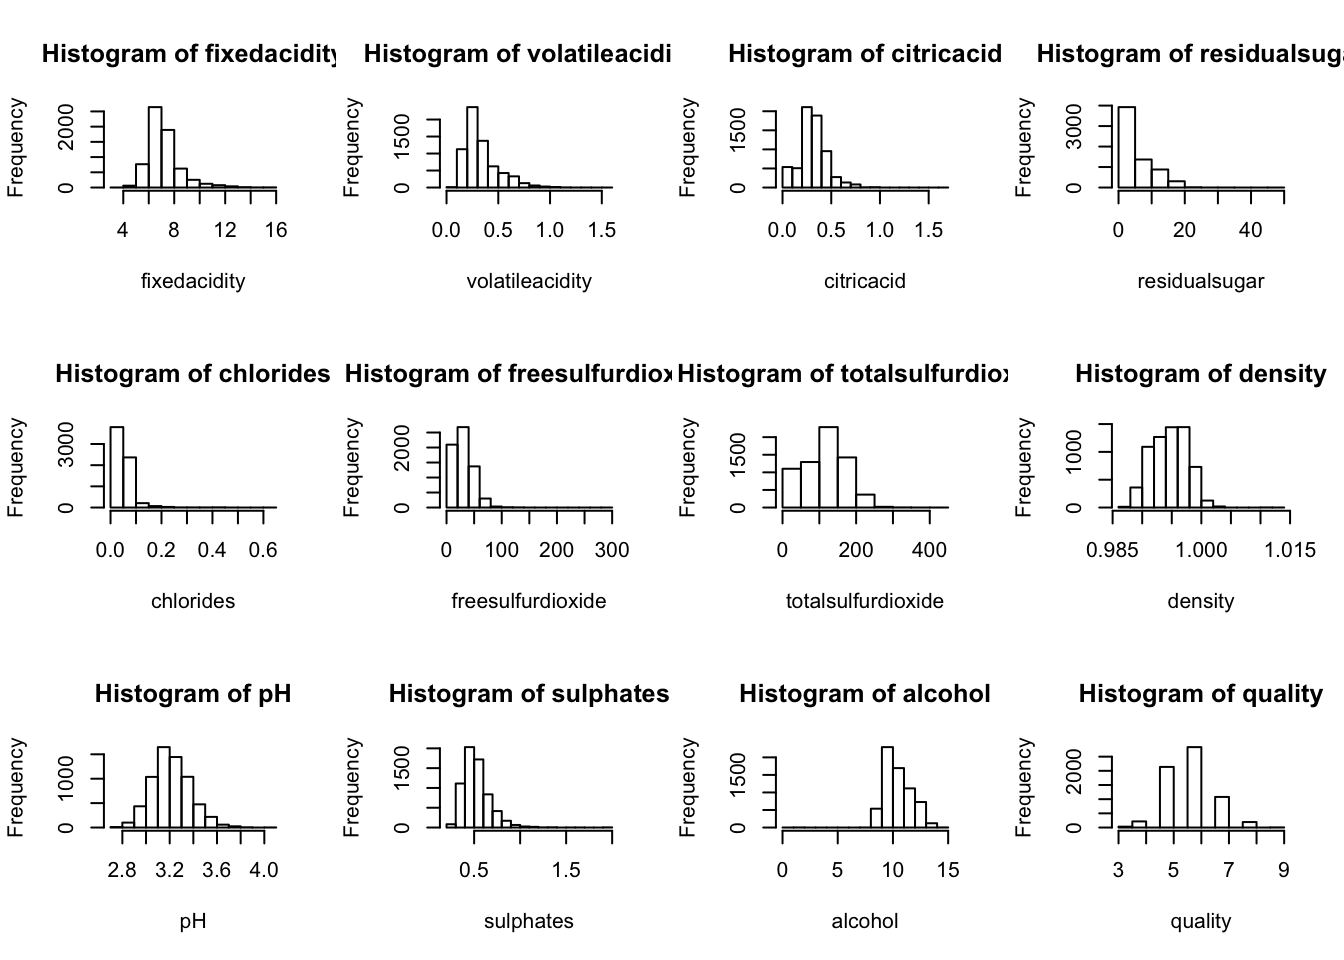
\includegraphics{Trabalho_Estatistica_180908_files/figure-latex/unnamed-chunk-9-1.pdf}
Análise:

Avaliando os histogrmas, alguns pontos chamam a atenção:

\begin{itemize}
\item
  As escalas estão bem abertas, indicando a presença de Outliers,
  principalmente para: volatileacidity, citricacid, chlorides,
  freesulfurdioxide
\item
  Distribuições assimetricas, com mínimos limitados pelo valor zero, por
  exemplo: volatileacidity, residualsugar, chlorides, freesulfurdioxide
\end{itemize}

\begin{Shaded}
\begin{Highlighting}[]
\KeywordTok{hist}\NormalTok{(quality, }\DataTypeTok{col=}\KeywordTok{c}\NormalTok{(}\StringTok{"pink"}\NormalTok{), }\DataTypeTok{col.main=}\StringTok{"darkgray"}\NormalTok{, }\DataTypeTok{prob=}\NormalTok{T)}
\end{Highlighting}
\end{Shaded}

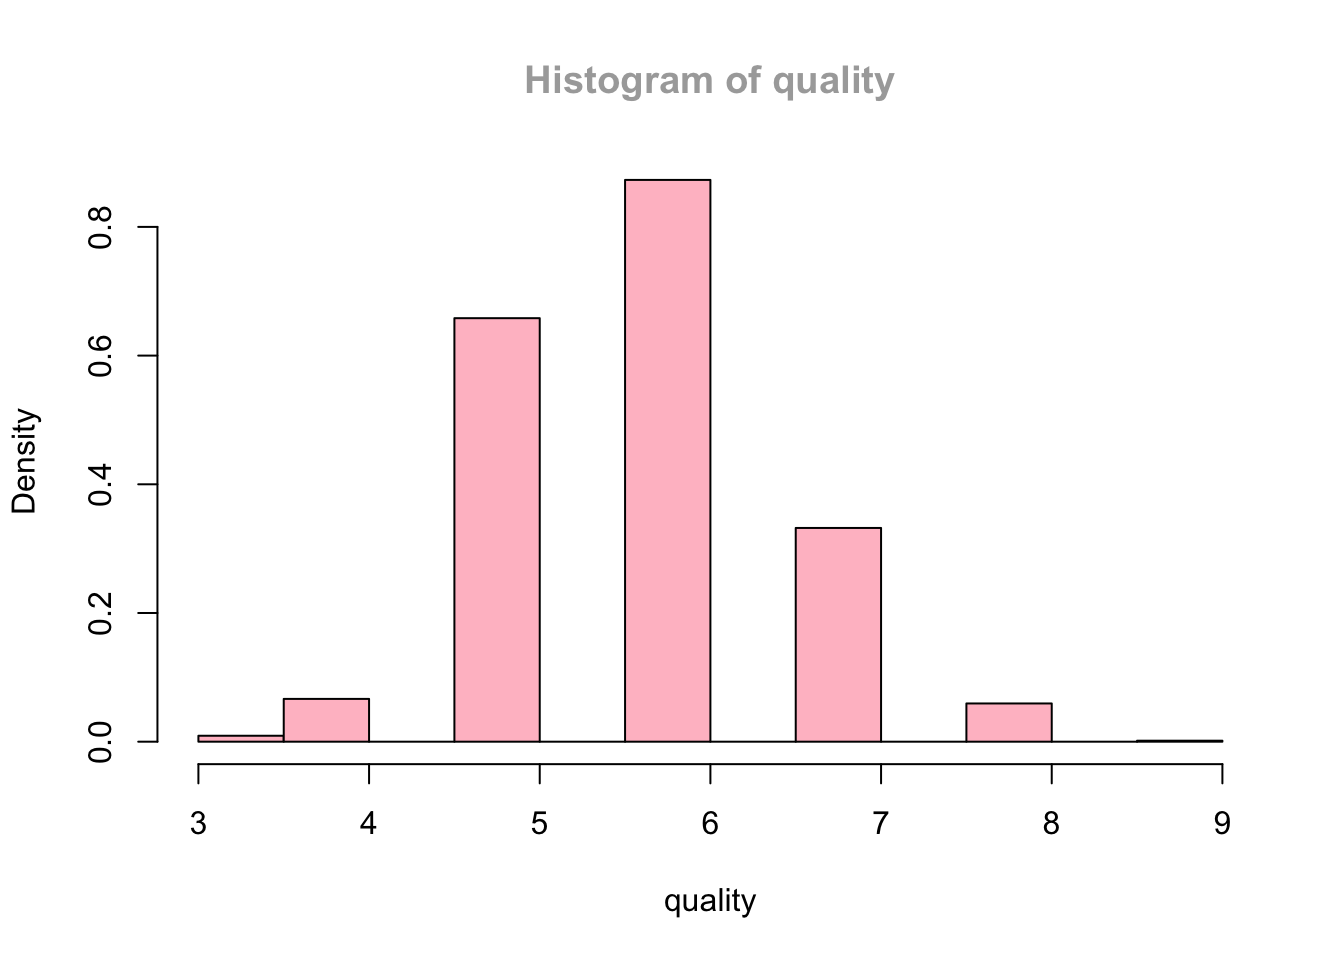
\includegraphics{Trabalho_Estatistica_180908_files/figure-latex/unnamed-chunk-10-1.pdf}
Análise:

\begin{itemize}
\tightlist
\item
  O histograma da quality, por ter valores inteiros, o histograma parece
  ``dentado'' mas que não invalida a análise de uma distribuição
  simétrica, possivelmente Normal
\end{itemize}

\begin{Shaded}
\begin{Highlighting}[]
\KeywordTok{attach}\NormalTok{(Vinhos)}
\end{Highlighting}
\end{Shaded}

\begin{verbatim}
## The following objects are masked from Vinhos (pos = 4):
## 
##     alcohol, chlorides, citricacid, density, fixedacidity,
##     freesulfurdioxide, pH, quality, residualsugar, sulphates,
##     totalsulfurdioxide, Vinho, volatileacidity
\end{verbatim}

\begin{Shaded}
\begin{Highlighting}[]
\CommentTok{#comando para gerar em 3 linhas e 4 colunas os histogramas}
\KeywordTok{par}\NormalTok{ (}\DataTypeTok{mfrow=}\KeywordTok{c}\NormalTok{(}\DecValTok{3}\NormalTok{,}\DecValTok{4}\NormalTok{))}
\KeywordTok{boxplot}\NormalTok{(fixedacidity, }\DataTypeTok{main=}\StringTok{'fixedacidity'}\NormalTok{)}
\KeywordTok{boxplot}\NormalTok{(volatileacidity , }\DataTypeTok{main=}\StringTok{'volatileacidity'}\NormalTok{)}
\KeywordTok{boxplot}\NormalTok{(citricacid , }\DataTypeTok{main=}\StringTok{'citricacid'}\NormalTok{)}
\KeywordTok{boxplot}\NormalTok{(residualsugar, }\DataTypeTok{main=}\StringTok{'residualsugar'}\NormalTok{)}
\KeywordTok{boxplot}\NormalTok{(chlorides, }\DataTypeTok{main=}\StringTok{'chlorides'}\NormalTok{)}
\KeywordTok{boxplot}\NormalTok{(freesulfurdioxide, }\DataTypeTok{main=}\StringTok{'freesulfurdioxide'}\NormalTok{)}
\KeywordTok{boxplot}\NormalTok{(totalsulfurdioxide, }\DataTypeTok{main=}\StringTok{'totalsulfurdioxide'}\NormalTok{)}
\KeywordTok{boxplot}\NormalTok{(density, }\DataTypeTok{main=}\StringTok{'density'}\NormalTok{)}
\KeywordTok{boxplot}\NormalTok{(pH, }\DataTypeTok{main=}\StringTok{'pH'}\NormalTok{)}
\KeywordTok{boxplot}\NormalTok{(sulphates, }\DataTypeTok{main=}\StringTok{'sulphates'}\NormalTok{)}
\KeywordTok{boxplot}\NormalTok{(alcohol, }\DataTypeTok{main=}\StringTok{'alcohol'}\NormalTok{)}
\KeywordTok{boxplot}\NormalTok{(Vinhos}\OperatorTok{$}\NormalTok{quality, }\DataTypeTok{main=}\StringTok{'quality'}\NormalTok{)}
\end{Highlighting}
\end{Shaded}

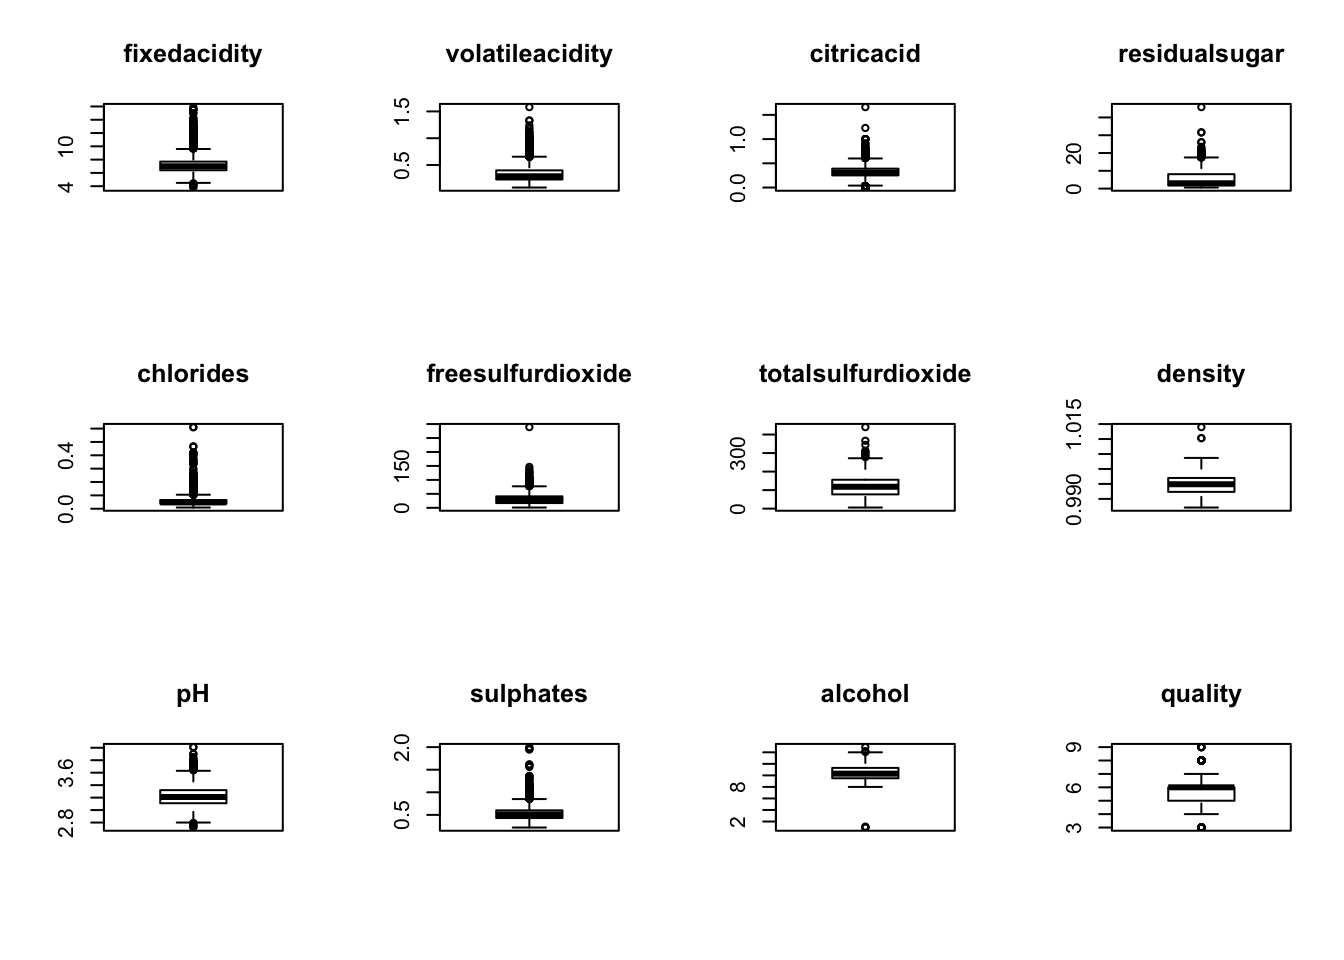
\includegraphics{Trabalho_Estatistica_180908_files/figure-latex/unnamed-chunk-11-1.pdf}
Análise:

As análises dos Box Plots validam as que já fizemos para os histogramas.

Apesar de todos os Box Plots apresentarem Outliers, que pode ser efeito
dos tamanhos de amostra, os BoxPlots com maiores quantidade de outliers
são: volatileacidity, citricacid, chlorides, freesulfurdioxide.
citricacid, freesulfurdioxide e alcohol com valores pontuais bem
distantes da distribuição. Valeria uma melhor avaliação destes pontos de
medidas para verificação se realmente são pontos fora da curva esperada.

Distribuições assimetricas, com principal atenção para residualsugar,
onde a assimentria se destaca na forma da caixa de dos bigodes do Box
Plot. Mediana deslocada para o Q1 e bigode inferior bem menor que o
superior.

\begin{Shaded}
\begin{Highlighting}[]
\KeywordTok{boxplot}\NormalTok{(quality }\OperatorTok{~}\StringTok{ }\NormalTok{Vinho, }\DataTypeTok{main=}\StringTok{'quality'}\NormalTok{)}
\end{Highlighting}
\end{Shaded}

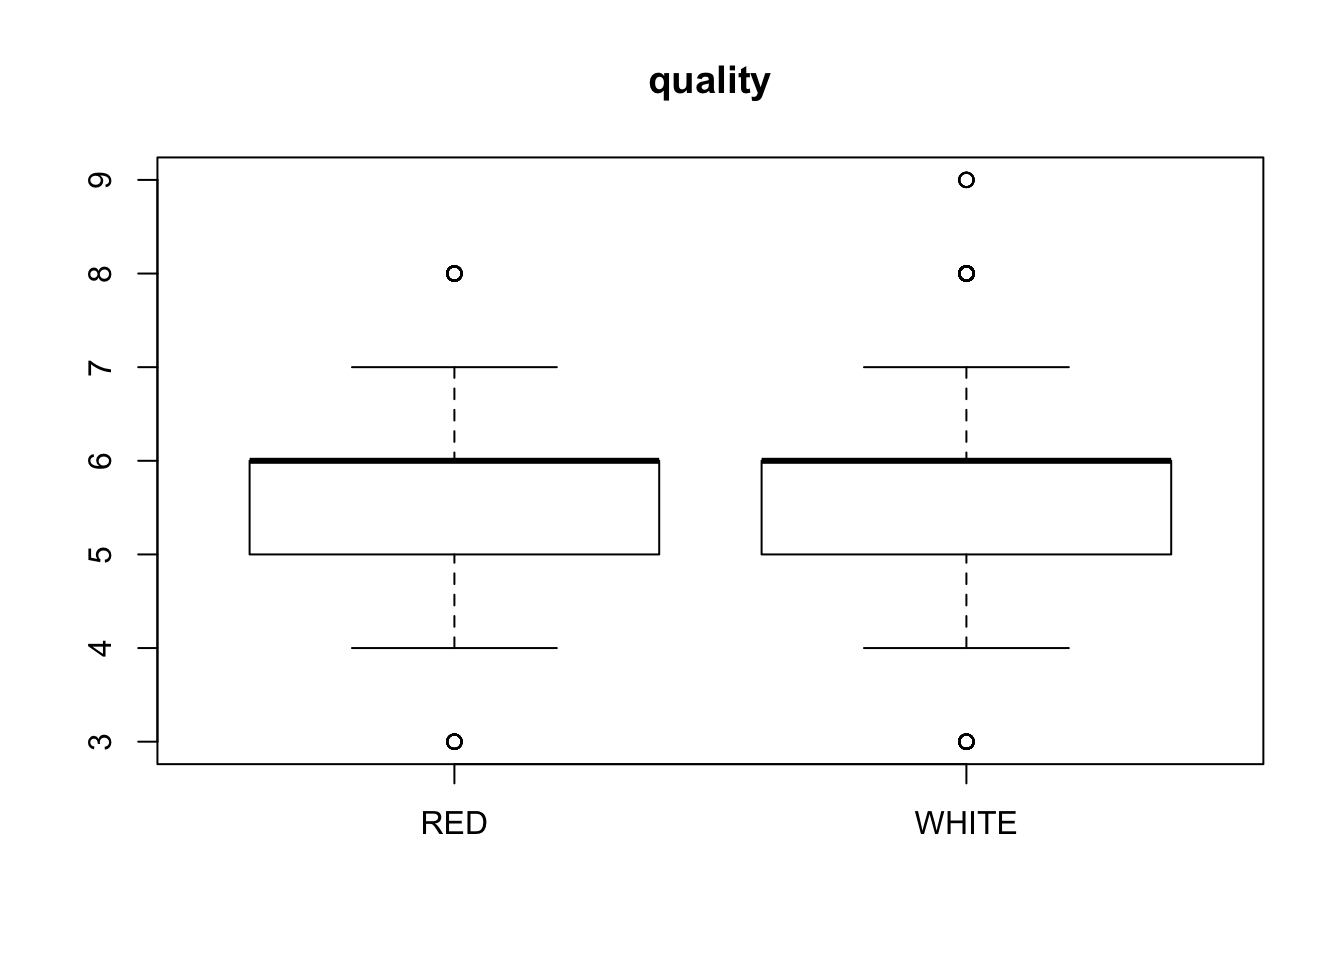
\includegraphics{Trabalho_Estatistica_180908_files/figure-latex/unnamed-chunk-12-1.pdf}

\begin{Shaded}
\begin{Highlighting}[]
\KeywordTok{boxplot}\NormalTok{(fixedacidity }\OperatorTok{~}\StringTok{ }\NormalTok{Vinho, }\DataTypeTok{main=}\StringTok{'fixedacidity'}\NormalTok{,}\DataTypeTok{col=}\KeywordTok{c}\NormalTok{(}\StringTok{'red'}\NormalTok{,}\StringTok{'blue'}\NormalTok{))}
\end{Highlighting}
\end{Shaded}

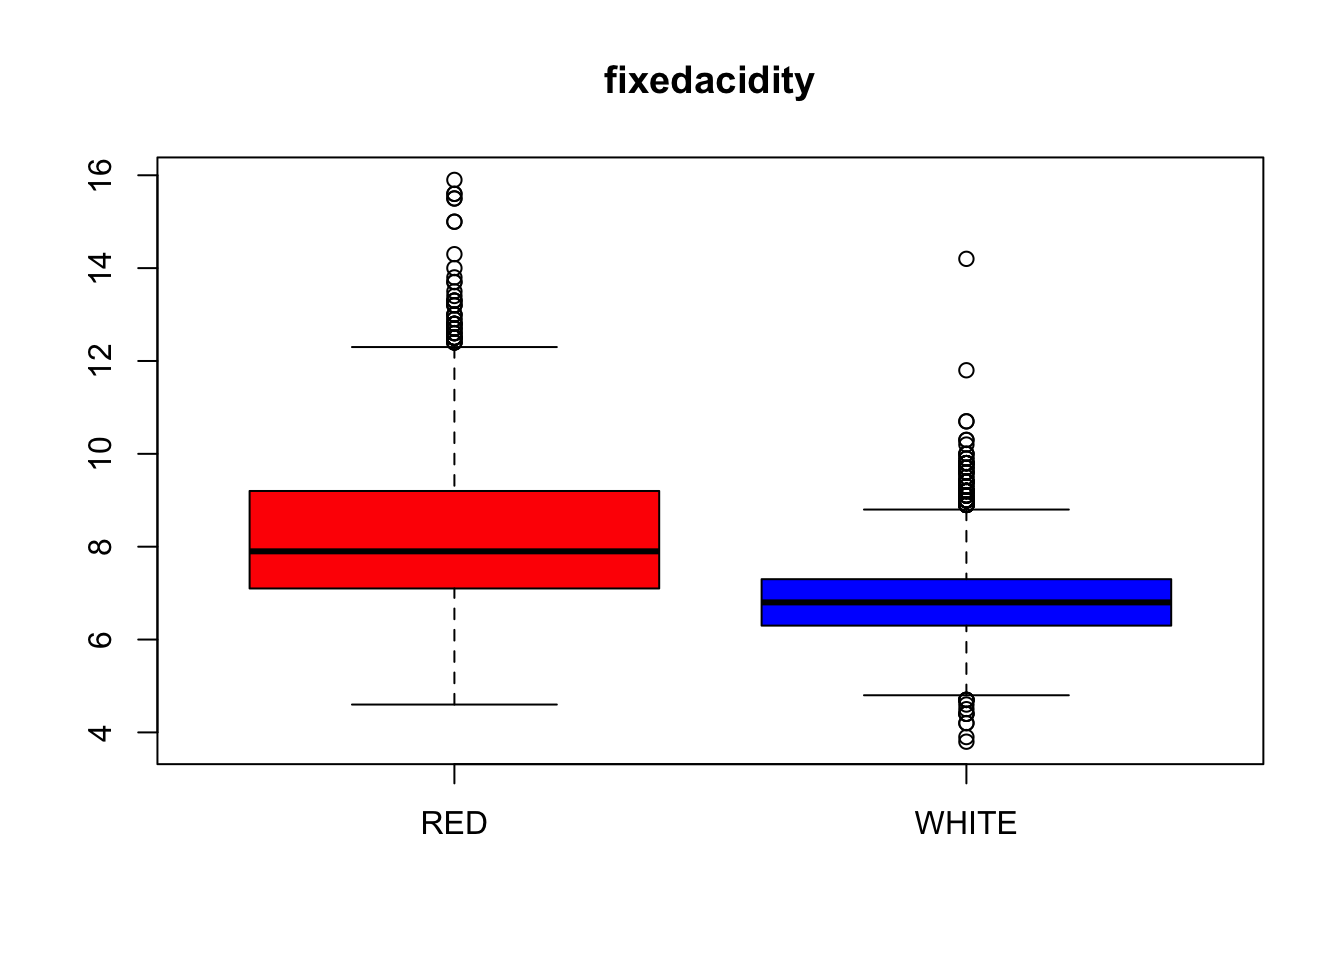
\includegraphics{Trabalho_Estatistica_180908_files/figure-latex/unnamed-chunk-12-2.pdf}

\begin{Shaded}
\begin{Highlighting}[]
\KeywordTok{boxplot}\NormalTok{(volatileacidity }\OperatorTok{~}\StringTok{ }\NormalTok{Vinho , }\DataTypeTok{main=}\StringTok{'volatileacidity'}\NormalTok{)}
\end{Highlighting}
\end{Shaded}

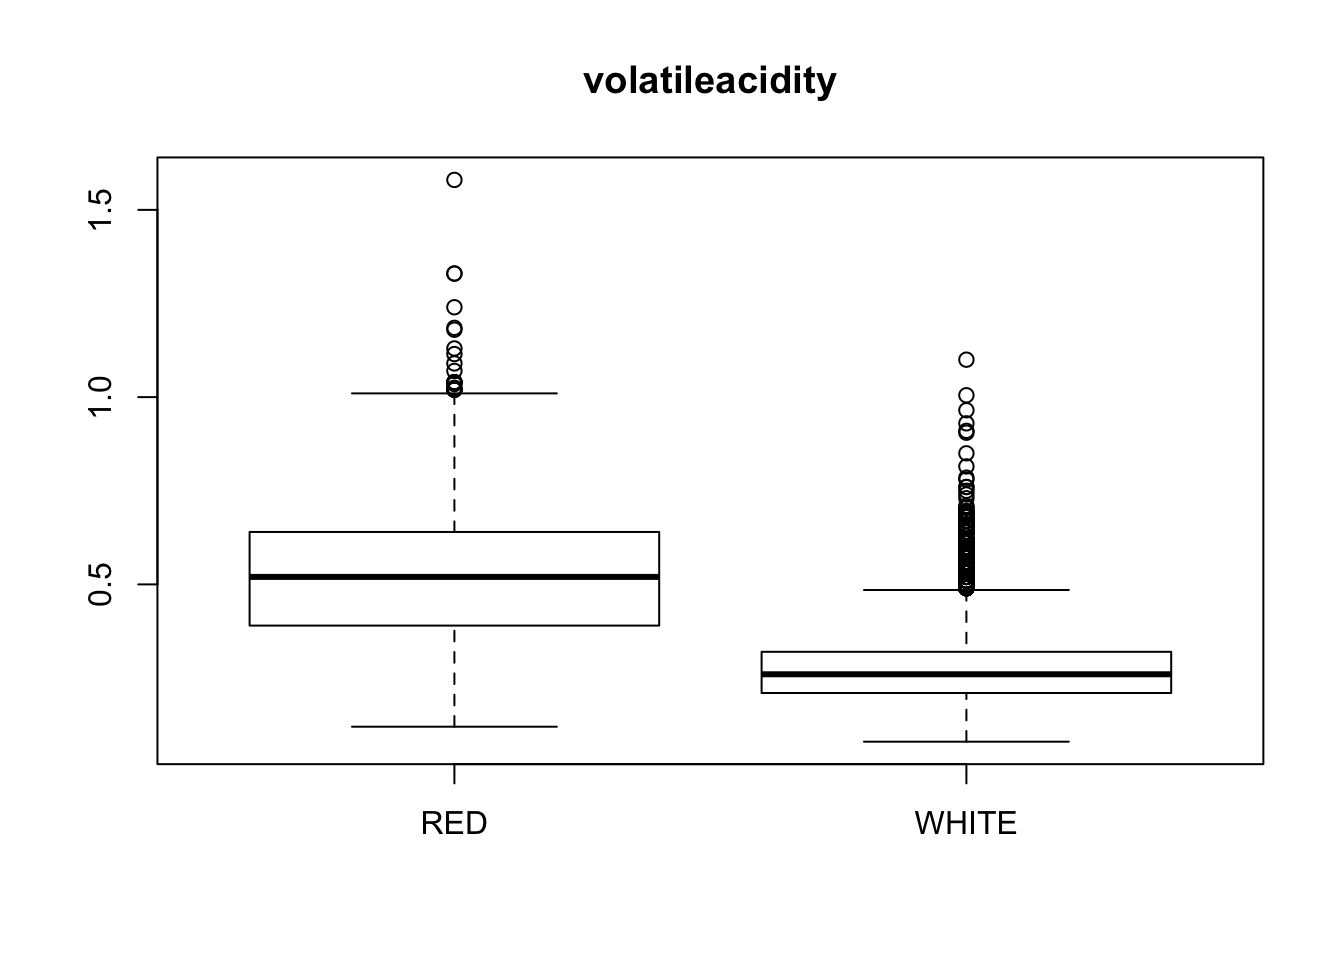
\includegraphics{Trabalho_Estatistica_180908_files/figure-latex/unnamed-chunk-12-3.pdf}

\begin{Shaded}
\begin{Highlighting}[]
\KeywordTok{boxplot}\NormalTok{(citricacid }\OperatorTok{~}\StringTok{ }\NormalTok{Vinho, }\DataTypeTok{main=}\StringTok{'citricacid'}\NormalTok{)}
\end{Highlighting}
\end{Shaded}

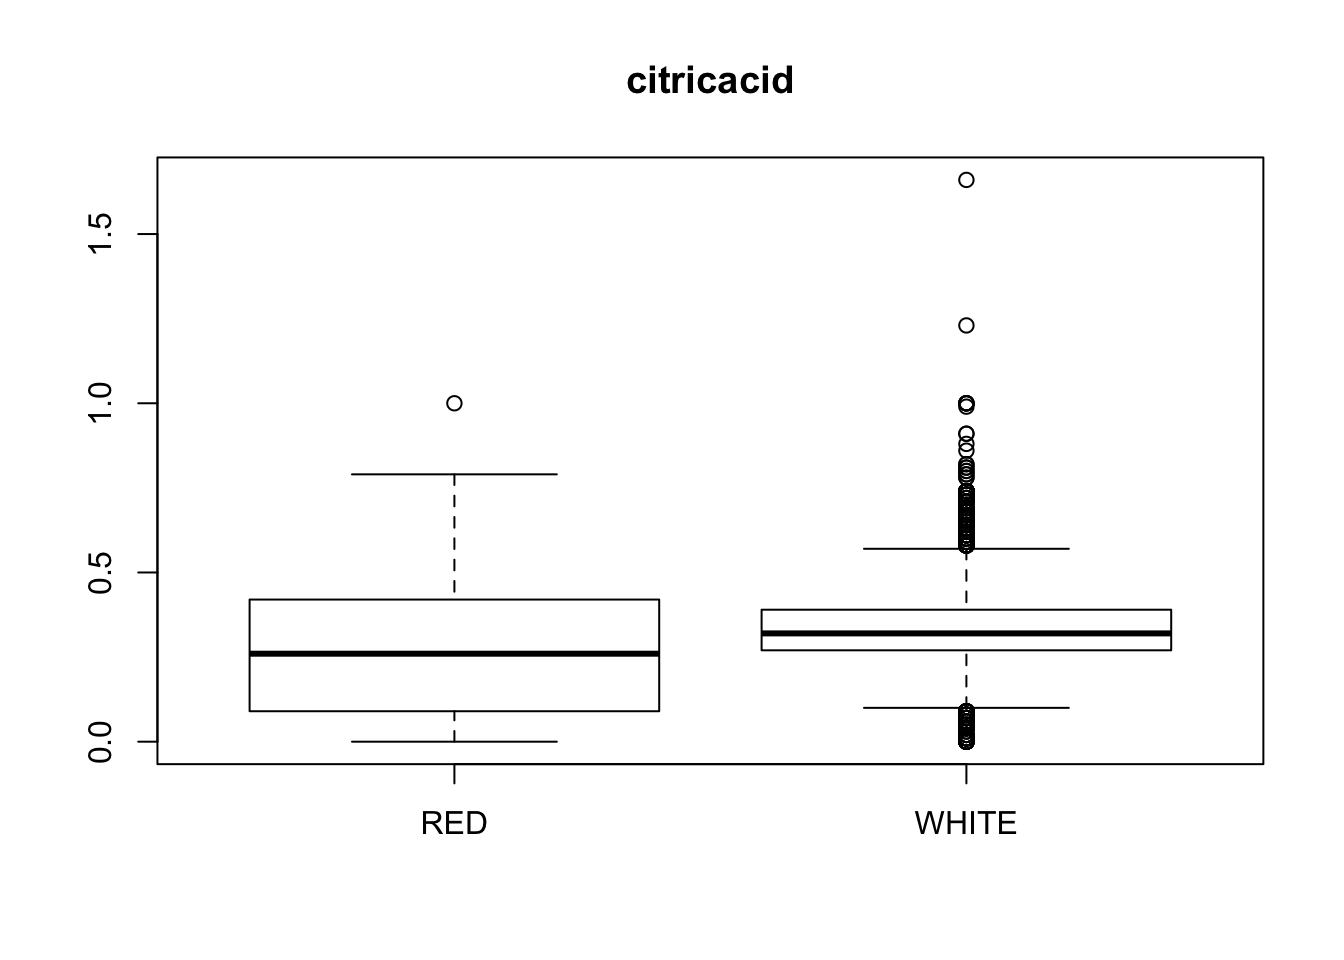
\includegraphics{Trabalho_Estatistica_180908_files/figure-latex/unnamed-chunk-12-4.pdf}

\begin{Shaded}
\begin{Highlighting}[]
\KeywordTok{boxplot}\NormalTok{(residualsugar }\OperatorTok{~}\StringTok{ }\NormalTok{Vinho, }\DataTypeTok{main=}\StringTok{'residualsugar'}\NormalTok{,}\DataTypeTok{col=}\KeywordTok{c}\NormalTok{(}\StringTok{'red'}\NormalTok{,}\StringTok{'blue'}\NormalTok{))}
\end{Highlighting}
\end{Shaded}

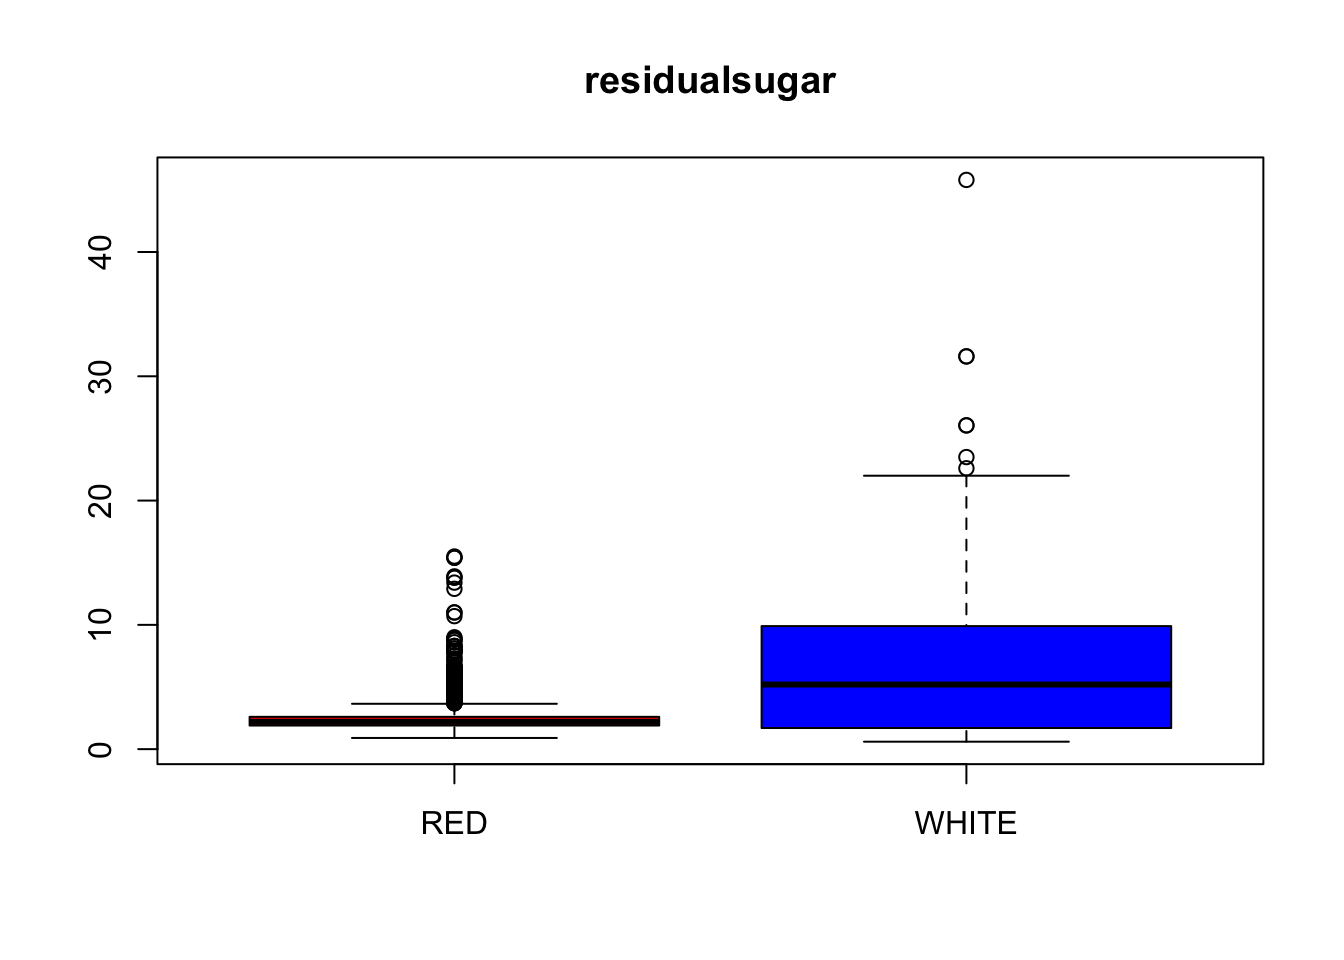
\includegraphics{Trabalho_Estatistica_180908_files/figure-latex/unnamed-chunk-12-5.pdf}

\begin{Shaded}
\begin{Highlighting}[]
\KeywordTok{boxplot}\NormalTok{(chlorides }\OperatorTok{~}\StringTok{ }\NormalTok{Vinho, }\DataTypeTok{main=}\StringTok{'chlorides'}\NormalTok{)}
\end{Highlighting}
\end{Shaded}

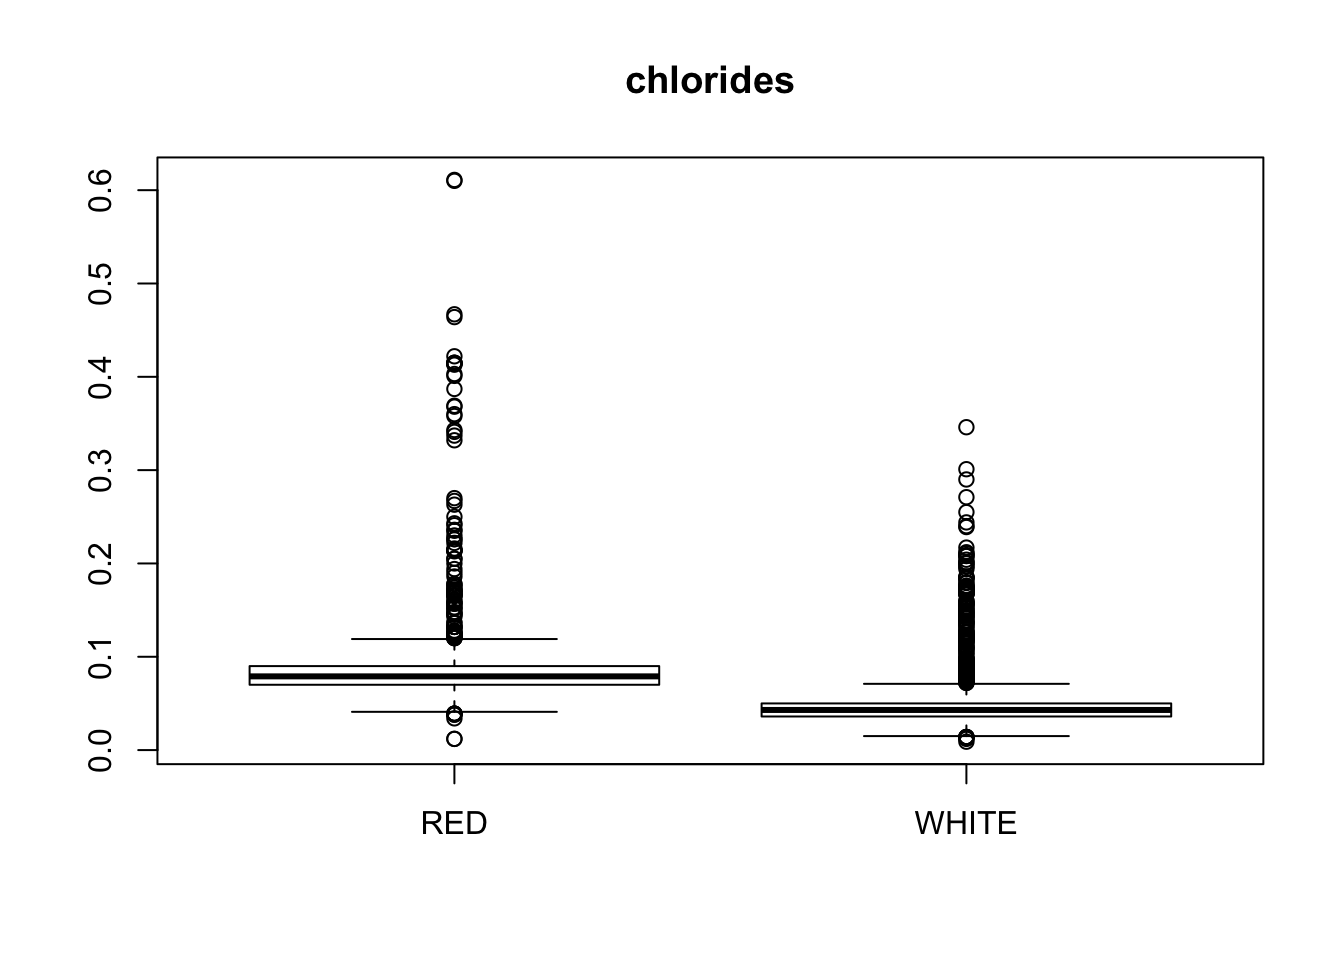
\includegraphics{Trabalho_Estatistica_180908_files/figure-latex/unnamed-chunk-12-6.pdf}

\begin{Shaded}
\begin{Highlighting}[]
\KeywordTok{boxplot}\NormalTok{(freesulfurdioxide }\OperatorTok{~}\StringTok{ }\NormalTok{Vinho, }\DataTypeTok{main=}\StringTok{'freesulfurdioxide'}\NormalTok{)}
\end{Highlighting}
\end{Shaded}

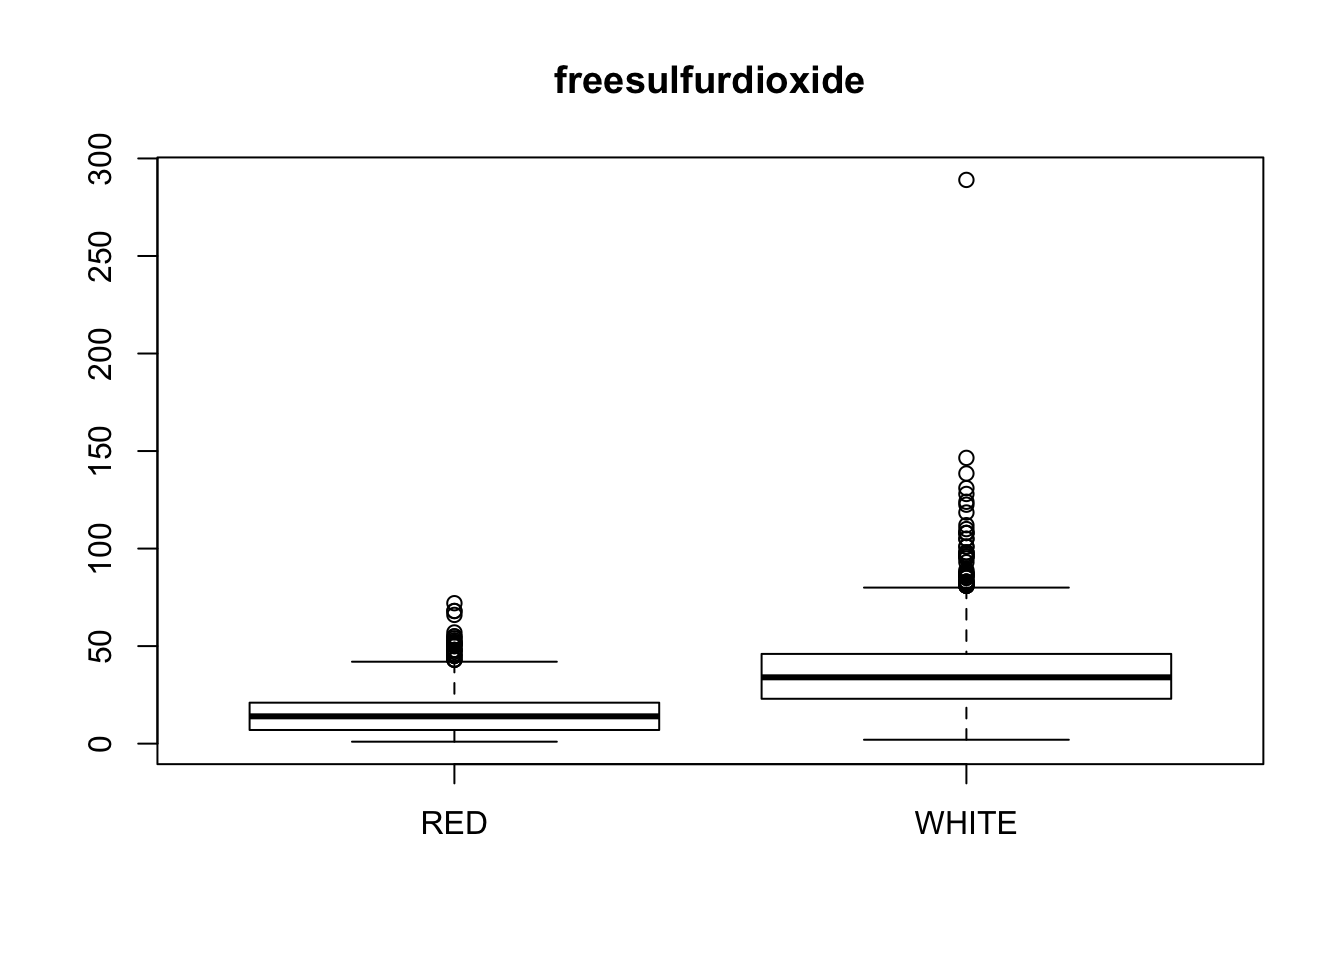
\includegraphics{Trabalho_Estatistica_180908_files/figure-latex/unnamed-chunk-12-7.pdf}

\begin{Shaded}
\begin{Highlighting}[]
\KeywordTok{boxplot}\NormalTok{(totalsulfurdioxide }\OperatorTok{~}\StringTok{ }\NormalTok{Vinho, }\DataTypeTok{main=}\StringTok{'totalsulfurdioxide'}\NormalTok{)}
\end{Highlighting}
\end{Shaded}

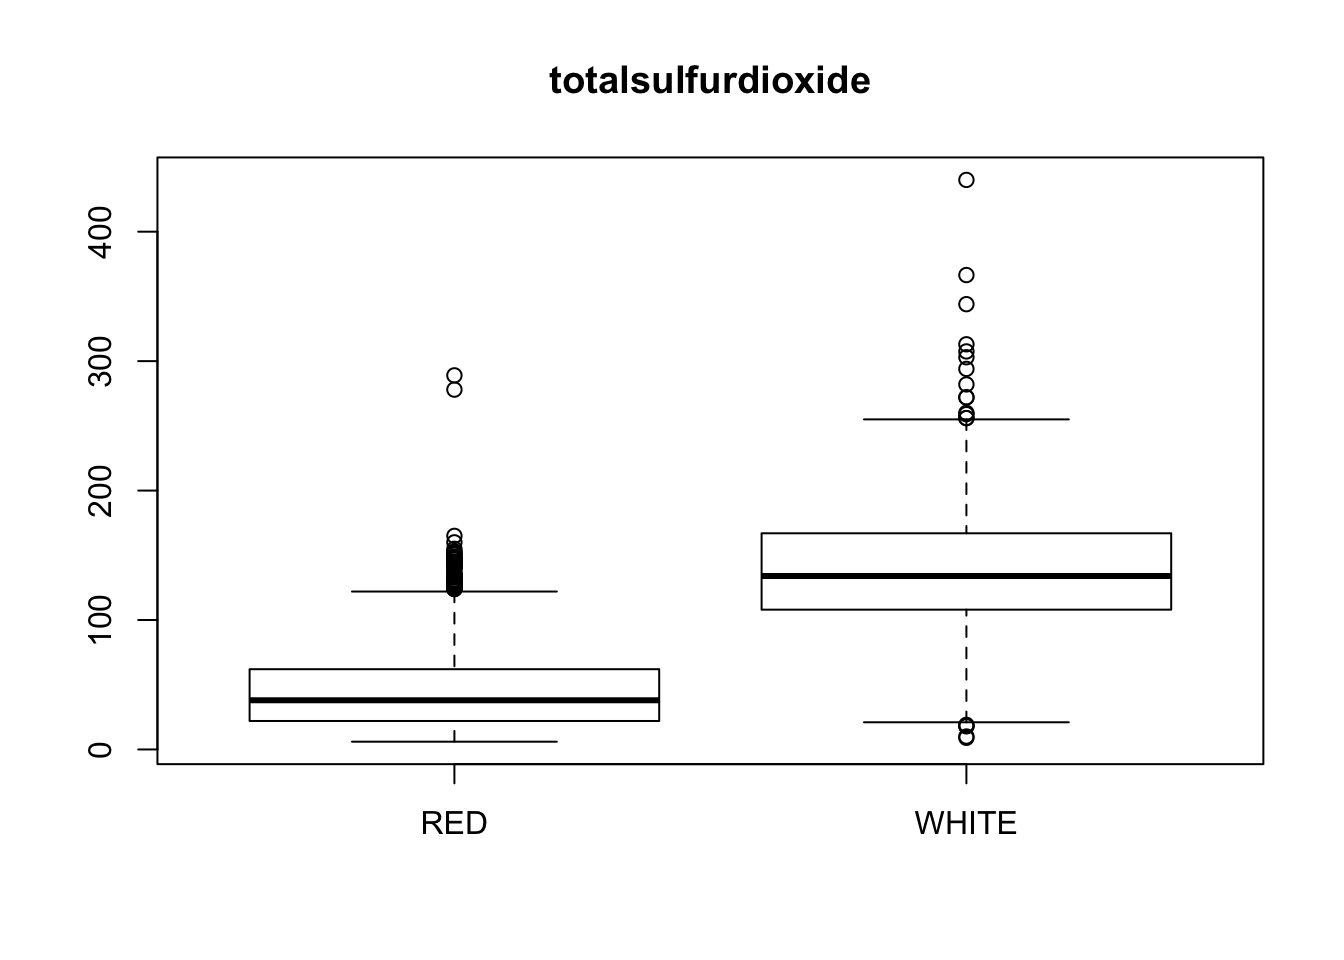
\includegraphics{Trabalho_Estatistica_180908_files/figure-latex/unnamed-chunk-12-8.pdf}

\begin{Shaded}
\begin{Highlighting}[]
\KeywordTok{boxplot}\NormalTok{(density }\OperatorTok{~}\StringTok{ }\NormalTok{Vinho, }\DataTypeTok{main=}\StringTok{'density'}\NormalTok{)}
\end{Highlighting}
\end{Shaded}

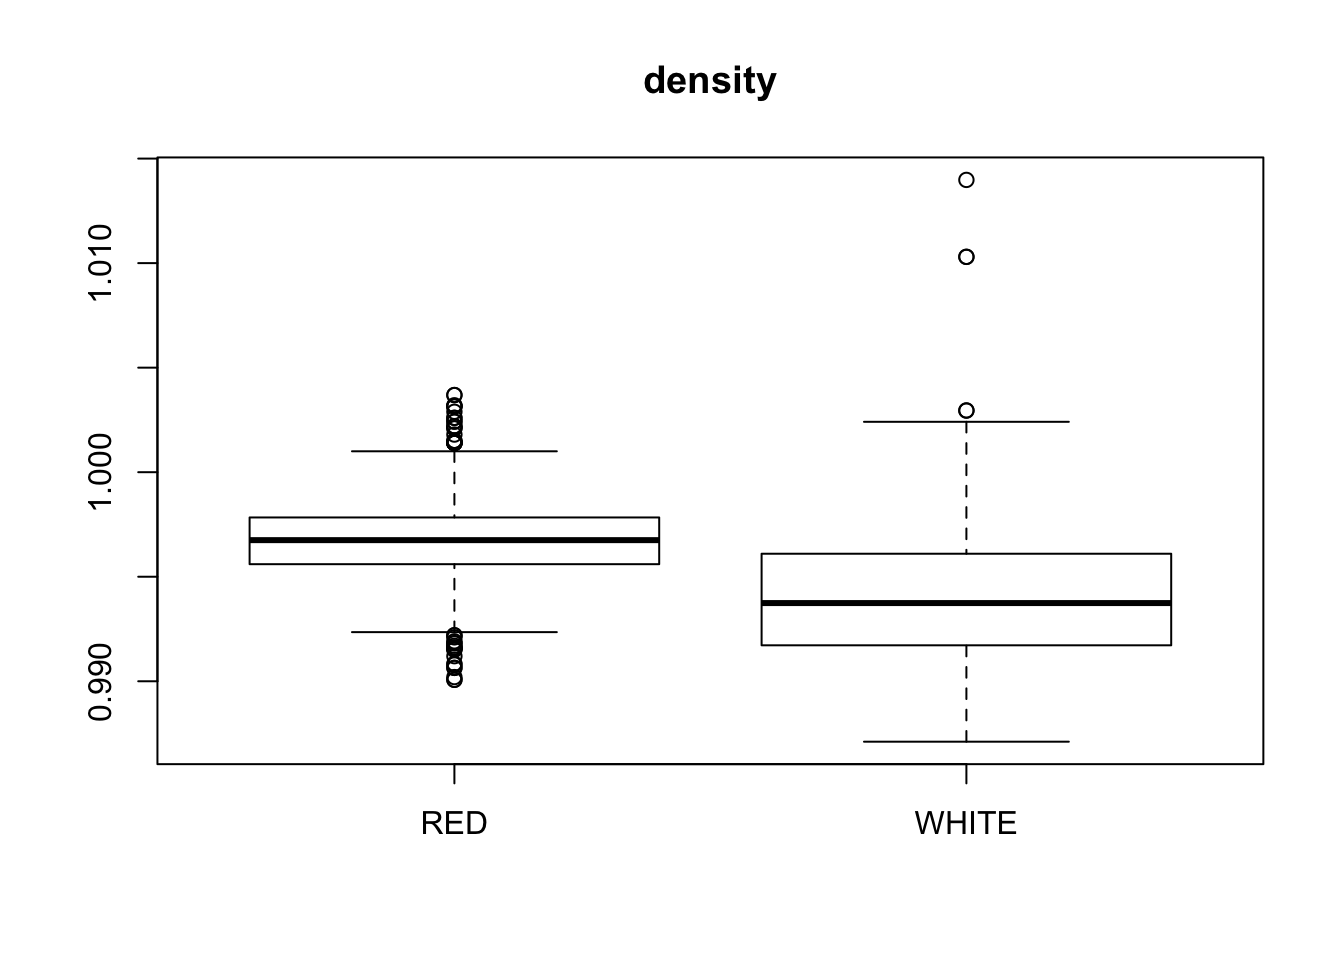
\includegraphics{Trabalho_Estatistica_180908_files/figure-latex/unnamed-chunk-12-9.pdf}

\begin{Shaded}
\begin{Highlighting}[]
\KeywordTok{boxplot}\NormalTok{(pH }\OperatorTok{~}\StringTok{ }\NormalTok{Vinho, }\DataTypeTok{main=}\StringTok{'pH'}\NormalTok{)}
\end{Highlighting}
\end{Shaded}

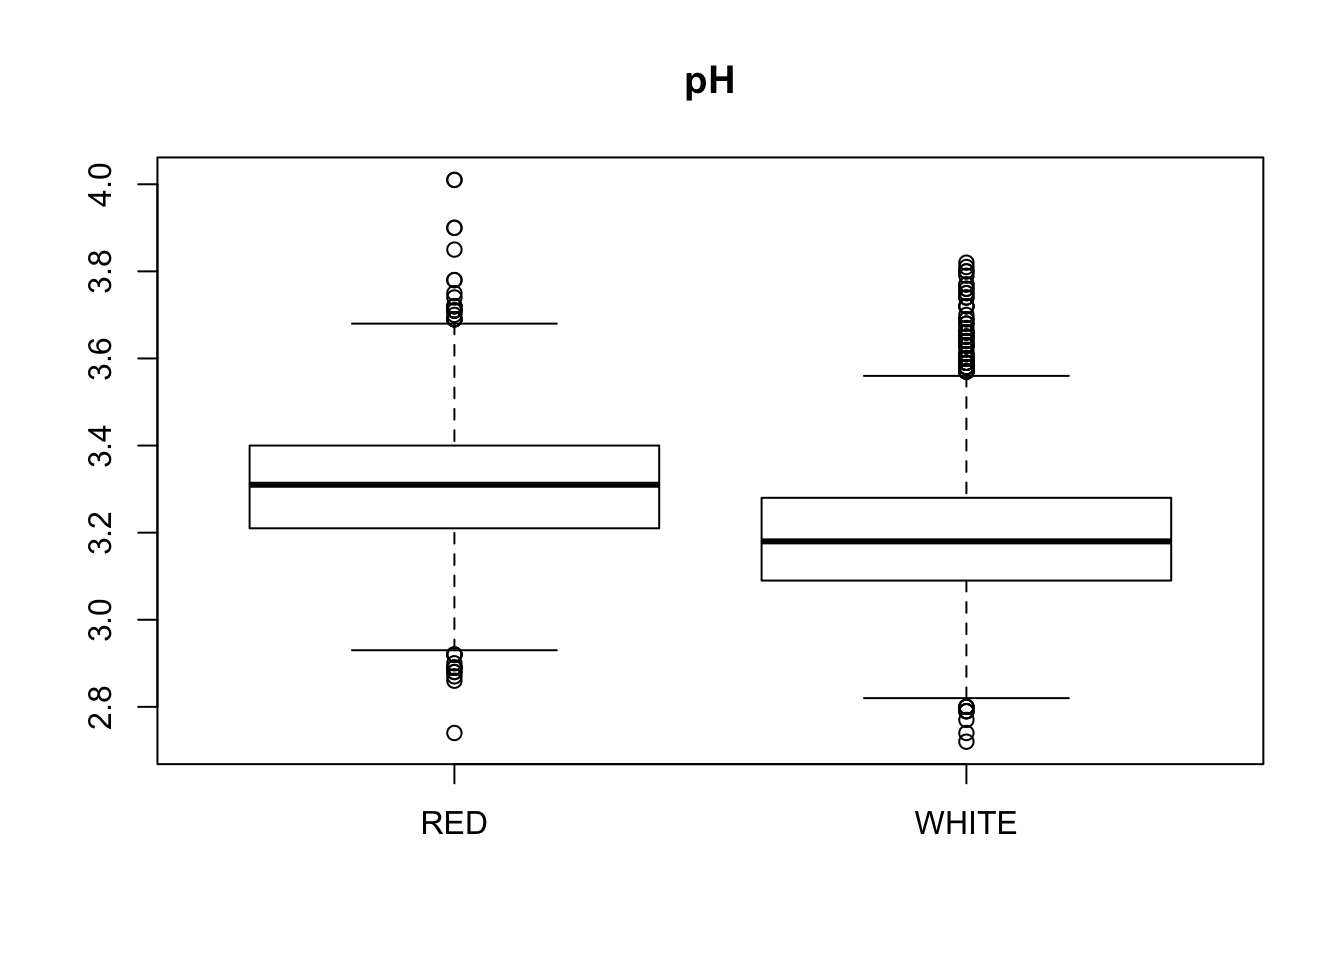
\includegraphics{Trabalho_Estatistica_180908_files/figure-latex/unnamed-chunk-12-10.pdf}

\begin{Shaded}
\begin{Highlighting}[]
\KeywordTok{boxplot}\NormalTok{(sulphates }\OperatorTok{~}\StringTok{ }\NormalTok{Vinho, }\DataTypeTok{main=}\StringTok{'sulphates'}\NormalTok{)}
\end{Highlighting}
\end{Shaded}

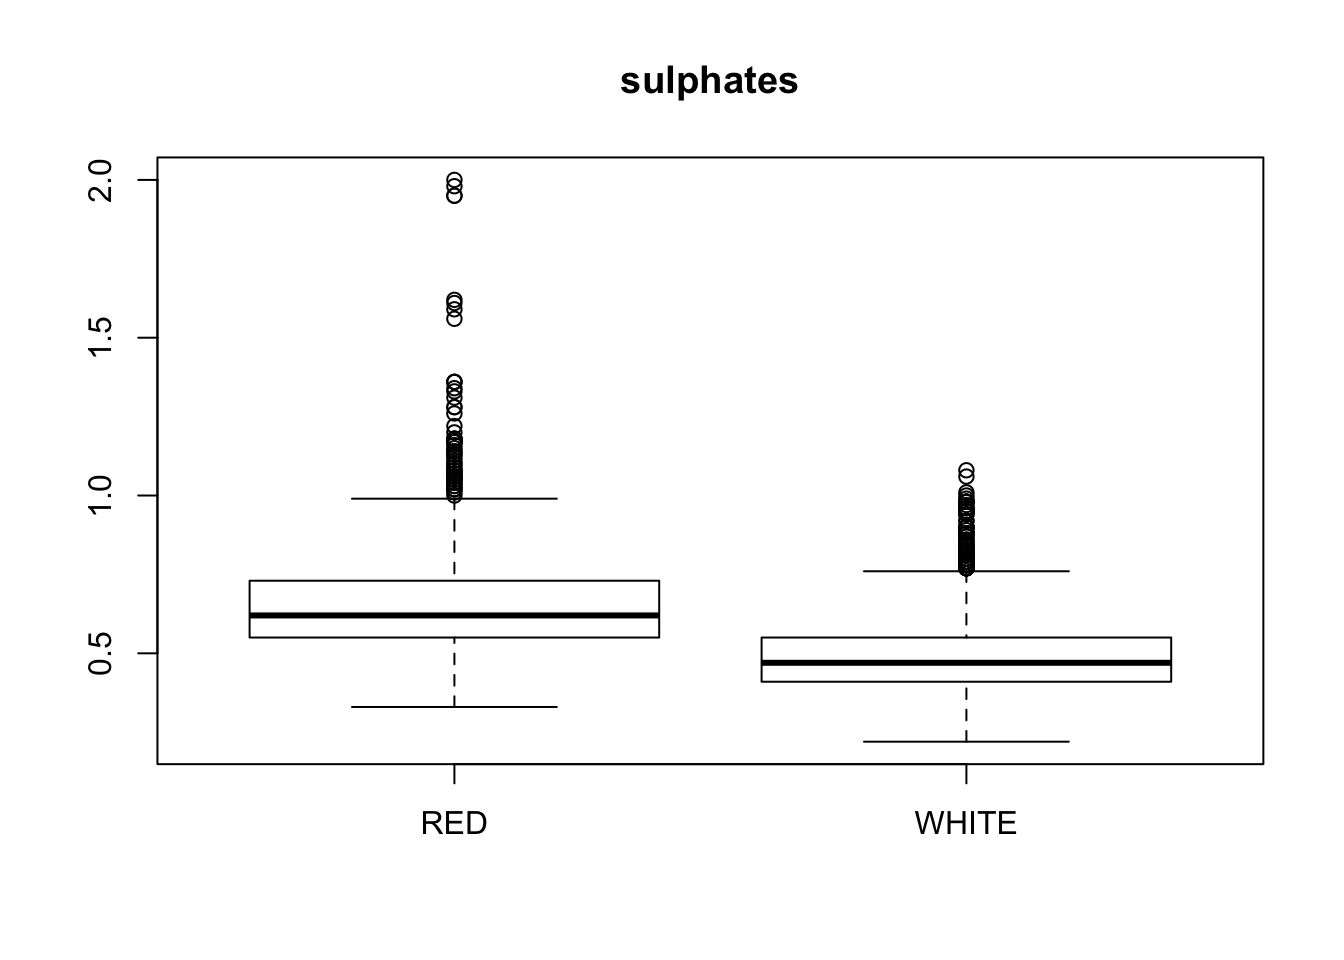
\includegraphics{Trabalho_Estatistica_180908_files/figure-latex/unnamed-chunk-12-11.pdf}

\begin{Shaded}
\begin{Highlighting}[]
\KeywordTok{boxplot}\NormalTok{(alcohol }\OperatorTok{~}\StringTok{ }\NormalTok{Vinho, }\DataTypeTok{main=}\StringTok{'alcohol'}\NormalTok{)}
\end{Highlighting}
\end{Shaded}

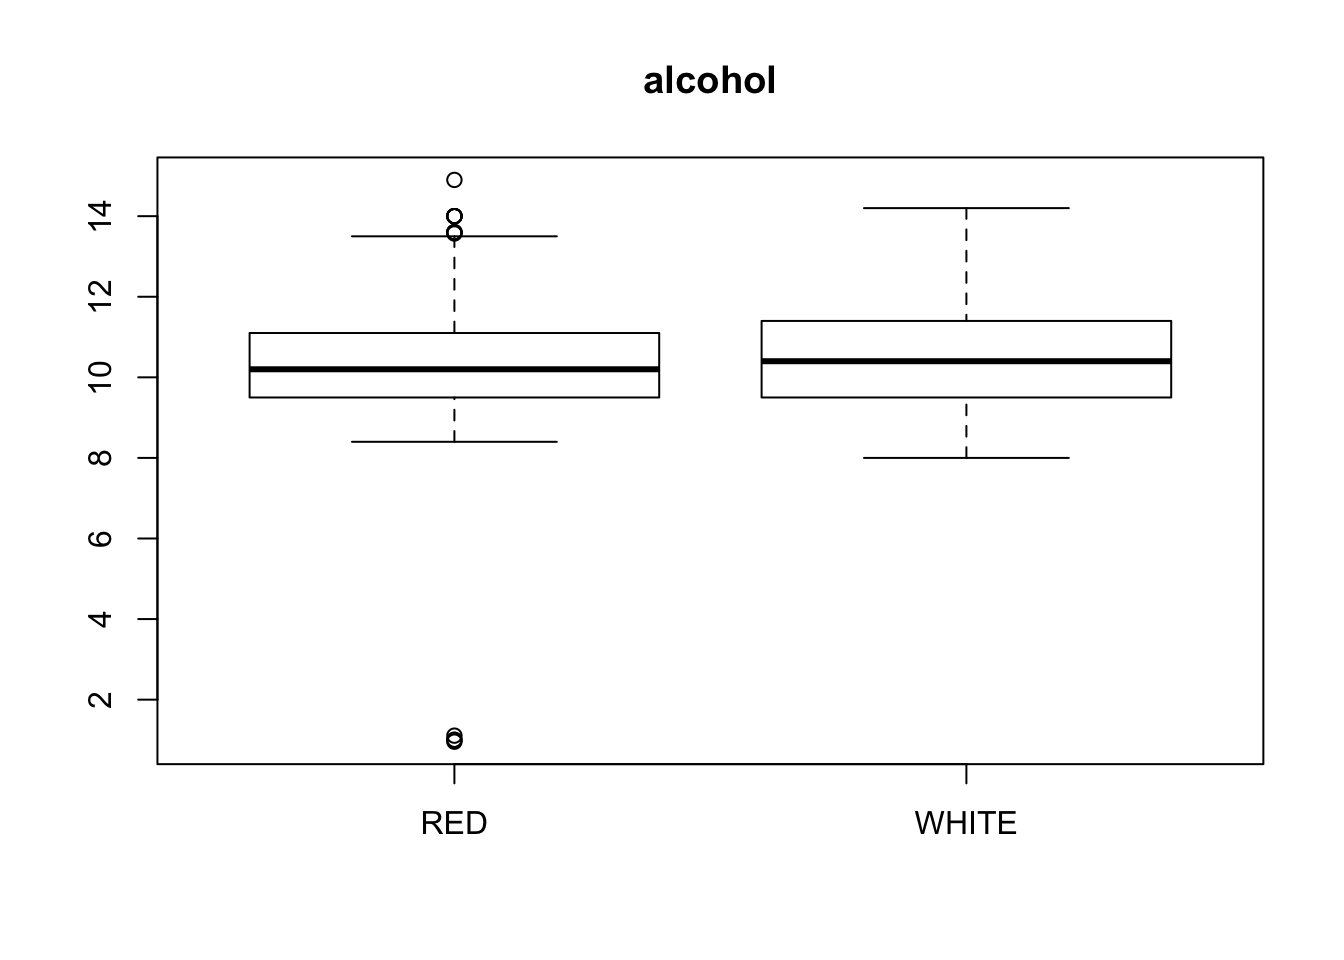
\includegraphics{Trabalho_Estatistica_180908_files/figure-latex/unnamed-chunk-12-12.pdf}
Análise:

Os Box Plots para todas as características, agora comparando os vinhos
brancos e tintos podem servir para entender características que podem
distinguir entre estes dois tipos e vinhos, como já fizemos com a
quality, usando o teste de hipótese.

Olhando os Box Plots, outras características que podem ser diferentes
por tipo de vinho são: volatileacidity, chlorides, freesulfurdioxide e
totalsulfurdioxide (já comentado nas estatísticas descritivas)

\begin{Shaded}
\begin{Highlighting}[]
\CommentTok{# Gr·fico de dispers„o ( pch=caracter, lwd=largura)}

\KeywordTok{plot}\NormalTok{(freesulfurdioxide}\OperatorTok{~}\NormalTok{totalsulfurdioxide)}
\end{Highlighting}
\end{Shaded}

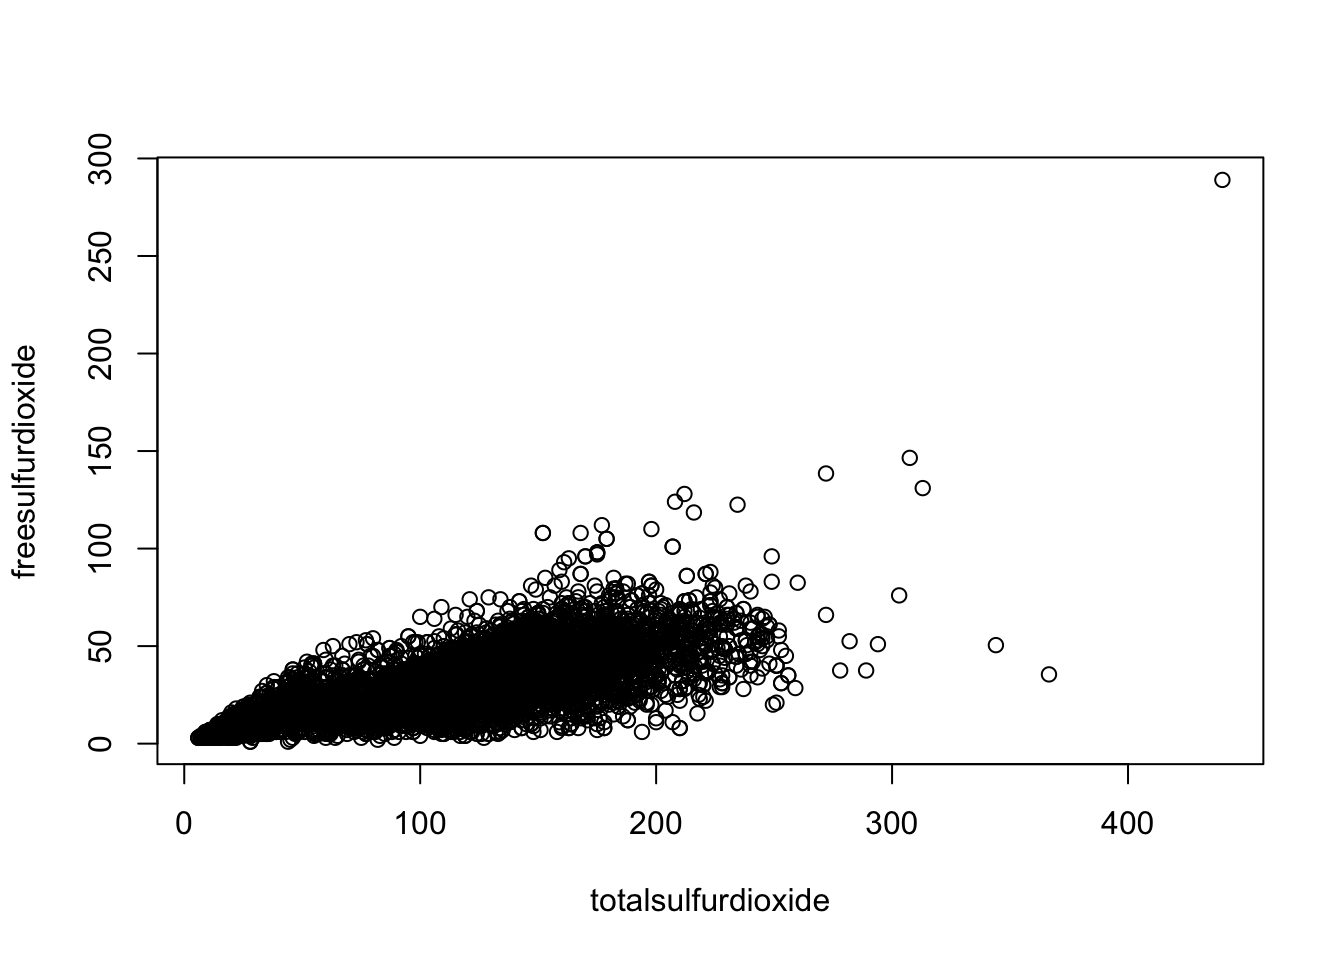
\includegraphics{Trabalho_Estatistica_180908_files/figure-latex/unnamed-chunk-13-1.pdf}

\begin{Shaded}
\begin{Highlighting}[]
\KeywordTok{plot}\NormalTok{(freesulfurdioxide}\OperatorTok{~}\NormalTok{totalsulfurdioxide, }\DataTypeTok{pch=}\DecValTok{1}\NormalTok{, }\DataTypeTok{lwd=}\DecValTok{3}\NormalTok{)}
\end{Highlighting}
\end{Shaded}

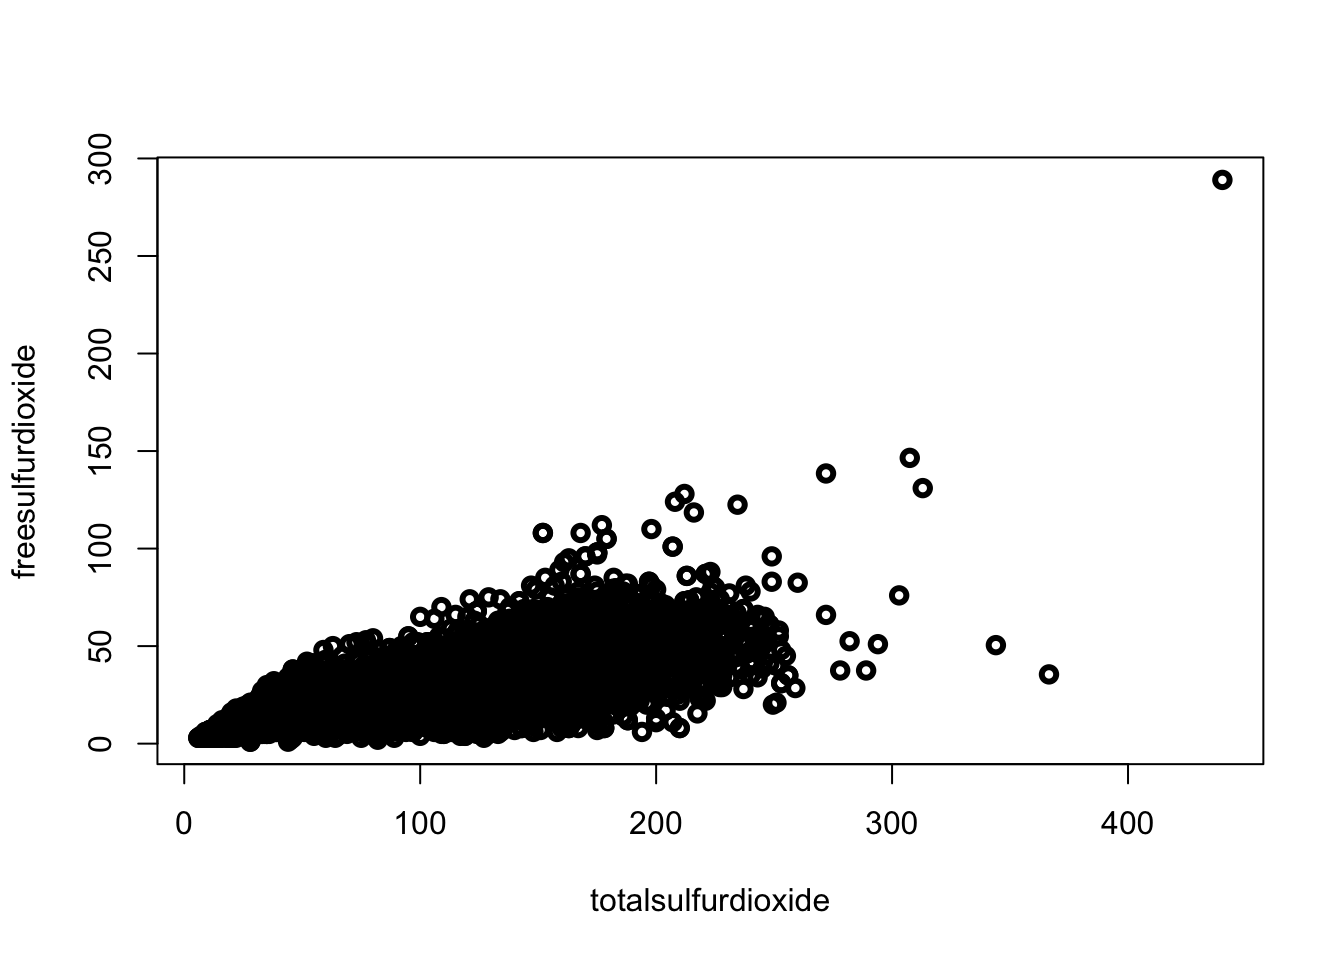
\includegraphics{Trabalho_Estatistica_180908_files/figure-latex/unnamed-chunk-13-2.pdf}

\begin{Shaded}
\begin{Highlighting}[]
\KeywordTok{plot}\NormalTok{(freesulfurdioxide}\OperatorTok{~}\NormalTok{totalsulfurdioxide)}
\KeywordTok{abline}\NormalTok{(}\DataTypeTok{h=}\KeywordTok{mean}\NormalTok{(freesulfurdioxide), }\DataTypeTok{col=}\StringTok{"red"}\NormalTok{)}
\KeywordTok{abline}\NormalTok{(}\DataTypeTok{v=}\KeywordTok{mean}\NormalTok{(totalsulfurdioxide), }\DataTypeTok{col=}\StringTok{"green"}\NormalTok{)}
\end{Highlighting}
\end{Shaded}

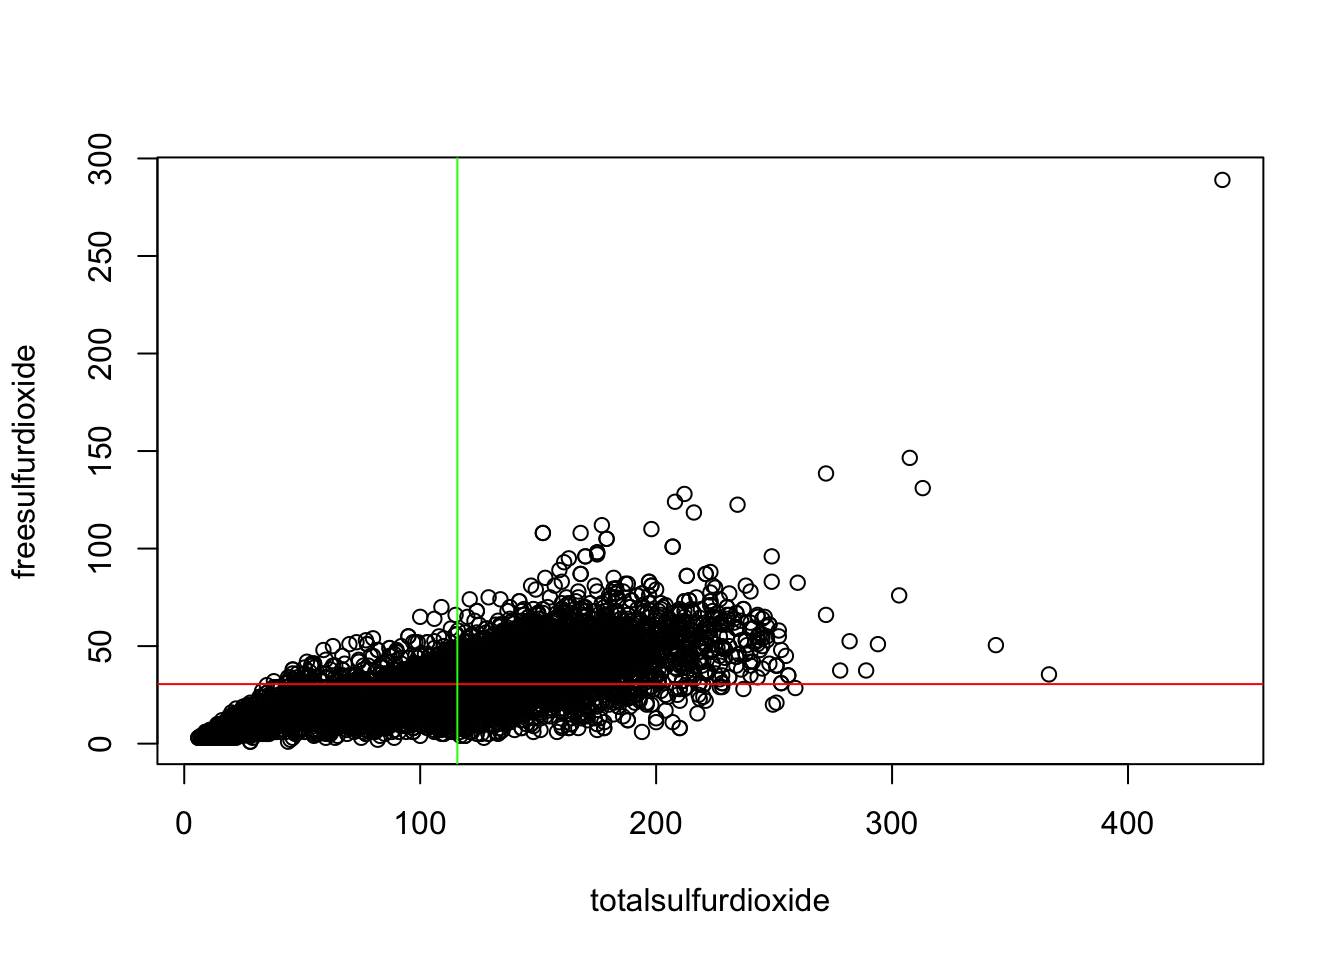
\includegraphics{Trabalho_Estatistica_180908_files/figure-latex/unnamed-chunk-13-3.pdf}
Análise:

O Gráfico de dispersão mostra a relação de previsão entre as variáveis.
Neste caso entre freesulfurdioxide e totalsulfurdioxide.

Estas variáveis aparentam ter uma correlação forte (núvem de pontos com
pouca dispersão) e positiva (inclinação positiva/coeficiente angular
\textgreater{} 0), indicando que a partir da informação sobre
totalsulfurdioxide pode prever o valor de freesulfurdioxide, com boa
acuracidade.

A linha verde representa a média do totalsulfurdioxide e a vermelha a
média do freesulfurdioxide. O ponto onde onde as retas se encontram é um
dos pontos que fará parte da regressão linear entre as variáveis e da
uma ideia de centramento desta relação

\begin{Shaded}
\begin{Highlighting}[]
\KeywordTok{attach}\NormalTok{(Vinhos)}
\end{Highlighting}
\end{Shaded}

\begin{verbatim}
## The following objects are masked from Vinhos (pos = 3):
## 
##     alcohol, chlorides, citricacid, density, fixedacidity,
##     freesulfurdioxide, pH, quality, residualsugar, sulphates,
##     totalsulfurdioxide, Vinho, volatileacidity
\end{verbatim}

\begin{verbatim}
## The following objects are masked from Vinhos (pos = 5):
## 
##     alcohol, chlorides, citricacid, density, fixedacidity,
##     freesulfurdioxide, pH, quality, residualsugar, sulphates,
##     totalsulfurdioxide, Vinho, volatileacidity
\end{verbatim}

\begin{Shaded}
\begin{Highlighting}[]
\NormalTok{Vinhos}\OperatorTok{$}\NormalTok{fx_redSugar <-}\StringTok{ }\KeywordTok{cut}\NormalTok{(residualsugar,}\DataTypeTok{breaks=}\KeywordTok{c}\NormalTok{(}\DecValTok{0}\NormalTok{,}\DecValTok{10}\NormalTok{,}\DecValTok{20}\NormalTok{,}\DecValTok{30}\NormalTok{,}\KeywordTok{max}\NormalTok{(residualsugar)))  }
\NormalTok{Vinhos}\OperatorTok{$}\NormalTok{fx_redSugar  }
\end{Highlighting}
\end{Shaded}

\begin{verbatim}
##    [1] (0,10]    (0,10]    (0,10]    (0,10]    (10,20]   (0,10]   
##    [7] (0,10]    (0,10]    (0,10]    (20,30]   (0,10]    (0,10]   
##   [13] (0,10]    (0,10]    (0,10]    (0,10]    (0,10]    (0,10]   
##   [19] (0,10]    (10,20]   (0,10]    (0,10]    (0,10]    (0,10]   
##   [25] (0,10]    (0,10]    (0,10]    (0,10]    (0,10]    (10,20]  
##   [31] (0,10]    (0,10]    (0,10]    (0,10]    (0,10]    (0,10]   
##   [37] (0,10]    (0,10]    (0,10]    (10,20]   (10,20]   (20,30]  
##   [43] (0,10]    (0,10]    (0,10]    (10,20]   (0,10]    (10,20]  
##   [49] (0,10]    (0,10]    (0,10]    (0,10]    (0,10]    (0,10]   
##   [55] (0,10]    (0,10]    (0,10]    (0,10]    (0,10]    (0,10]   
##   [61] (0,10]    (10,20]   (0,10]    (0,10]    (0,10]    (0,10]   
##   [67] (0,10]    (0,10]    (0,10]    (10,20]   (0,10]    (0,10]   
##   [73] (10,20]   (0,10]    (0,10]    (0,10]    (0,10]    (0,10]   
##   [79] (0,10]    (10,20]   (0,10]    (0,10]    (0,10]    (0,10]   
##   [85] (0,10]    (0,10]    (0,10]    (0,10]    (0,10]    (0,10]   
##   [91] (0,10]    (0,10]    (0,10]    (0,10]    (10,20]   (0,10]   
##   [97] (10,20]   (0,10]    (0,10]    (0,10]    (0,10]    (0,10]   
##  [103] (0,10]    (0,10]    (0,10]    (0,10]    (10,20]   (0,10]   
##  [109] (0,10]    (0,10]    (10,20]   (0,10]    (0,10]    (0,10]   
##  [115] (0,10]    (10,20]   (0,10]    (0,10]    (0,10]    (0,10]   
##  [121] (0,10]    (0,10]    (0,10]    (10,20]   (0,10]    (10,20]  
##  [127] (0,10]    (0,10]    (0,10]    (0,10]    (10,20]   (0,10]   
##  [133] (0,10]    (0,10]    (10,20]   (0,10]    (0,10]    (10,20]  
##  [139] (0,10]    (10,20]   (0,10]    (10,20]   (0,10]    (10,20]  
##  [145] (0,10]    (0,10]    (0,10]    (10,20]   (0,10]    (0,10]   
##  [151] (0,10]    (0,10]    (0,10]    (0,10]    (0,10]    (0,10]   
##  [157] (10,20]   (10,20]   (0,10]    (10,20]   (10,20]   (0,10]   
##  [163] (10,20]   (0,10]    (0,10]    (0,10]    (0,10]    (0,10]   
##  [169] (0,10]    (0,10]    (0,10]    (0,10]    (10,20]   (0,10]   
##  [175] (0,10]    (0,10]    (0,10]    (0,10]    (0,10]    (10,20]  
##  [181] (0,10]    (0,10]    (0,10]    (0,10]    (0,10]    (0,10]   
##  [187] (10,20]   (0,10]    (0,10]    (0,10]    (0,10]    (0,10]   
##  [193] (10,20]   (0,10]    (0,10]    (0,10]    (0,10]    (10,20]  
##  [199] (0,10]    (10,20]   (0,10]    (0,10]    (0,10]    (0,10]   
##  [205] (10,20]   (0,10]    (10,20]   (0,10]    (0,10]    (10,20]  
##  [211] (0,10]    (0,10]    (0,10]    (0,10]    (0,10]    (0,10]   
##  [217] (10,20]   (0,10]    (0,10]    (20,30]   (10,20]   (10,20]  
##  [223] (0,10]    (0,10]    (10,20]   (0,10]    (0,10]    (0,10]   
##  [229] (0,10]    (10,20]   (0,10]    (0,10]    (0,10]    (10,20]  
##  [235] (0,10]    (0,10]    (10,20]   (0,10]    (0,10]    (10,20]  
##  [241] (0,10]    (0,10]    (0,10]    (10,20]   (0,10]    (0,10]   
##  [247] (0,10]    (0,10]    (10,20]   (0,10]    (0,10]    (0,10]   
##  [253] (0,10]    (0,10]    (0,10]    (10,20]   (0,10]    (10,20]  
##  [259] (10,20]   (0,10]    (10,20]   (0,10]    (0,10]    (0,10]   
##  [265] (0,10]    (0,10]    (0,10]    (0,10]    (0,10]    (0,10]   
##  [271] (0,10]    (0,10]    (10,20]   (10,20]   (0,10]    (0,10]   
##  [277] (0,10]    (0,10]    (0,10]    (0,10]    (0,10]    (0,10]   
##  [283] (0,10]    (0,10]    (0,10]    (0,10]    (0,10]    (0,10]   
##  [289] (10,20]   (10,20]   (10,20]   (0,10]    (0,10]    (0,10]   
##  [295] (0,10]    (0,10]    (0,10]    (10,20]   (0,10]    (0,10]   
##  [301] (0,10]    (10,20]   (0,10]    (0,10]    (0,10]    (10,20]  
##  [307] (0,10]    (0,10]    (0,10]    (0,10]    (0,10]    (0,10]   
##  [313] (0,10]    (0,10]    (0,10]    (10,20]   (0,10]    (0,10]   
##  [319] (0,10]    (0,10]    (0,10]    (0,10]    (0,10]    (10,20]  
##  [325] (0,10]    (0,10]    (0,10]    (0,10]    (0,10]    (10,20]  
##  [331] (0,10]    (0,10]    (10,20]   (10,20]   (0,10]    (0,10]   
##  [337] (0,10]    (10,20]   (0,10]    (10,20]   (0,10]    (0,10]   
##  [343] (0,10]    (10,20]   (0,10]    (0,10]    (0,10]    (0,10]   
##  [349] (0,10]    (0,10]    (0,10]    (0,10]    (0,10]    (0,10]   
##  [355] (0,10]    (0,10]    (10,20]   (0,10]    (0,10]    (0,10]   
##  [361] (0,10]    (0,10]    (10,20]   (0,10]    (0,10]    (0,10]   
##  [367] (0,10]    (10,20]   (0,10]    (0,10]    (10,20]   (0,10]   
##  [373] (10,20]   (0,10]    (0,10]    (0,10]    (0,10]    (0,10]   
##  [379] (0,10]    (0,10]    (0,10]    (0,10]    (10,20]   (0,10]   
##  [385] (0,10]    (0,10]    (0,10]    (0,10]    (0,10]    (0,10]   
##  [391] (0,10]    (0,10]    (0,10]    (0,10]    (0,10]    (0,10]   
##  [397] (0,10]    (0,10]    (0,10]    (0,10]    (0,10]    (0,10]   
##  [403] (10,20]   (0,10]    (0,10]    (10,20]   (0,10]    (0,10]   
##  [409] (0,10]    (0,10]    (0,10]    (0,10]    (0,10]    (10,20]  
##  [415] (0,10]    (0,10]    (0,10]    (10,20]   (0,10]    (0,10]   
##  [421] (0,10]    (0,10]    (10,20]   (10,20]   (0,10]    (0,10]   
##  [427] (0,10]    (10,20]   (0,10]    (0,10]    (0,10]    (0,10]   
##  [433] (0,10]    (0,10]    (10,20]   (0,10]    (10,20]   (0,10]   
##  [439] (0,10]    (0,10]    (10,20]   (0,10]    (0,10]    (0,10]   
##  [445] (10,20]   (10,20]   (0,10]    (0,10]    (0,10]    (0,10]   
##  [451] (0,10]    (0,10]    (0,10]    (0,10]    (0,10]    (10,20]  
##  [457] (0,10]    (0,10]    (10,20]   (0,10]    (0,10]    (0,10]   
##  [463] (0,10]    (0,10]    (0,10]    (0,10]    (0,10]    (0,10]   
##  [469] (0,10]    (0,10]    (0,10]    (0,10]    (0,10]    (0,10]   
##  [475] (10,20]   (0,10]    (0,10]    (10,20]   (0,10]    (0,10]   
##  [481] (0,10]    (0,10]    (0,10]    (0,10]    (0,10]    (0,10]   
##  [487] (0,10]    (0,10]    (0,10]    (10,20]   (0,10]    (0,10]   
##  [493] (0,10]    (0,10]    (0,10]    (0,10]    (10,20]   (0,10]   
##  [499] (0,10]    (0,10]    (0,10]    (0,10]    (0,10]    (0,10]   
##  [505] (0,10]    (0,10]    (0,10]    (0,10]    (0,10]    (0,10]   
##  [511] (0,10]    (0,10]    (0,10]    (0,10]    (0,10]    (10,20]  
##  [517] (0,10]    (0,10]    (0,10]    (10,20]   (0,10]    (0,10]   
##  [523] (10,20]   (0,10]    (0,10]    (0,10]    (0,10]    (10,20]  
##  [529] (0,10]    (0,10]    (0,10]    (0,10]    (0,10]    (0,10]   
##  [535] (0,10]    (0,10]    (0,10]    (0,10]    (0,10]    (0,10]   
##  [541] (10,20]   (0,10]    (0,10]    (0,10]    (0,10]    (0,10]   
##  [547] (0,10]    (0,10]    (0,10]    (0,10]    (0,10]    (10,20]  
##  [553] (10,20]   (0,10]    (0,10]    (0,10]    (0,10]    (0,10]   
##  [559] (0,10]    (0,10]    (0,10]    (0,10]    (10,20]   (10,20]  
##  [565] (10,20]   (0,10]    (0,10]    (0,10]    (0,10]    (0,10]   
##  [571] (0,10]    (0,10]    (0,10]    (0,10]    (0,10]    (0,10]   
##  [577] (10,20]   (10,20]   (10,20]   (0,10]    (0,10]    (0,10]   
##  [583] (0,10]    (0,10]    (10,20]   (10,20]   (0,10]    (0,10]   
##  [589] (0,10]    (10,20]   (10,20]   (0,10]    (0,10]    (10,20]  
##  [595] (0,10]    (0,10]    (10,20]   (10,20]   (0,10]    (10,20]  
##  [601] (0,10]    (0,10]    (20,30]   (10,20]   (0,10]    (0,10]   
##  [607] (0,10]    (0,10]    (0,10]    (0,10]    (0,10]    (0,10]   
##  [613] (0,10]    (0,10]    (0,10]    (0,10]    (0,10]    (0,10]   
##  [619] (0,10]    (0,10]    (0,10]    (0,10]    (0,10]    (0,10]   
##  [625] (0,10]    (0,10]    (0,10]    (0,10]    (0,10]    (0,10]   
##  [631] (10,20]   (0,10]    (0,10]    (0,10]    (10,20]   (10,20]  
##  [637] (0,10]    (0,10]    (10,20]   (0,10]    (0,10]    (10,20]  
##  [643] (0,10]    (10,20]   (0,10]    (0,10]    (0,10]    (0,10]   
##  [649] (0,10]    (10,20]   (0,10]    (0,10]    (0,10]    (0,10]   
##  [655] (0,10]    (0,10]    (0,10]    (0,10]    (0,10]    (0,10]   
##  [661] (0,10]    (0,10]    (0,10]    (0,10]    (0,10]    (0,10]   
##  [667] (0,10]    (0,10]    (0,10]    (0,10]    (0,10]    (10,20]  
##  [673] (0,10]    (0,10]    (0,10]    (0,10]    (0,10]    (0,10]   
##  [679] (0,10]    (10,20]   (0,10]    (0,10]    (0,10]    (0,10]   
##  [685] (10,20]   (0,10]    (0,10]    (0,10]    (10,20]   (0,10]   
##  [691] (0,10]    (0,10]    (0,10]    (0,10]    (0,10]    (0,10]   
##  [697] (10,20]   (10,20]   (10,20]   (0,10]    (0,10]    (0,10]   
##  [703] (0,10]    (0,10]    (0,10]    (0,10]    (0,10]    (10,20]  
##  [709] (0,10]    (0,10]    (0,10]    (0,10]    (0,10]    (0,10]   
##  [715] (0,10]    (0,10]    (10,20]   (0,10]    (0,10]    (0,10]   
##  [721] (0,10]    (10,20]   (0,10]    (0,10]    (10,20]   (0,10]   
##  [727] (0,10]    (0,10]    (0,10]    (0,10]    (0,10]    (0,10]   
##  [733] (0,10]    (0,10]    (10,20]   (10,20]   (0,10]    (0,10]   
##  [739] (0,10]    (0,10]    (10,20]   (0,10]    (0,10]    (0,10]   
##  [745] (0,10]    (0,10]    (0,10]    (0,10]    (0,10]    (0,10]   
##  [751] (0,10]    (0,10]    (0,10]    (0,10]    (0,10]    (0,10]   
##  [757] (0,10]    (0,10]    (0,10]    (0,10]    (0,10]    (0,10]   
##  [763] (0,10]    (0,10]    (0,10]    (0,10]    (0,10]    (10,20]  
##  [769] (0,10]    (0,10]    (0,10]    (0,10]    (10,20]   (0,10]   
##  [775] (0,10]    (0,10]    (0,10]    (0,10]    (0,10]    (0,10]   
##  [781] (10,20]   (0,10]    (0,10]    (0,10]    (0,10]    (0,10]   
##  [787] (0,10]    (0,10]    (0,10]    (0,10]    (0,10]    (0,10]   
##  [793] (0,10]    (0,10]    (0,10]    (0,10]    (10,20]   (0,10]   
##  [799] (0,10]    (0,10]    (0,10]    (0,10]    (0,10]    (0,10]   
##  [805] (0,10]    (0,10]    (10,20]   (0,10]    (0,10]    (0,10]   
##  [811] (0,10]    (10,20]   (10,20]   (0,10]    (10,20]   (10,20]  
##  [817] (0,10]    (0,10]    (0,10]    (0,10]    (0,10]    (0,10]   
##  [823] (0,10]    (0,10]    (0,10]    (0,10]    (0,10]    (0,10]   
##  [829] (0,10]    (0,10]    (0,10]    (0,10]    (10,20]   (0,10]   
##  [835] (0,10]    (0,10]    (0,10]    (10,20]   (10,20]   (0,10]   
##  [841] (0,10]    (0,10]    (10,20]   (0,10]    (10,20]   (0,10]   
##  [847] (0,10]    (0,10]    (0,10]    (0,10]    (0,10]    (0,10]   
##  [853] (0,10]    (10,20]   (0,10]    (10,20]   (10,20]   (0,10]   
##  [859] (10,20]   (0,10]    (0,10]    (0,10]    (0,10]    (0,10]   
##  [865] (0,10]    (0,10]    (0,10]    (0,10]    (0,10]    (0,10]   
##  [871] (0,10]    (10,20]   (10,20]   (0,10]    (0,10]    (0,10]   
##  [877] (0,10]    (0,10]    (0,10]    (0,10]    (0,10]    (0,10]   
##  [883] (0,10]    (0,10]    (0,10]    (0,10]    (0,10]    (0,10]   
##  [889] (10,20]   (0,10]    (0,10]    (0,10]    (0,10]    (0,10]   
##  [895] (0,10]    (0,10]    (0,10]    (0,10]    (0,10]    (0,10]   
##  [901] (0,10]    (0,10]    (10,20]   (0,10]    (0,10]    (10,20]  
##  [907] (0,10]    (0,10]    (10,20]   (0,10]    (0,10]    (0,10]   
##  [913] (0,10]    (0,10]    (0,10]    (0,10]    (10,20]   (0,10]   
##  [919] (0,10]    (10,20]   (0,10]    (0,10]    (0,10]    (0,10]   
##  [925] (0,10]    (0,10]    (0,10]    (0,10]    (0,10]    (0,10]   
##  [931] (0,10]    (0,10]    (10,20]   (0,10]    (0,10]    (0,10]   
##  [937] (0,10]    (10,20]   (0,10]    (0,10]    (0,10]    (0,10]   
##  [943] (0,10]    (0,10]    (0,10]    (0,10]    (0,10]    (0,10]   
##  [949] (0,10]    (0,10]    (0,10]    (0,10]    (0,10]    (0,10]   
##  [955] (0,10]    (0,10]    (0,10]    (0,10]    (0,10]    (0,10]   
##  [961] (0,10]    (0,10]    (10,20]   (10,20]   (0,10]    (0,10]   
##  [967] (10,20]   (0,10]    (0,10]    (0,10]    (10,20]   (0,10]   
##  [973] (0,10]    (0,10]    (0,10]    (0,10]    (0,10]    (0,10]   
##  [979] (0,10]    (0,10]    (0,10]    (0,10]    (0,10]    (10,20]  
##  [985] (0,10]    (0,10]    (0,10]    (0,10]    (0,10]    (0,10]   
##  [991] (0,10]    (0,10]    (0,10]    (0,10]    (0,10]    (0,10]   
##  [997] (0,10]    (0,10]    (10,20]   (0,10]    (0,10]    (0,10]   
## [1003] (10,20]   (0,10]    (0,10]    (0,10]    (0,10]    (0,10]   
## [1009] (10,20]   (0,10]    (0,10]    (0,10]    (0,10]    (0,10]   
## [1015] (0,10]    (0,10]    (0,10]    (10,20]   (0,10]    (0,10]   
## [1021] (0,10]    (0,10]    (10,20]   (0,10]    (0,10]    (0,10]   
## [1027] (0,10]    (0,10]    (0,10]    (0,10]    (0,10]    (10,20]  
## [1033] (0,10]    (10,20]   (10,20]   (0,10]    (0,10]    (0,10]   
## [1039] (10,20]   (0,10]    (0,10]    (0,10]    (0,10]    (0,10]   
## [1045] (0,10]    (0,10]    (0,10]    (10,20]   (0,10]    (0,10]   
## [1051] (0,10]    (0,10]    (0,10]    (0,10]    (10,20]   (0,10]   
## [1057] (0,10]    (0,10]    (0,10]    (0,10]    (0,10]    (0,10]   
## [1063] (10,20]   (0,10]    (0,10]    (0,10]    (10,20]   (0,10]   
## [1069] (0,10]    (10,20]   (0,10]    (0,10]    (0,10]    (0,10]   
## [1075] (0,10]    (0,10]    (0,10]    (0,10]    (0,10]    (10,20]  
## [1081] (0,10]    (0,10]    (0,10]    (0,10]    (0,10]    (0,10]   
## [1087] (0,10]    (0,10]    (0,10]    (0,10]    (0,10]    (10,20]  
## [1093] (0,10]    (10,20]   (0,10]    (0,10]    (0,10]    (0,10]   
## [1099] (10,20]   (0,10]    (0,10]    (0,10]    (10,20]   (0,10]   
## [1105] (0,10]    (0,10]    (0,10]    (10,20]   (0,10]    (10,20]  
## [1111] (0,10]    (0,10]    (0,10]    (0,10]    (0,10]    (0,10]   
## [1117] (0,10]    (0,10]    (10,20]   (0,10]    (0,10]    (0,10]   
## [1123] (0,10]    (0,10]    (10,20]   (0,10]    (0,10]    (0,10]   
## [1129] (0,10]    (0,10]    (0,10]    (0,10]    (10,20]   (10,20]  
## [1135] (10,20]   (0,10]    (0,10]    (0,10]    (0,10]    (0,10]   
## [1141] (0,10]    (0,10]    (0,10]    (0,10]    (0,10]    (10,20]  
## [1147] (0,10]    (0,10]    (10,20]   (0,10]    (10,20]   (0,10]   
## [1153] (0,10]    (0,10]    (0,10]    (0,10]    (0,10]    (0,10]   
## [1159] (0,10]    (0,10]    (0,10]    (0,10]    (10,20]   (0,10]   
## [1165] (10,20]   (0,10]    (10,20]   (0,10]    (0,10]    (0,10]   
## [1171] (0,10]    (0,10]    (0,10]    (0,10]    (0,10]    (0,10]   
## [1177] (0,10]    (0,10]    (0,10]    (0,10]    (10,20]   (0,10]   
## [1183] (0,10]    (0,10]    (0,10]    (0,10]    (0,10]    (10,20]  
## [1189] (0,10]    (0,10]    (10,20]   (10,20]   (0,10]    (0,10]   
## [1195] (0,10]    (0,10]    (0,10]    (0,10]    (0,10]    (0,10]   
## [1201] (0,10]    (0,10]    (0,10]    (10,20]   (0,10]    (0,10]   
## [1207] (0,10]    (10,20]   (0,10]    (0,10]    (10,20]   (0,10]   
## [1213] (0,10]    (0,10]    (0,10]    (0,10]    (0,10]    (0,10]   
## [1219] (0,10]    (0,10]    (10,20]   (0,10]    (0,10]    (10,20]  
## [1225] (0,10]    (0,10]    (0,10]    (0,10]    (10,20]   (10,20]  
## [1231] (0,10]    (0,10]    (0,10]    (10,20]   (0,10]    (0,10]   
## [1237] (0,10]    (0,10]    (10,20]   (10,20]   (10,20]   (0,10]   
## [1243] (0,10]    (0,10]    (0,10]    (10,20]   (10,20]   (0,10]   
## [1249] (0,10]    (0,10]    (0,10]    (0,10]    (0,10]    (10,20]  
## [1255] (0,10]    (0,10]    (0,10]    (10,20]   (0,10]    (0,10]   
## [1261] (0,10]    (0,10]    (0,10]    (0,10]    (0,10]    (0,10]   
## [1267] (0,10]    (0,10]    (0,10]    (0,10]    (0,10]    (0,10]   
## [1273] (0,10]    (0,10]    (10,20]   (0,10]    (0,10]    (0,10]   
## [1279] (0,10]    (0,10]    (0,10]    (0,10]    (0,10]    (0,10]   
## [1285] (10,20]   (0,10]    (0,10]    (0,10]    (0,10]    (0,10]   
## [1291] (0,10]    (0,10]    (0,10]    (10,20]   (10,20]   (10,20]  
## [1297] (0,10]    (10,20]   (0,10]    (0,10]    (0,10]    (0,10]   
## [1303] (0,10]    (0,10]    (0,10]    (10,20]   (10,20]   (0,10]   
## [1309] (0,10]    (0,10]    (10,20]   (10,20]   (0,10]    (0,10]   
## [1315] (0,10]    (0,10]    (10,20]   (10,20]   (0,10]    (10,20]  
## [1321] (0,10]    (0,10]    (0,10]    (10,20]   (0,10]    (0,10]   
## [1327] (0,10]    (0,10]    (0,10]    (10,20]   (0,10]    (0,10]   
## [1333] (0,10]    (0,10]    (10,20]   (0,10]    (0,10]    (0,10]   
## [1339] (0,10]    (0,10]    (0,10]    (0,10]    (0,10]    (0,10]   
## [1345] (10,20]   (10,20]   (0,10]    (10,20]   (0,10]    (0,10]   
## [1351] (0,10]    (0,10]    (0,10]    (0,10]    (0,10]    (10,20]  
## [1357] (0,10]    (0,10]    (0,10]    (0,10]    (0,10]    (0,10]   
## [1363] (0,10]    (0,10]    (0,10]    (10,20]   (0,10]    (0,10]   
## [1369] (0,10]    (0,10]    (0,10]    (0,10]    (10,20]   (0,10]   
## [1375] (0,10]    (0,10]    (0,10]    (0,10]    (0,10]    (0,10]   
## [1381] (0,10]    (0,10]    (10,20]   (0,10]    (0,10]    (0,10]   
## [1387] (0,10]    (0,10]    (10,20]   (0,10]    (0,10]    (0,10]   
## [1393] (0,10]    (0,10]    (0,10]    (10,20]   (10,20]   (0,10]   
## [1399] (0,10]    (0,10]    (10,20]   (10,20]   (0,10]    (0,10]   
## [1405] (0,10]    (0,10]    (0,10]    (0,10]    (0,10]    (0,10]   
## [1411] (10,20]   (10,20]   (0,10]    (10,20]   (0,10]    (0,10]   
## [1417] (0,10]    (10,20]   (0,10]    (0,10]    (0,10]    (20,30]  
## [1423] (10,20]   (0,10]    (0,10]    (0,10]    (0,10]    (0,10]   
## [1429] (0,10]    (0,10]    (10,20]   (0,10]    (0,10]    (0,10]   
## [1435] (0,10]    (0,10]    (0,10]    (0,10]    (0,10]    (0,10]   
## [1441] (0,10]    (0,10]    (10,20]   (0,10]    (10,20]   (0,10]   
## [1447] (0,10]    (10,20]   (0,10]    (10,20]   (0,10]    (0,10]   
## [1453] (0,10]    (10,20]   (0,10]    (0,10]    (0,10]    (0,10]   
## [1459] (0,10]    (0,10]    (10,20]   (0,10]    (0,10]    (0,10]   
## [1465] (10,20]   (0,10]    (0,10]    (0,10]    (0,10]    (0,10]   
## [1471] (0,10]    (10,20]   (0,10]    (0,10]    (0,10]    (0,10]   
## [1477] (0,10]    (10,20]   (10,20]   (0,10]    (0,10]    (0,10]   
## [1483] (0,10]    (0,10]    (0,10]    (10,20]   (0,10]    (0,10]   
## [1489] (0,10]    (10,20]   (20,30]   (0,10]    (0,10]    (0,10]   
## [1495] (0,10]    (0,10]    (0,10]    (0,10]    (0,10]    (0,10]   
## [1501] (0,10]    (0,10]    (10,20]   (0,10]    (30,45.8] (0,10]   
## [1507] (10,20]   (0,10]    (0,10]    (0,10]    (0,10]    (0,10]   
## [1513] (10,20]   (0,10]    (10,20]   (0,10]    (0,10]    (0,10]   
## [1519] (0,10]    (0,10]    (10,20]   (0,10]    (0,10]    (0,10]   
## [1525] (10,20]   (0,10]    (0,10]    (0,10]    (0,10]    (0,10]   
## [1531] (0,10]    (0,10]    (10,20]   (10,20]   (0,10]    (0,10]   
## [1537] (0,10]    (0,10]    (0,10]    (0,10]    (0,10]    (0,10]   
## [1543] (10,20]   (0,10]    (0,10]    (10,20]   (0,10]    (0,10]   
## [1549] (0,10]    (10,20]   (0,10]    (0,10]    (0,10]    (10,20]  
## [1555] (0,10]    (0,10]    (0,10]    (0,10]    (0,10]    (0,10]   
## [1561] (0,10]    (0,10]    (0,10]    (0,10]    (0,10]    (0,10]   
## [1567] (0,10]    (0,10]    (0,10]    (0,10]    (0,10]    (0,10]   
## [1573] (10,20]   (0,10]    (0,10]    (0,10]    (0,10]    (0,10]   
## [1579] (0,10]    (10,20]   (0,10]    (0,10]    (0,10]    (0,10]   
## [1585] (10,20]   (0,10]    (10,20]   (0,10]    (0,10]    (0,10]   
## [1591] (0,10]    (0,10]    (0,10]    (0,10]    (0,10]    (10,20]  
## [1597] (10,20]   (0,10]    (0,10]    (0,10]    (0,10]    (0,10]   
## [1603] (0,10]    (0,10]    (10,20]   (10,20]   (0,10]    (0,10]   
## [1609] (0,10]    (0,10]    (0,10]    (0,10]    (10,20]   (0,10]   
## [1615] (10,20]   (0,10]    (0,10]    (10,20]   (0,10]    (0,10]   
## [1621] (0,10]    (0,10]    (0,10]    (0,10]    (0,10]    (10,20]  
## [1627] (10,20]   (0,10]    (0,10]    (10,20]   (0,10]    (0,10]   
## [1633] (0,10]    (0,10]    (0,10]    (0,10]    (0,10]    (0,10]   
## [1639] (0,10]    (10,20]   (0,10]    (0,10]    (0,10]    (0,10]   
## [1645] (0,10]    (0,10]    (0,10]    (0,10]    (0,10]    (0,10]   
## [1651] (0,10]    (0,10]    (0,10]    (0,10]    (0,10]    (0,10]   
## [1657] (0,10]    (0,10]    (0,10]    (0,10]    (0,10]    (0,10]   
## [1663] (0,10]    (0,10]    (0,10]    (0,10]    (0,10]    (10,20]  
## [1669] (0,10]    (0,10]    (10,20]   (0,10]    (0,10]    (0,10]   
## [1675] (0,10]    (0,10]    (10,20]   (0,10]    (0,10]    (10,20]  
## [1681] (0,10]    (10,20]   (0,10]    (0,10]    (0,10]    (0,10]   
## [1687] (0,10]    (0,10]    (0,10]    (0,10]    (0,10]    (0,10]   
## [1693] (0,10]    (0,10]    (0,10]    (0,10]    (10,20]   (0,10]   
## [1699] (0,10]    (0,10]    (0,10]    (0,10]    (0,10]    (0,10]   
## [1705] (0,10]    (0,10]    (0,10]    (10,20]   (0,10]    (0,10]   
## [1711] (0,10]    (0,10]    (0,10]    (0,10]    (0,10]    (0,10]   
## [1717] (0,10]    (0,10]    (0,10]    (10,20]   (0,10]    (0,10]   
## [1723] (0,10]    (0,10]    (0,10]    (0,10]    (10,20]   (0,10]   
## [1729] (0,10]    (0,10]    (10,20]   (0,10]    (10,20]   (0,10]   
## [1735] (0,10]    (10,20]   (0,10]    (0,10]    (0,10]    (0,10]   
## [1741] (0,10]    (0,10]    (0,10]    (0,10]    (0,10]    (0,10]   
## [1747] (0,10]    (0,10]    (0,10]    (0,10]    (10,20]   (0,10]   
## [1753] (10,20]   (0,10]    (0,10]    (0,10]    (0,10]    (10,20]  
## [1759] (0,10]    (0,10]    (0,10]    (0,10]    (0,10]    (0,10]   
## [1765] (0,10]    (0,10]    (10,20]   (10,20]   (0,10]    (0,10]   
## [1771] (0,10]    (0,10]    (0,10]    (0,10]    (10,20]   (0,10]   
## [1777] (0,10]    (10,20]   (0,10]    (0,10]    (0,10]    (0,10]   
## [1783] (0,10]    (10,20]   (0,10]    (0,10]    (0,10]    (10,20]  
## [1789] (0,10]    (0,10]    (0,10]    (0,10]    (10,20]   (0,10]   
## [1795] (10,20]   (10,20]   (0,10]    (0,10]    (0,10]    (0,10]   
## [1801] (0,10]    (0,10]    (0,10]    (0,10]    (0,10]    (0,10]   
## [1807] (0,10]    (0,10]    (10,20]   (0,10]    (10,20]   (0,10]   
## [1813] (0,10]    (0,10]    (0,10]    (0,10]    (10,20]   (10,20]  
## [1819] (0,10]    (0,10]    (0,10]    (0,10]    (10,20]   (0,10]   
## [1825] (0,10]    (10,20]   (10,20]   (0,10]    (0,10]    (10,20]  
## [1831] (0,10]    (0,10]    (0,10]    (0,10]    (0,10]    (0,10]   
## [1837] (0,10]    (0,10]    (0,10]    (0,10]    (0,10]    (10,20]  
## [1843] (0,10]    (10,20]   (10,20]   (0,10]    (0,10]    (10,20]  
## [1849] (0,10]    (0,10]    (0,10]    (0,10]    (0,10]    (0,10]   
## [1855] (0,10]    (10,20]   (0,10]    (0,10]    (0,10]    (0,10]   
## [1861] (0,10]    (0,10]    (0,10]    (0,10]    (10,20]   (0,10]   
## [1867] (0,10]    (0,10]    (0,10]    (0,10]    (0,10]    (0,10]   
## [1873] (0,10]    (0,10]    (0,10]    (0,10]    (0,10]    (0,10]   
## [1879] (0,10]    (0,10]    (0,10]    (0,10]    (0,10]    (10,20]  
## [1885] (10,20]   (0,10]    (0,10]    (0,10]    (0,10]    (10,20]  
## [1891] (10,20]   (0,10]    (0,10]    (0,10]    (0,10]    (10,20]  
## [1897] (0,10]    (0,10]    (0,10]    (0,10]    (0,10]    (0,10]   
## [1903] (0,10]    (0,10]    (10,20]   (0,10]    (0,10]    (0,10]   
## [1909] (0,10]    (0,10]    (0,10]    (10,20]   (0,10]    (10,20]  
## [1915] (0,10]    (0,10]    (0,10]    (0,10]    (0,10]    (0,10]   
## [1921] (0,10]    (0,10]    (10,20]   (0,10]    (0,10]    (0,10]   
## [1927] (0,10]    (0,10]    (0,10]    (0,10]    (0,10]    (0,10]   
## [1933] (0,10]    (0,10]    (0,10]    (0,10]    (0,10]    (0,10]   
## [1939] (10,20]   (0,10]    (0,10]    (0,10]    (0,10]    (0,10]   
## [1945] (0,10]    (0,10]    (0,10]    (0,10]    (10,20]   (0,10]   
## [1951] (10,20]   (0,10]    (10,20]   (0,10]    (10,20]   (0,10]   
## [1957] (0,10]    (10,20]   (10,20]   (0,10]    (0,10]    (0,10]   
## [1963] (10,20]   (0,10]    (0,10]    (0,10]    (0,10]    (0,10]   
## [1969] (0,10]    (0,10]    (0,10]    (10,20]   (0,10]    (0,10]   
## [1975] (0,10]    (0,10]    (0,10]    (10,20]   (10,20]   (0,10]   
## [1981] (0,10]    (0,10]    (0,10]    (0,10]    (0,10]    (20,30]  
## [1987] (0,10]    (10,20]   (0,10]    (0,10]    (10,20]   (0,10]   
## [1993] (0,10]    (0,10]    (10,20]   (0,10]    (0,10]    (0,10]   
## [1999] (0,10]    (0,10]    (0,10]    (10,20]   (0,10]    (0,10]   
## [2005] (0,10]    (10,20]   (0,10]    (0,10]    (0,10]    (10,20]  
## [2011] (0,10]    (0,10]    (0,10]    (10,20]   (0,10]    (0,10]   
## [2017] (0,10]    (0,10]    (0,10]    (10,20]   (0,10]    (0,10]   
## [2023] (0,10]    (0,10]    (0,10]    (0,10]    (0,10]    (0,10]   
## [2029] (0,10]    (0,10]    (0,10]    (0,10]    (0,10]    (0,10]   
## [2035] (0,10]    (10,20]   (0,10]    (0,10]    (0,10]    (0,10]   
## [2041] (0,10]    (0,10]    (0,10]    (0,10]    (0,10]    (0,10]   
## [2047] (0,10]    (0,10]    (0,10]    (0,10]    (10,20]   (0,10]   
## [2053] (0,10]    (10,20]   (0,10]    (0,10]    (0,10]    (0,10]   
## [2059] (10,20]   (0,10]    (0,10]    (10,20]   (0,10]    (0,10]   
## [2065] (10,20]   (0,10]    (0,10]    (0,10]    (10,20]   (0,10]   
## [2071] (0,10]    (0,10]    (0,10]    (0,10]    (0,10]    (0,10]   
## [2077] (0,10]    (0,10]    (0,10]    (0,10]    (0,10]    (0,10]   
## [2083] (0,10]    (10,20]   (0,10]    (0,10]    (0,10]    (0,10]   
## [2089] (0,10]    (0,10]    (10,20]   (0,10]    (0,10]    (0,10]   
## [2095] (0,10]    (10,20]   (0,10]    (0,10]    (0,10]    (0,10]   
## [2101] (0,10]    (0,10]    (0,10]    (0,10]    (10,20]   (0,10]   
## [2107] (10,20]   (10,20]   (10,20]   (0,10]    (0,10]    (10,20]  
## [2113] (0,10]    (0,10]    (0,10]    (0,10]    (10,20]   (10,20]  
## [2119] (0,10]    (0,10]    (0,10]    (0,10]    (0,10]    (10,20]  
## [2125] (0,10]    (10,20]   (0,10]    (0,10]    (0,10]    (0,10]   
## [2131] (0,10]    (0,10]    (0,10]    (0,10]    (0,10]    (0,10]   
## [2137] (0,10]    (0,10]    (0,10]    (0,10]    (0,10]    (0,10]   
## [2143] (10,20]   (0,10]    (10,20]   (0,10]    (0,10]    (0,10]   
## [2149] (0,10]    (0,10]    (0,10]    (0,10]    (10,20]   (0,10]   
## [2155] (0,10]    (10,20]   (0,10]    (10,20]   (0,10]    (0,10]   
## [2161] (10,20]   (10,20]   (0,10]    (0,10]    (10,20]   (0,10]   
## [2167] (0,10]    (0,10]    (0,10]    (0,10]    (10,20]   (0,10]   
## [2173] (0,10]    (10,20]   (0,10]    (10,20]   (0,10]    (10,20]  
## [2179] (0,10]    (0,10]    (0,10]    (10,20]   (0,10]    (0,10]   
## [2185] (0,10]    (0,10]    (0,10]    (0,10]    (0,10]    (0,10]   
## [2191] (10,20]   (0,10]    (10,20]   (0,10]    (10,20]   (0,10]   
## [2197] (0,10]    (0,10]    (0,10]    (0,10]    (0,10]    (0,10]   
## [2203] (0,10]    (0,10]    (10,20]   (0,10]    (0,10]    (0,10]   
## [2209] (0,10]    (10,20]   (0,10]    (0,10]    (10,20]   (0,10]   
## [2215] (0,10]    (0,10]    (0,10]    (10,20]   (0,10]    (0,10]   
## [2221] (0,10]    (0,10]    (0,10]    (0,10]    (0,10]    (0,10]   
## [2227] (0,10]    (0,10]    (0,10]    (0,10]    (0,10]    (0,10]   
## [2233] (10,20]   (0,10]    (0,10]    (10,20]   (0,10]    (0,10]   
## [2239] (0,10]    (0,10]    (0,10]    (0,10]    (0,10]    (10,20]  
## [2245] (0,10]    (0,10]    (0,10]    (0,10]    (10,20]   (0,10]   
## [2251] (0,10]    (10,20]   (0,10]    (0,10]    (0,10]    (0,10]   
## [2257] (0,10]    (0,10]    (0,10]    (0,10]    (0,10]    (0,10]   
## [2263] (0,10]    (0,10]    (10,20]   (0,10]    (10,20]   (10,20]  
## [2269] (0,10]    (0,10]    (0,10]    (0,10]    (0,10]    (10,20]  
## [2275] (0,10]    (0,10]    (0,10]    (0,10]    (0,10]    (0,10]   
## [2281] (0,10]    (0,10]    (0,10]    (10,20]   (0,10]    (0,10]   
## [2287] (0,10]    (10,20]   (0,10]    (0,10]    (0,10]    (0,10]   
## [2293] (0,10]    (0,10]    (0,10]    (0,10]    (0,10]    (0,10]   
## [2299] (0,10]    (0,10]    (10,20]   (0,10]    (0,10]    (0,10]   
## [2305] (10,20]   (0,10]    (0,10]    (0,10]    (0,10]    (0,10]   
## [2311] (0,10]    (0,10]    (0,10]    (10,20]   (0,10]    (0,10]   
## [2317] (10,20]   (0,10]    (0,10]    (10,20]   (0,10]    (0,10]   
## [2323] (10,20]   (0,10]    (0,10]    (10,20]   (0,10]    (10,20]  
## [2329] (0,10]    (0,10]    (0,10]    (0,10]    (0,10]    (10,20]  
## [2335] (0,10]    (0,10]    (10,20]   (10,20]   (10,20]   (0,10]   
## [2341] (0,10]    (0,10]    (0,10]    (10,20]   (0,10]    (0,10]   
## [2347] (10,20]   (0,10]    (0,10]    (0,10]    (0,10]    (10,20]  
## [2353] (0,10]    (10,20]   (0,10]    (0,10]    (0,10]    (10,20]  
## [2359] (0,10]    (0,10]    (0,10]    (0,10]    (0,10]    (10,20]  
## [2365] (10,20]   (0,10]    (0,10]    (10,20]   (0,10]    (0,10]   
## [2371] (0,10]    (0,10]    (0,10]    (0,10]    (0,10]    (0,10]   
## [2377] (0,10]    (0,10]    (0,10]    (0,10]    (0,10]    (0,10]   
## [2383] (0,10]    (0,10]    (0,10]    (10,20]   (10,20]   (0,10]   
## [2389] (0,10]    (0,10]    (0,10]    (10,20]   (0,10]    (0,10]   
## [2395] (0,10]    (0,10]    (10,20]   (0,10]    (10,20]   (0,10]   
## [2401] (0,10]    (0,10]    (0,10]    (0,10]    (10,20]   (0,10]   
## [2407] (0,10]    (0,10]    (0,10]    (0,10]    (10,20]   (10,20]  
## [2413] (0,10]    (0,10]    (0,10]    (0,10]    (10,20]   (0,10]   
## [2419] (0,10]    (0,10]    (0,10]    (0,10]    (0,10]    (0,10]   
## [2425] (0,10]    (0,10]    (0,10]    (0,10]    (0,10]    (0,10]   
## [2431] (0,10]    (0,10]    (0,10]    (0,10]    (0,10]    (0,10]   
## [2437] (0,10]    (0,10]    (10,20]   (10,20]   (0,10]    (0,10]   
## [2443] (0,10]    (0,10]    (0,10]    (10,20]   (0,10]    (0,10]   
## [2449] (10,20]   (10,20]   (0,10]    (10,20]   (10,20]   (0,10]   
## [2455] (0,10]    (0,10]    (0,10]    (0,10]    (0,10]    (0,10]   
## [2461] (0,10]    (0,10]    (0,10]    (0,10]    (0,10]    (0,10]   
## [2467] (10,20]   (0,10]    (10,20]   (0,10]    (0,10]    (10,20]  
## [2473] (0,10]    (0,10]    (10,20]   (0,10]    (10,20]   (0,10]   
## [2479] (0,10]    (0,10]    (0,10]    (0,10]    (0,10]    (0,10]   
## [2485] (0,10]    (0,10]    (10,20]   (0,10]    (0,10]    (0,10]   
## [2491] (10,20]   (0,10]    (0,10]    (0,10]    (0,10]    (0,10]   
## [2497] (0,10]    (0,10]    (0,10]    (0,10]    (10,20]   (0,10]   
## [2503] (0,10]    (0,10]    (0,10]    (0,10]    (0,10]    (0,10]   
## [2509] (0,10]    (0,10]    (0,10]    (0,10]    (0,10]    (0,10]   
## [2515] (0,10]    (0,10]    (0,10]    (0,10]    (0,10]    (0,10]   
## [2521] (10,20]   (0,10]    (10,20]   (0,10]    (0,10]    (0,10]   
## [2527] (0,10]    (10,20]   (0,10]    (0,10]    (10,20]   (0,10]   
## [2533] (0,10]    (0,10]    (0,10]    (0,10]    (0,10]    (0,10]   
## [2539] (0,10]    (0,10]    (0,10]    (0,10]    (10,20]   (0,10]   
## [2545] (0,10]    (0,10]    (0,10]    (0,10]    (0,10]    (0,10]   
## [2551] (0,10]    (0,10]    (0,10]    (0,10]    (0,10]    (0,10]   
## [2557] (0,10]    (0,10]    (0,10]    (0,10]    (0,10]    (0,10]   
## [2563] (0,10]    (0,10]    (0,10]    (0,10]    (0,10]    (0,10]   
## [2569] (0,10]    (0,10]    (0,10]    (0,10]    (0,10]    (10,20]  
## [2575] (0,10]    (10,20]   (0,10]    (0,10]    (0,10]    (0,10]   
## [2581] (0,10]    (0,10]    (0,10]    (0,10]    (0,10]    (0,10]   
## [2587] (10,20]   (0,10]    (0,10]    (0,10]    (0,10]    (0,10]   
## [2593] (0,10]    (0,10]    (0,10]    (0,10]    (10,20]   (0,10]   
## [2599] (0,10]    (10,20]   (0,10]    (0,10]    (0,10]    (0,10]   
## [2605] (10,20]   (0,10]    (0,10]    (0,10]    (0,10]    (10,20]  
## [2611] (0,10]    (0,10]    (0,10]    (0,10]    (10,20]   (0,10]   
## [2617] (10,20]   (0,10]    (10,20]   (0,10]    (0,10]    (0,10]   
## [2623] (0,10]    (0,10]    (0,10]    (10,20]   (10,20]   (0,10]   
## [2629] (0,10]    (10,20]   (10,20]   (0,10]    (0,10]    (0,10]   
## [2635] (0,10]    (0,10]    (0,10]    (0,10]    (0,10]    (10,20]  
## [2641] (0,10]    (0,10]    (0,10]    (0,10]    (0,10]    (0,10]   
## [2647] (0,10]    (20,30]   (0,10]    (0,10]    (0,10]    (0,10]   
## [2653] (10,20]   (0,10]    (0,10]    (10,20]   (0,10]    (0,10]   
## [2659] (0,10]    (0,10]    (0,10]    (0,10]    (0,10]    (0,10]   
## [2665] (0,10]    (0,10]    (0,10]    (0,10]    (0,10]    (0,10]   
## [2671] (0,10]    (0,10]    (10,20]   (0,10]    (0,10]    (0,10]   
## [2677] (0,10]    (10,20]   (10,20]   (0,10]    (0,10]    (10,20]  
## [2683] (0,10]    (0,10]    (0,10]    (0,10]    (0,10]    (10,20]  
## [2689] (0,10]    (0,10]    (0,10]    (0,10]    (0,10]    (10,20]  
## [2695] (0,10]    (0,10]    (10,20]   (0,10]    (0,10]    (0,10]   
## [2701] (0,10]    (0,10]    (0,10]    (0,10]    (0,10]    (0,10]   
## [2707] (10,20]   (0,10]    (0,10]    (0,10]    (0,10]    (0,10]   
## [2713] (0,10]    (10,20]   (0,10]    (0,10]    (0,10]    (0,10]   
## [2719] (0,10]    (0,10]    (0,10]    (10,20]   (0,10]    (0,10]   
## [2725] (10,20]   (0,10]    (0,10]    (0,10]    (10,20]   (0,10]   
## [2731] (0,10]    (0,10]    (0,10]    (10,20]   (0,10]    (10,20]  
## [2737] (0,10]    (0,10]    (0,10]    (0,10]    (0,10]    (0,10]   
## [2743] (0,10]    (0,10]    (0,10]    (0,10]    (0,10]    (0,10]   
## [2749] (0,10]    (0,10]    (0,10]    (0,10]    (0,10]    (0,10]   
## [2755] (10,20]   (10,20]   (10,20]   (10,20]   (0,10]    (0,10]   
## [2761] (0,10]    (10,20]   (0,10]    (10,20]   (0,10]    (0,10]   
## [2767] (0,10]    (0,10]    (0,10]    (0,10]    (0,10]    (10,20]  
## [2773] (0,10]    (10,20]   (10,20]   (0,10]    (10,20]   (0,10]   
## [2779] (10,20]   (10,20]   (0,10]    (0,10]    (0,10]    (0,10]   
## [2785] (10,20]   (0,10]    (0,10]    (0,10]    (0,10]    (0,10]   
## [2791] (10,20]   (0,10]    (0,10]    (0,10]    (0,10]    (0,10]   
## [2797] (0,10]    (0,10]    (0,10]    (0,10]    (0,10]    (0,10]   
## [2803] (0,10]    (0,10]    (0,10]    (0,10]    (0,10]    (10,20]  
## [2809] (0,10]    (0,10]    (0,10]    (0,10]    (0,10]    (0,10]   
## [2815] (0,10]    (10,20]   (0,10]    (0,10]    (10,20]   (0,10]   
## [2821] (0,10]    (0,10]    (10,20]   (10,20]   (0,10]    (0,10]   
## [2827] (0,10]    (0,10]    (0,10]    (0,10]    (0,10]    (0,10]   
## [2833] (0,10]    (0,10]    (0,10]    (0,10]    (0,10]    (0,10]   
## [2839] (10,20]   (0,10]    (0,10]    (0,10]    (0,10]    (0,10]   
## [2845] (0,10]    (0,10]    (0,10]    (10,20]   (0,10]    (0,10]   
## [2851] (0,10]    (10,20]   (0,10]    (0,10]    (0,10]    (0,10]   
## [2857] (0,10]    (0,10]    (0,10]    (0,10]    (0,10]    (0,10]   
## [2863] (0,10]    (0,10]    (0,10]    (0,10]    (0,10]    (0,10]   
## [2869] (10,20]   (10,20]   (0,10]    (0,10]    (0,10]    (10,20]  
## [2875] (0,10]    (0,10]    (0,10]    (0,10]    (0,10]    (0,10]   
## [2881] (0,10]    (0,10]    (0,10]    (0,10]    (0,10]    (0,10]   
## [2887] (0,10]    (0,10]    (10,20]   (0,10]    (0,10]    (0,10]   
## [2893] (0,10]    (10,20]   (0,10]    (0,10]    (0,10]    (10,20]  
## [2899] (10,20]   (0,10]    (10,20]   (0,10]    (10,20]   (0,10]   
## [2905] (0,10]    (0,10]    (0,10]    (0,10]    (10,20]   (10,20]  
## [2911] (0,10]    (0,10]    (0,10]    (10,20]   (0,10]    (10,20]  
## [2917] (0,10]    (0,10]    (0,10]    (0,10]    (0,10]    (0,10]   
## [2923] (0,10]    (0,10]    (0,10]    (0,10]    (0,10]    (10,20]  
## [2929] (10,20]   (10,20]   (0,10]    (0,10]    (0,10]    (0,10]   
## [2935] (0,10]    (0,10]    (10,20]   (10,20]   (0,10]    (0,10]   
## [2941] (0,10]    (0,10]    (10,20]   (0,10]    (0,10]    (0,10]   
## [2947] (0,10]    (10,20]   (10,20]   (0,10]    (0,10]    (10,20]  
## [2953] (0,10]    (0,10]    (0,10]    (0,10]    (0,10]    (0,10]   
## [2959] (0,10]    (10,20]   (0,10]    (0,10]    (10,20]   (0,10]   
## [2965] (0,10]    (0,10]    (0,10]    (0,10]    (0,10]    (0,10]   
## [2971] (0,10]    (10,20]   (0,10]    (10,20]   (0,10]    (0,10]   
## [2977] (10,20]   (0,10]    (0,10]    (0,10]    (0,10]    (0,10]   
## [2983] (0,10]    (0,10]    (0,10]    (0,10]    (0,10]    (0,10]   
## [2989] (10,20]   (0,10]    (10,20]   (0,10]    (0,10]    (0,10]   
## [2995] (0,10]    (0,10]    (0,10]    (0,10]    (0,10]    (0,10]   
## [3001] (0,10]    (0,10]    (0,10]    (0,10]    (0,10]    (10,20]  
## [3007] (0,10]    (0,10]    (0,10]    (0,10]    (0,10]    (10,20]  
## [3013] (0,10]    (10,20]   (0,10]    (0,10]    (0,10]    (10,20]  
## [3019] (0,10]    (0,10]    (0,10]    (0,10]    (0,10]    (0,10]   
## [3025] (0,10]    (0,10]    (0,10]    (0,10]    (0,10]    (10,20]  
## [3031] (0,10]    (0,10]    (10,20]   (0,10]    (0,10]    (0,10]   
## [3037] (0,10]    (10,20]   (0,10]    (0,10]    (0,10]    (0,10]   
## [3043] (0,10]    (0,10]    (0,10]    (0,10]    (0,10]    (0,10]   
## [3049] (0,10]    (0,10]    (0,10]    (0,10]    (0,10]    (0,10]   
## [3055] (0,10]    (0,10]    (0,10]    (0,10]    (0,10]    (10,20]  
## [3061] (10,20]   (0,10]    (0,10]    (10,20]   (0,10]    (10,20]  
## [3067] (0,10]    (0,10]    (10,20]   (0,10]    (0,10]    (0,10]   
## [3073] (0,10]    (0,10]    (0,10]    (0,10]    (0,10]    (0,10]   
## [3079] (0,10]    (0,10]    (0,10]    (0,10]    (0,10]    (0,10]   
## [3085] (0,10]    (0,10]    (0,10]    (0,10]    (0,10]    (0,10]   
## [3091] (10,20]   (0,10]    (0,10]    (0,10]    (0,10]    (0,10]   
## [3097] (0,10]    (10,20]   (0,10]    (0,10]    (0,10]    (0,10]   
## [3103] (0,10]    (10,20]   (0,10]    (0,10]    (10,20]   (0,10]   
## [3109] (0,10]    (0,10]    (0,10]    (0,10]    (0,10]    (0,10]   
## [3115] (0,10]    (0,10]    (0,10]    (0,10]    (0,10]    (0,10]   
## [3121] (0,10]    (0,10]    (0,10]    (0,10]    (0,10]    (0,10]   
## [3127] (0,10]    (0,10]    (0,10]    (0,10]    (0,10]    (0,10]   
## [3133] (0,10]    (10,20]   (10,20]   (0,10]    (0,10]    (0,10]   
## [3139] (0,10]    (0,10]    (0,10]    (10,20]   (0,10]    (0,10]   
## [3145] (0,10]    (0,10]    (0,10]    (0,10]    (0,10]    (0,10]   
## [3151] (0,10]    (0,10]    (0,10]    (0,10]    (0,10]    (20,30]  
## [3157] (0,10]    (0,10]    (0,10]    (0,10]    (0,10]    (0,10]   
## [3163] (0,10]    (0,10]    (0,10]    (0,10]    (0,10]    (0,10]   
## [3169] (0,10]    (0,10]    (0,10]    (0,10]    (0,10]    (0,10]   
## [3175] (0,10]    (0,10]    (0,10]    (0,10]    (0,10]    (0,10]   
## [3181] (0,10]    (0,10]    (0,10]    (10,20]   (0,10]    (0,10]   
## [3187] (0,10]    (0,10]    (0,10]    (0,10]    (0,10]    (0,10]   
## [3193] (0,10]    (0,10]    (10,20]   (0,10]    (0,10]    (0,10]   
## [3199] (10,20]   (0,10]    (0,10]    (0,10]    (10,20]   (0,10]   
## [3205] (0,10]    (0,10]    (0,10]    (0,10]    (0,10]    (10,20]  
## [3211] (0,10]    (0,10]    (0,10]    (0,10]    (10,20]   (0,10]   
## [3217] (0,10]    (0,10]    (0,10]    (0,10]    (10,20]   (10,20]  
## [3223] (0,10]    (0,10]    (0,10]    (0,10]    (0,10]    (0,10]   
## [3229] (10,20]   (0,10]    (0,10]    (0,10]    (0,10]    (0,10]   
## [3235] (0,10]    (0,10]    (10,20]   (0,10]    (0,10]    (0,10]   
## [3241] (10,20]   (0,10]    (0,10]    (0,10]    (0,10]    (0,10]   
## [3247] (0,10]    (10,20]   (0,10]    (0,10]    (0,10]    (0,10]   
## [3253] (0,10]    (0,10]    (0,10]    (0,10]    (0,10]    (0,10]   
## [3259] (0,10]    (0,10]    (0,10]    (0,10]    (0,10]    (0,10]   
## [3265] (0,10]    (0,10]    (0,10]    (0,10]    (0,10]    (0,10]   
## [3271] (10,20]   (0,10]    (0,10]    (0,10]    (0,10]    (0,10]   
## [3277] (0,10]    (0,10]    (0,10]    (0,10]    (10,20]   (0,10]   
## [3283] (0,10]    (0,10]    (0,10]    (0,10]    (0,10]    (10,20]  
## [3289] (0,10]    (10,20]   (0,10]    (0,10]    (0,10]    (0,10]   
## [3295] (0,10]    (0,10]    (0,10]    (0,10]    (0,10]    (0,10]   
## [3301] (0,10]    (0,10]    (0,10]    (0,10]    (0,10]    (0,10]   
## [3307] (10,20]   (0,10]    (0,10]    (0,10]    (0,10]    (0,10]   
## [3313] (10,20]   (10,20]   (10,20]   (0,10]    (0,10]    (0,10]   
## [3319] (0,10]    (0,10]    (0,10]    (0,10]    (0,10]    (10,20]  
## [3325] (0,10]    (0,10]    (0,10]    (0,10]    (0,10]    (0,10]   
## [3331] (0,10]    (0,10]    (10,20]   (0,10]    (10,20]   (0,10]   
## [3337] (0,10]    (10,20]   (0,10]    (0,10]    (0,10]    (0,10]   
## [3343] (10,20]   (0,10]    (0,10]    (0,10]    (0,10]    (0,10]   
## [3349] (0,10]    (0,10]    (10,20]   (10,20]   (0,10]    (0,10]   
## [3355] (0,10]    (0,10]    (0,10]    (0,10]    (0,10]    (0,10]   
## [3361] (0,10]    (0,10]    (0,10]    (0,10]    (0,10]    (0,10]   
## [3367] (0,10]    (0,10]    (0,10]    (10,20]   (0,10]    (0,10]   
## [3373] (0,10]    (0,10]    (0,10]    (10,20]   (0,10]    (0,10]   
## [3379] (0,10]    (0,10]    (10,20]   (0,10]    (0,10]    (0,10]   
## [3385] (10,20]   (0,10]    (0,10]    (0,10]    (10,20]   (0,10]   
## [3391] (0,10]    (10,20]   (0,10]    (0,10]    (10,20]   (0,10]   
## [3397] (0,10]    (10,20]   (0,10]    (0,10]    (0,10]    (0,10]   
## [3403] (0,10]    (0,10]    (0,10]    (0,10]    (0,10]    (0,10]   
## [3409] (0,10]    (0,10]    (0,10]    (10,20]   (0,10]    (10,20]  
## [3415] (0,10]    (0,10]    (0,10]    (0,10]    (10,20]   (0,10]   
## [3421] (0,10]    (0,10]    (10,20]   (0,10]    (0,10]    (10,20]  
## [3427] (0,10]    (10,20]   (0,10]    (0,10]    (0,10]    (10,20]  
## [3433] (0,10]    (0,10]    (0,10]    (0,10]    (0,10]    (0,10]   
## [3439] (0,10]    (10,20]   (0,10]    (0,10]    (10,20]   (0,10]   
## [3445] (0,10]    (0,10]    (10,20]   (10,20]   (0,10]    (0,10]   
## [3451] (0,10]    (0,10]    (0,10]    (0,10]    (0,10]    (0,10]   
## [3457] (0,10]    (0,10]    (0,10]    (10,20]   (0,10]    (10,20]  
## [3463] (0,10]    (0,10]    (0,10]    (0,10]    (0,10]    (0,10]   
## [3469] (0,10]    (0,10]    (10,20]   (0,10]    (10,20]   (0,10]   
## [3475] (0,10]    (0,10]    (0,10]    (0,10]    (0,10]    (0,10]   
## [3481] (0,10]    (0,10]    (0,10]    (0,10]    (0,10]    (0,10]   
## [3487] (0,10]    (0,10]    (0,10]    (0,10]    (0,10]    (0,10]   
## [3493] (0,10]    (10,20]   (10,20]   (0,10]    (10,20]   (0,10]   
## [3499] (10,20]   (0,10]    (10,20]   (10,20]   (10,20]   (0,10]   
## [3505] (10,20]   (10,20]   (0,10]    (0,10]    (0,10]    (10,20]  
## [3511] (10,20]   (0,10]    (0,10]    (0,10]    (10,20]   (0,10]   
## [3517] (10,20]   (0,10]    (10,20]   (0,10]    (0,10]    (0,10]   
## [3523] (10,20]   (10,20]   (0,10]    (0,10]    (10,20]   (0,10]   
## [3529] (0,10]    (0,10]    (0,10]    (0,10]    (0,10]    (0,10]   
## [3535] (0,10]    (10,20]   (10,20]   (0,10]    (0,10]    (0,10]   
## [3541] (0,10]    (0,10]    (0,10]    (0,10]    (0,10]    (0,10]   
## [3547] (0,10]    (0,10]    (0,10]    (0,10]    (0,10]    (0,10]   
## [3553] (0,10]    (10,20]   (10,20]   (10,20]   (0,10]    (0,10]   
## [3559] (0,10]    (0,10]    (0,10]    (10,20]   (0,10]    (0,10]   
## [3565] (10,20]   (0,10]    (0,10]    (0,10]    (0,10]    (0,10]   
## [3571] (0,10]    (30,45.8] (0,10]    (0,10]    (0,10]    (0,10]   
## [3577] (0,10]    (0,10]    (0,10]    (0,10]    (0,10]    (0,10]   
## [3583] (0,10]    (0,10]    (10,20]   (0,10]    (0,10]    (0,10]   
## [3589] (0,10]    (0,10]    (0,10]    (0,10]    (0,10]    (0,10]   
## [3595] (0,10]    (0,10]    (0,10]    (10,20]   (0,10]    (0,10]   
## [3601] (0,10]    (0,10]    (10,20]   (0,10]    (0,10]    (0,10]   
## [3607] (0,10]    (10,20]   (0,10]    (0,10]    (0,10]    (0,10]   
## [3613] (0,10]    (0,10]    (0,10]    (10,20]   (0,10]    (10,20]  
## [3619] (10,20]   (0,10]    (0,10]    (10,20]   (0,10]    (10,20]  
## [3625] (0,10]    (10,20]   (0,10]    (10,20]   (10,20]   (0,10]   
## [3631] (0,10]    (0,10]    (10,20]   (0,10]    (0,10]    (0,10]   
## [3637] (0,10]    (10,20]   (10,20]   (0,10]    (0,10]    (0,10]   
## [3643] (0,10]    (10,20]   (0,10]    (0,10]    (0,10]    (0,10]   
## [3649] (10,20]   (0,10]    (0,10]    (0,10]    (0,10]    (10,20]  
## [3655] (0,10]    (0,10]    (0,10]    (0,10]    (10,20]   (10,20]  
## [3661] (0,10]    (10,20]   (10,20]   (0,10]    (0,10]    (0,10]   
## [3667] (0,10]    (0,10]    (10,20]   (0,10]    (10,20]   (0,10]   
## [3673] (0,10]    (0,10]    (0,10]    (0,10]    (0,10]    (0,10]   
## [3679] (10,20]   (0,10]    (10,20]   (0,10]    (0,10]    (0,10]   
## [3685] (0,10]    (0,10]    (0,10]    (10,20]   (0,10]    (0,10]   
## [3691] (0,10]    (0,10]    (0,10]    (0,10]    (0,10]    (0,10]   
## [3697] (10,20]   (0,10]    (0,10]    (0,10]    (10,20]   (0,10]   
## [3703] (0,10]    (0,10]    (0,10]    (10,20]   (0,10]    (0,10]   
## [3709] (0,10]    (0,10]    (0,10]    (0,10]    (0,10]    (10,20]  
## [3715] (0,10]    (0,10]    (0,10]    (0,10]    (0,10]    (0,10]   
## [3721] (10,20]   (10,20]   (0,10]    (0,10]    (0,10]    (0,10]   
## [3727] (0,10]    (0,10]    (0,10]    (0,10]    (10,20]   (0,10]   
## [3733] (0,10]    (10,20]   (0,10]    (0,10]    (0,10]    (0,10]   
## [3739] (0,10]    (10,20]   (0,10]    (0,10]    (0,10]    (0,10]   
## [3745] (10,20]   (0,10]    (10,20]   (0,10]    (0,10]    (0,10]   
## [3751] (0,10]    (10,20]   (0,10]    (0,10]    (0,10]    (10,20]  
## [3757] (0,10]    (0,10]    (0,10]    (0,10]    (0,10]    (0,10]   
## [3763] (0,10]    (10,20]   (0,10]    (0,10]    (10,20]   (10,20]  
## [3769] (10,20]   (0,10]    (0,10]    (0,10]    (0,10]    (0,10]   
## [3775] (0,10]    (0,10]    (10,20]   (10,20]   (0,10]    (10,20]  
## [3781] (0,10]    (0,10]    (0,10]    (0,10]    (0,10]    (0,10]   
## [3787] (0,10]    (0,10]    (10,20]   (0,10]    (0,10]    (0,10]   
## [3793] (0,10]    (0,10]    (0,10]    (0,10]    (10,20]   (0,10]   
## [3799] (0,10]    (0,10]    (10,20]   (10,20]   (0,10]    (0,10]   
## [3805] (0,10]    (0,10]    (0,10]    (0,10]    (0,10]    (0,10]   
## [3811] (0,10]    (0,10]    (0,10]    (0,10]    (0,10]    (0,10]   
## [3817] (0,10]    (0,10]    (0,10]    (0,10]    (0,10]    (0,10]   
## [3823] (0,10]    (0,10]    (10,20]   (0,10]    (0,10]    (0,10]   
## [3829] (0,10]    (0,10]    (0,10]    (0,10]    (10,20]   (10,20]  
## [3835] (0,10]    (0,10]    (0,10]    (0,10]    (0,10]    (30,45.8]
## [3841] (0,10]    (0,10]    (0,10]    (10,20]   (0,10]    (0,10]   
## [3847] (0,10]    (0,10]    (0,10]    (0,10]    (0,10]    (0,10]   
## [3853] (0,10]    (0,10]    (0,10]    (0,10]    (0,10]    (0,10]   
## [3859] (10,20]   (0,10]    (0,10]    (0,10]    (0,10]    (10,20]  
## [3865] (10,20]   (0,10]    (10,20]   (0,10]    (0,10]    (10,20]  
## [3871] (0,10]    (10,20]   (0,10]    (0,10]    (10,20]   (0,10]   
## [3877] (10,20]   (0,10]    (10,20]   (10,20]   (0,10]    (0,10]   
## [3883] (0,10]    (0,10]    (0,10]    (0,10]    (0,10]    (10,20]  
## [3889] (10,20]   (0,10]    (10,20]   (0,10]    (0,10]    (10,20]  
## [3895] (0,10]    (0,10]    (0,10]    (0,10]    (0,10]    (0,10]   
## [3901] (10,20]   (0,10]    (10,20]   (0,10]    (10,20]   (0,10]   
## [3907] (0,10]    (0,10]    (0,10]    (0,10]    (0,10]    (0,10]   
## [3913] (0,10]    (0,10]    (0,10]    (0,10]    (0,10]    (0,10]   
## [3919] (10,20]   (0,10]    (0,10]    (0,10]    (0,10]    (0,10]   
## [3925] (0,10]    (0,10]    (0,10]    (0,10]    (0,10]    (0,10]   
## [3931] (10,20]   (0,10]    (0,10]    (0,10]    (10,20]   (10,20]  
## [3937] (10,20]   (0,10]    (0,10]    (0,10]    (0,10]    (0,10]   
## [3943] (10,20]   (0,10]    (0,10]    (0,10]    (0,10]    (0,10]   
## [3949] (10,20]   (10,20]   (0,10]    (0,10]    (0,10]    (0,10]   
## [3955] (0,10]    (0,10]    (0,10]    (0,10]    (0,10]    (0,10]   
## [3961] (0,10]    (10,20]   (0,10]    (0,10]    (0,10]    (0,10]   
## [3967] (0,10]    (0,10]    (0,10]    (0,10]    (0,10]    (0,10]   
## [3973] (0,10]    (10,20]   (0,10]    (0,10]    (0,10]    (0,10]   
## [3979] (0,10]    (0,10]    (0,10]    (0,10]    (0,10]    (0,10]   
## [3985] (0,10]    (0,10]    (0,10]    (0,10]    (0,10]    (0,10]   
## [3991] (0,10]    (10,20]   (0,10]    (0,10]    (10,20]   (0,10]   
## [3997] (0,10]    (0,10]    (0,10]    (0,10]    (0,10]    (0,10]   
## [4003] (0,10]    (10,20]   (0,10]    (0,10]    (0,10]    (0,10]   
## [4009] (10,20]   (0,10]    (10,20]   (0,10]    (10,20]   (10,20]  
## [4015] (0,10]    (10,20]   (0,10]    (10,20]   (0,10]    (0,10]   
## [4021] (0,10]    (10,20]   (20,30]   (0,10]    (10,20]   (10,20]  
## [4027] (10,20]   (0,10]    (0,10]    (10,20]   (0,10]    (0,10]   
## [4033] (0,10]    (0,10]    (0,10]    (0,10]    (0,10]    (0,10]   
## [4039] (0,10]    (0,10]    (10,20]   (0,10]    (0,10]    (0,10]   
## [4045] (0,10]    (0,10]    (0,10]    (0,10]    (0,10]    (0,10]   
## [4051] (0,10]    (0,10]    (0,10]    (0,10]    (0,10]    (0,10]   
## [4057] (0,10]    (0,10]    (10,20]   (0,10]    (0,10]    (0,10]   
## [4063] (10,20]   (0,10]    (0,10]    (10,20]   (10,20]   (0,10]   
## [4069] (10,20]   (10,20]   (0,10]    (0,10]    (0,10]    (0,10]   
## [4075] (0,10]    (0,10]    (0,10]    (0,10]    (0,10]    (0,10]   
## [4081] (0,10]    (0,10]    (0,10]    (0,10]    (0,10]    (0,10]   
## [4087] (0,10]    (10,20]   (0,10]    (0,10]    (0,10]    (0,10]   
## [4093] (0,10]    (0,10]    (0,10]    (0,10]    (0,10]    (0,10]   
## [4099] (0,10]    (0,10]    (0,10]    (0,10]    (0,10]    (0,10]   
## [4105] (0,10]    (0,10]    (10,20]   (10,20]   (0,10]    (0,10]   
## [4111] (0,10]    (0,10]    (0,10]    (0,10]    (0,10]    (0,10]   
## [4117] (0,10]    (0,10]    (0,10]    (10,20]   (0,10]    (0,10]   
## [4123] (0,10]    (0,10]    (0,10]    (10,20]   (0,10]    (0,10]   
## [4129] (0,10]    (0,10]    (0,10]    (10,20]   (0,10]    (0,10]   
## [4135] (0,10]    (0,10]    (0,10]    (0,10]    (10,20]   (10,20]  
## [4141] (0,10]    (0,10]    (0,10]    (0,10]    (10,20]   (0,10]   
## [4147] (0,10]    (0,10]    (0,10]    (0,10]    (0,10]    (0,10]   
## [4153] (0,10]    (10,20]   (0,10]    (0,10]    (0,10]    (0,10]   
## [4159] (0,10]    (0,10]    (10,20]   (0,10]    (0,10]    (10,20]  
## [4165] (0,10]    (10,20]   (10,20]   (10,20]   (0,10]    (10,20]  
## [4171] (10,20]   (0,10]    (0,10]    (10,20]   (0,10]    (0,10]   
## [4177] (0,10]    (0,10]    (0,10]    (10,20]   (0,10]    (0,10]   
## [4183] (0,10]    (0,10]    (0,10]    (0,10]    (0,10]    (10,20]  
## [4189] (0,10]    (10,20]   (0,10]    (10,20]   (0,10]    (0,10]   
## [4195] (0,10]    (0,10]    (0,10]    (0,10]    (0,10]    (0,10]   
## [4201] (10,20]   (0,10]    (0,10]    (10,20]   (0,10]    (0,10]   
## [4207] (0,10]    (0,10]    (0,10]    (0,10]    (0,10]    (0,10]   
## [4213] (0,10]    (10,20]   (0,10]    (0,10]    (0,10]    (0,10]   
## [4219] (0,10]    (0,10]    (0,10]    (0,10]    (0,10]    (0,10]   
## [4225] (10,20]   (0,10]    (0,10]    (0,10]    (0,10]    (0,10]   
## [4231] (0,10]    (0,10]    (10,20]   (0,10]    (10,20]   (0,10]   
## [4237] (0,10]    (10,20]   (0,10]    (0,10]    (0,10]    (0,10]   
## [4243] (0,10]    (0,10]    (10,20]   (0,10]    (0,10]    (0,10]   
## [4249] (0,10]    (0,10]    (0,10]    (10,20]   (0,10]    (0,10]   
## [4255] (0,10]    (0,10]    (0,10]    (0,10]    (0,10]    (0,10]   
## [4261] (0,10]    (0,10]    (10,20]   (0,10]    (0,10]    (0,10]   
## [4267] (10,20]   (0,10]    (0,10]    (0,10]    (0,10]    (10,20]  
## [4273] (0,10]    (0,10]    (0,10]    (10,20]   (0,10]    (0,10]   
## [4279] (0,10]    (0,10]    (0,10]    (0,10]    (0,10]    (0,10]   
## [4285] (10,20]   (0,10]    (0,10]    (10,20]   (0,10]    (10,20]  
## [4291] (0,10]    (0,10]    (0,10]    (10,20]   (0,10]    (0,10]   
## [4297] (0,10]    (0,10]    (10,20]   (0,10]    (0,10]    (0,10]   
## [4303] (0,10]    (0,10]    (0,10]    (0,10]    (0,10]    (10,20]  
## [4309] (0,10]    (0,10]    (0,10]    (0,10]    (0,10]    (0,10]   
## [4315] (0,10]    (0,10]    (10,20]   (0,10]    (0,10]    (0,10]   
## [4321] (0,10]    (0,10]    (0,10]    (0,10]    (0,10]    (0,10]   
## [4327] (0,10]    (0,10]    (0,10]    (0,10]    (0,10]    (0,10]   
## [4333] (0,10]    (0,10]    (0,10]    (0,10]    (10,20]   (10,20]  
## [4339] (0,10]    (0,10]    (0,10]    (0,10]    (0,10]    (0,10]   
## [4345] (0,10]    (10,20]   (0,10]    (10,20]   (10,20]   (0,10]   
## [4351] (0,10]    (0,10]    (0,10]    (0,10]    (0,10]    (0,10]   
## [4357] (0,10]    (10,20]   (0,10]    (0,10]    (0,10]    (0,10]   
## [4363] (0,10]    (0,10]    (0,10]    (0,10]    (10,20]   (0,10]   
## [4369] (0,10]    (0,10]    (10,20]   (0,10]    (0,10]    (0,10]   
## [4375] (0,10]    (0,10]    (0,10]    (10,20]   (0,10]    (0,10]   
## [4381] (0,10]    (0,10]    (0,10]    (10,20]   (0,10]    (0,10]   
## [4387] (10,20]   (0,10]    (0,10]    (0,10]    (0,10]    (0,10]   
## [4393] (0,10]    (0,10]    (0,10]    (0,10]    (0,10]    (10,20]  
## [4399] (10,20]   (0,10]    (0,10]    (0,10]    (10,20]   (0,10]   
## [4405] (0,10]    (0,10]    (0,10]    (0,10]    (0,10]    (0,10]   
## [4411] (0,10]    (10,20]   (10,20]   (0,10]    (0,10]    (0,10]   
## [4417] (0,10]    (0,10]    (0,10]    (0,10]    (0,10]    (0,10]   
## [4423] (10,20]   (10,20]   (0,10]    (0,10]    (0,10]    (0,10]   
## [4429] (0,10]    (10,20]   (0,10]    (0,10]    (10,20]   (0,10]   
## [4435] (0,10]    (0,10]    (0,10]    (0,10]    (0,10]    (0,10]   
## [4441] (0,10]    (10,20]   (10,20]   (10,20]   (0,10]    (0,10]   
## [4447] (0,10]    (0,10]    (10,20]   (0,10]    (0,10]    (10,20]  
## [4453] (0,10]    (10,20]   (10,20]   (0,10]    (0,10]    (0,10]   
## [4459] (0,10]    (0,10]    (0,10]    (0,10]    (0,10]    (0,10]   
## [4465] (0,10]    (0,10]    (0,10]    (0,10]    (0,10]    (0,10]   
## [4471] (0,10]    (0,10]    (0,10]    (10,20]   (0,10]    (10,20]  
## [4477] (0,10]    (0,10]    (0,10]    (0,10]    (0,10]    (0,10]   
## [4483] (0,10]    (0,10]    (0,10]    (10,20]   (0,10]    (0,10]   
## [4489] (0,10]    (0,10]    (0,10]    (10,20]   (0,10]    (0,10]   
## [4495] (0,10]    (0,10]    (0,10]    (0,10]    (0,10]    (0,10]   
## [4501] (0,10]    (0,10]    (0,10]    (0,10]    (0,10]    (10,20]  
## [4507] (0,10]    (0,10]    (0,10]    (0,10]    (0,10]    (0,10]   
## [4513] (0,10]    (0,10]    (0,10]    (0,10]    (0,10]    (0,10]   
## [4519] (0,10]    (0,10]    (0,10]    (0,10]    (10,20]   (0,10]   
## [4525] (0,10]    (0,10]    (0,10]    (10,20]   (0,10]    (10,20]  
## [4531] (10,20]   (10,20]   (0,10]    (0,10]    (0,10]    (0,10]   
## [4537] (10,20]   (0,10]    (10,20]   (0,10]    (0,10]    (0,10]   
## [4543] (0,10]    (0,10]    (0,10]    (0,10]    (0,10]    (0,10]   
## [4549] (0,10]    (0,10]    (0,10]    (0,10]    (0,10]    (0,10]   
## [4555] (0,10]    (0,10]    (0,10]    (0,10]    (0,10]    (0,10]   
## [4561] (0,10]    (0,10]    (0,10]    (0,10]    (0,10]    (0,10]   
## [4567] (0,10]    (10,20]   (10,20]   (0,10]    (10,20]   (0,10]   
## [4573] (0,10]    (0,10]    (0,10]    (0,10]    (0,10]    (0,10]   
## [4579] (10,20]   (0,10]    (0,10]    (0,10]    (0,10]    (0,10]   
## [4585] (0,10]    (10,20]   (0,10]    (0,10]    (0,10]    (10,20]  
## [4591] (0,10]    (0,10]    (0,10]    (0,10]    (0,10]    (0,10]   
## [4597] (0,10]    (0,10]    (0,10]    (0,10]    (0,10]    (0,10]   
## [4603] (0,10]    (0,10]    (0,10]    (0,10]    (0,10]    (0,10]   
## [4609] (0,10]    (0,10]    (0,10]    (0,10]    (0,10]    (0,10]   
## [4615] (0,10]    (0,10]    (0,10]    (0,10]    (0,10]    (0,10]   
## [4621] (0,10]    (0,10]    (0,10]    (0,10]    (0,10]    (0,10]   
## [4627] (10,20]   (0,10]    (0,10]    (0,10]    (0,10]    (0,10]   
## [4633] (0,10]    (0,10]    (10,20]   (0,10]    (0,10]    (0,10]   
## [4639] (10,20]   (10,20]   (0,10]    (10,20]   (0,10]    (0,10]   
## [4645] (0,10]    (0,10]    (0,10]    (0,10]    (0,10]    (0,10]   
## [4651] (0,10]    (0,10]    (0,10]    (10,20]   (0,10]    (10,20]  
## [4657] (0,10]    (0,10]    (0,10]    (0,10]    (0,10]    (0,10]   
## [4663] (0,10]    (0,10]    (0,10]    (0,10]    (0,10]    (0,10]   
## [4669] (0,10]    (10,20]   (10,20]   (0,10]    (0,10]    (10,20]  
## [4675] (0,10]    (0,10]    (10,20]   (0,10]    (0,10]    (0,10]   
## [4681] (0,10]    (0,10]    (0,10]    (0,10]    (0,10]    (0,10]   
## [4687] (0,10]    (0,10]    (0,10]    (0,10]    (0,10]    (0,10]   
## [4693] (10,20]   (0,10]    (0,10]    (10,20]   (0,10]    (0,10]   
## [4699] (0,10]    (0,10]    (0,10]    (0,10]    (0,10]    (0,10]   
## [4705] (0,10]    (0,10]    (0,10]    (0,10]    (0,10]    (0,10]   
## [4711] (0,10]    (0,10]    (0,10]    (0,10]    (0,10]    (0,10]   
## [4717] (0,10]    (10,20]   (10,20]   (0,10]    (0,10]    (10,20]  
## [4723] (10,20]   (10,20]   (0,10]    (0,10]    (10,20]   (10,20]  
## [4729] (0,10]    (0,10]    (0,10]    (10,20]   (0,10]    (0,10]   
## [4735] (0,10]    (10,20]   (0,10]    (0,10]    (10,20]   (0,10]   
## [4741] (10,20]   (0,10]    (0,10]    (0,10]    (0,10]    (0,10]   
## [4747] (0,10]    (0,10]    (10,20]   (10,20]   (0,10]    (0,10]   
## [4753] (10,20]   (10,20]   (0,10]    (0,10]    (0,10]    (0,10]   
## [4759] (0,10]    (10,20]   (0,10]    (0,10]    (0,10]    (0,10]   
## [4765] (0,10]    (10,20]   (0,10]    (0,10]    (0,10]    (0,10]   
## [4771] (0,10]    (0,10]    (10,20]   (0,10]    (10,20]   (0,10]   
## [4777] (0,10]    (0,10]    (10,20]   (0,10]    (0,10]    (0,10]   
## [4783] (10,20]   (0,10]    (10,20]   (10,20]   (10,20]   (0,10]   
## [4789] (0,10]    (10,20]   (10,20]   (0,10]    (0,10]    (0,10]   
## [4795] (10,20]   (0,10]    (0,10]    (0,10]    (0,10]    (0,10]   
## [4801] (0,10]    (0,10]    (0,10]    (0,10]    (0,10]    (0,10]   
## [4807] (0,10]    (0,10]    (0,10]    (10,20]   (0,10]    (10,20]  
## [4813] (0,10]    (0,10]    (0,10]    (0,10]    (10,20]   (10,20]  
## [4819] (0,10]    (0,10]    (0,10]    (0,10]    (10,20]   (0,10]   
## [4825] (0,10]    (0,10]    (0,10]    (10,20]   (0,10]    (0,10]   
## [4831] (0,10]    (0,10]    (10,20]   (0,10]    (0,10]    (0,10]   
## [4837] (10,20]   (0,10]    (0,10]    (0,10]    (0,10]    (0,10]   
## [4843] (0,10]    (0,10]    (0,10]    (0,10]    (0,10]    (10,20]  
## [4849] (0,10]    (0,10]    (10,20]   (10,20]   (0,10]    (0,10]   
## [4855] (0,10]    (0,10]    (0,10]    (10,20]   (10,20]   (0,10]   
## [4861] (0,10]    (0,10]    (0,10]    (0,10]    (0,10]    (10,20]  
## [4867] (0,10]    (10,20]   (0,10]    (10,20]   (0,10]    (0,10]   
## [4873] (0,10]    (0,10]    (0,10]    (0,10]    (0,10]    (0,10]   
## [4879] (0,10]    (10,20]   (0,10]    (0,10]    (0,10]    (0,10]   
## [4885] (10,20]   (10,20]   (0,10]    (0,10]    (10,20]   (0,10]   
## [4891] (10,20]   (0,10]    (0,10]    (0,10]    (0,10]    (0,10]   
## [4897] (0,10]    (0,10]    (10,20]   (0,10]    (0,10]    (10,20]  
## [4903] (0,10]    (0,10]    (0,10]    (0,10]    (0,10]    (10,20]  
## [4909] (0,10]    (0,10]    (0,10]    (0,10]    (0,10]    (0,10]   
## [4915] (10,20]   (10,20]   (0,10]    (0,10]    (0,10]    (20,30]  
## [4921] (10,20]   (0,10]    (0,10]    (0,10]    (0,10]    (0,10]   
## [4927] (0,10]    (0,10]    (0,10]    (0,10]    (0,10]    (10,20]  
## [4933] (0,10]    (0,10]    (10,20]   (10,20]   (0,10]    (0,10]   
## [4939] (0,10]    (10,20]   (0,10]    (0,10]    (0,10]    (0,10]   
## [4945] (10,20]   (10,20]   (0,10]    (0,10]    (10,20]   (0,10]   
## [4951] (0,10]    (0,10]    (0,10]    (0,10]    (10,20]   (0,10]   
## [4957] (0,10]    (0,10]    (10,20]   (0,10]    (10,20]   (0,10]   
## [4963] (0,10]    (20,30]   (10,20]   (10,20]   (10,20]   (0,10]   
## [4969] (10,20]   (0,10]    (10,20]   (0,10]    (0,10]    (10,20]  
## [4975] (0,10]    (0,10]    (0,10]    (0,10]    (0,10]    (0,10]   
## [4981] (0,10]    (10,20]   (10,20]   (0,10]    (0,10]    (0,10]   
## [4987] (0,10]    (0,10]    (0,10]    (0,10]    (0,10]    (0,10]   
## [4993] (0,10]    (0,10]    (0,10]    (0,10]    (0,10]    (0,10]   
## [4999] (10,20]   (0,10]    (0,10]    (0,10]    (0,10]    (0,10]   
## [5005] (0,10]    (0,10]    (0,10]    (0,10]    (0,10]    (10,20]  
## [5011] (10,20]   (10,20]   (10,20]   (10,20]   (0,10]    (0,10]   
## [5017] (0,10]    (0,10]    (0,10]    (0,10]    (0,10]    (0,10]   
## [5023] (0,10]    (0,10]    (0,10]    (0,10]    (0,10]    (0,10]   
## [5029] (0,10]    (0,10]    (0,10]    (0,10]    (0,10]    (0,10]   
## [5035] (0,10]    (10,20]   (0,10]    (0,10]    (0,10]    (0,10]   
## [5041] (0,10]    (0,10]    (0,10]    (10,20]   (0,10]    (10,20]  
## [5047] (0,10]    (0,10]    (0,10]    (0,10]    (10,20]   (0,10]   
## [5053] (0,10]    (0,10]    (0,10]    (0,10]    (10,20]   (0,10]   
## [5059] (10,20]   (0,10]    (0,10]    (0,10]    (0,10]    (0,10]   
## [5065] (0,10]    (0,10]    (10,20]   (0,10]    (0,10]    (0,10]   
## [5071] (0,10]    (0,10]    (0,10]    (0,10]    (0,10]    (0,10]   
## [5077] (10,20]   (0,10]    (0,10]    (10,20]   (0,10]    (0,10]   
## [5083] (0,10]    (0,10]    (0,10]    (0,10]    (0,10]    (0,10]   
## [5089] (0,10]    (0,10]    (0,10]    (0,10]    (0,10]    (0,10]   
## [5095] (0,10]    (10,20]   (0,10]    (0,10]    (10,20]   (0,10]   
## [5101] (0,10]    (0,10]    (0,10]    (0,10]    (10,20]   (0,10]   
## [5107] (0,10]    (0,10]    (10,20]   (0,10]    (0,10]    (0,10]   
## [5113] (0,10]    (10,20]   (10,20]   (0,10]    (0,10]    (0,10]   
## [5119] (0,10]    (0,10]    (10,20]   (0,10]    (10,20]   (0,10]   
## [5125] (0,10]    (0,10]    (0,10]    (0,10]    (0,10]    (0,10]   
## [5131] (0,10]    (0,10]    (0,10]    (10,20]   (0,10]    (0,10]   
## [5137] (0,10]    (0,10]    (0,10]    (0,10]    (0,10]    (0,10]   
## [5143] (10,20]   (0,10]    (0,10]    (0,10]    (0,10]    (0,10]   
## [5149] (0,10]    (0,10]    (0,10]    (0,10]    (0,10]    (0,10]   
## [5155] (0,10]    (0,10]    (0,10]    (0,10]    (10,20]   (0,10]   
## [5161] (0,10]    (0,10]    (0,10]    (10,20]   (0,10]    (0,10]   
## [5167] (0,10]    (0,10]    (0,10]    (0,10]    (0,10]    (10,20]  
## [5173] (10,20]   (0,10]    (0,10]    (0,10]    (0,10]    (0,10]   
## [5179] (10,20]   (0,10]    (10,20]   (0,10]    (0,10]    (0,10]   
## [5185] (0,10]    (0,10]    (0,10]    (10,20]   (0,10]    (0,10]   
## [5191] (0,10]    (0,10]    (0,10]    (0,10]    (0,10]    (0,10]   
## [5197] (0,10]    (0,10]    (0,10]    (0,10]    (0,10]    (0,10]   
## [5203] (0,10]    (0,10]    (0,10]    (0,10]    (0,10]    (0,10]   
## [5209] (0,10]    (0,10]    (0,10]    (0,10]    (0,10]    (0,10]   
## [5215] (0,10]    (0,10]    (0,10]    (0,10]    (0,10]    (0,10]   
## [5221] (0,10]    (0,10]    (10,20]   (0,10]    (0,10]    (0,10]   
## [5227] (0,10]    (0,10]    (0,10]    (0,10]    (0,10]    (0,10]   
## [5233] (0,10]    (0,10]    (20,30]   (0,10]    (0,10]    (0,10]   
## [5239] (0,10]    (10,20]   (0,10]    (0,10]    (0,10]    (0,10]   
## [5245] (0,10]    (0,10]    (10,20]   (0,10]    (0,10]    (0,10]   
## [5251] (10,20]   (0,10]    (0,10]    (0,10]    (10,20]   (10,20]  
## [5257] (0,10]    (10,20]   (0,10]    (0,10]    (0,10]    (0,10]   
## [5263] (0,10]    (0,10]    (0,10]    (10,20]   (10,20]   (0,10]   
## [5269] (0,10]    (0,10]    (0,10]    (0,10]    (0,10]    (0,10]   
## [5275] (0,10]    (0,10]    (10,20]   (10,20]   (0,10]    (0,10]   
## [5281] (0,10]    (0,10]    (10,20]   (0,10]    (10,20]   (0,10]   
## [5287] (0,10]    (10,20]   (0,10]    (0,10]    (10,20]   (0,10]   
## [5293] (10,20]   (0,10]    (0,10]    (10,20]   (0,10]    (0,10]   
## [5299] (10,20]   (0,10]    (0,10]    (0,10]    (0,10]    (10,20]  
## [5305] (0,10]    (0,10]    (0,10]    (0,10]    (0,10]    (0,10]   
## [5311] (0,10]    (10,20]   (0,10]    (0,10]    (0,10]    (10,20]  
## [5317] (0,10]    (0,10]    (10,20]   (0,10]    (0,10]    (10,20]  
## [5323] (0,10]    (0,10]    (0,10]    (0,10]    (10,20]   (0,10]   
## [5329] (0,10]    (0,10]    (10,20]   (10,20]   (0,10]    (0,10]   
## [5335] (10,20]   (0,10]    (0,10]    (0,10]    (10,20]   (0,10]   
## [5341] (0,10]    (0,10]    (0,10]    (0,10]    (0,10]    (0,10]   
## [5347] (0,10]    (0,10]    (0,10]    (0,10]    (0,10]    (10,20]  
## [5353] (0,10]    (0,10]    (0,10]    (0,10]    (0,10]    (0,10]   
## [5359] (0,10]    (10,20]   (10,20]   (0,10]    (0,10]    (0,10]   
## [5365] (0,10]    (0,10]    (0,10]    (0,10]    (0,10]    (0,10]   
## [5371] (0,10]    (0,10]    (0,10]    (0,10]    (10,20]   (0,10]   
## [5377] (0,10]    (0,10]    (0,10]    (0,10]    (0,10]    (0,10]   
## [5383] (0,10]    (0,10]    (0,10]    (0,10]    (0,10]    (10,20]  
## [5389] (0,10]    (0,10]    (0,10]    (0,10]    (0,10]    (10,20]  
## [5395] (0,10]    (0,10]    (0,10]    (0,10]    (0,10]    (0,10]   
## [5401] (10,20]   (0,10]    (0,10]    (0,10]    (0,10]    (0,10]   
## [5407] (0,10]    (0,10]    (0,10]    (0,10]    (0,10]    (0,10]   
## [5413] (0,10]    (0,10]    (0,10]    (0,10]    (10,20]   (10,20]  
## [5419] (0,10]    (0,10]    (10,20]   (10,20]   (10,20]   (0,10]   
## [5425] (10,20]   (10,20]   (0,10]    (0,10]    (0,10]    (0,10]   
## [5431] (10,20]   (0,10]    (0,10]    (0,10]    (10,20]   (0,10]   
## [5437] (0,10]    (0,10]    (0,10]    (0,10]    (0,10]    (0,10]   
## [5443] (0,10]    (20,30]   (0,10]    (0,10]    (0,10]    (10,20]  
## [5449] (0,10]    (0,10]    (0,10]    (0,10]    (0,10]    (0,10]   
## [5455] (0,10]    (0,10]    (0,10]    (10,20]   (10,20]   (0,10]   
## [5461] (0,10]    (0,10]    (0,10]    (0,10]    (0,10]    (0,10]   
## [5467] (0,10]    (0,10]    (0,10]    (0,10]    (0,10]    (10,20]  
## [5473] (0,10]    (10,20]   (0,10]    (0,10]    (0,10]    (0,10]   
## [5479] (0,10]    (0,10]    (0,10]    (0,10]    (10,20]   (0,10]   
## [5485] (0,10]    (0,10]    (0,10]    (0,10]    (0,10]    (0,10]   
## [5491] (0,10]    (0,10]    (0,10]    (0,10]    (0,10]    (0,10]   
## [5497] (0,10]    (0,10]    (10,20]   (0,10]    (0,10]    (0,10]   
## [5503] (10,20]   (10,20]   (0,10]    (0,10]    (0,10]    (10,20]  
## [5509] (0,10]    (0,10]    (0,10]    (0,10]    (0,10]    (0,10]   
## [5515] (0,10]    (0,10]    (0,10]    (0,10]    (0,10]    (0,10]   
## [5521] (0,10]    (0,10]    (10,20]   (0,10]    (0,10]    (0,10]   
## [5527] (0,10]    (0,10]    (0,10]    (0,10]    (0,10]    (0,10]   
## [5533] (0,10]    (0,10]    (10,20]   (0,10]    (10,20]   (0,10]   
## [5539] (0,10]    (0,10]    (0,10]    (0,10]    (0,10]    (0,10]   
## [5545] (0,10]    (10,20]   (0,10]    (0,10]    (0,10]    (0,10]   
## [5551] (0,10]    (0,10]    (0,10]    (0,10]    (0,10]    (0,10]   
## [5557] (0,10]    (0,10]    (0,10]    (0,10]    (0,10]    (10,20]  
## [5563] (10,20]   (0,10]    (0,10]    (0,10]    (0,10]    (0,10]   
## [5569] (0,10]    (0,10]    (10,20]   (0,10]    (10,20]   (0,10]   
## [5575] (10,20]   (10,20]   (0,10]    (0,10]    (0,10]    (10,20]  
## [5581] (10,20]   (0,10]    (0,10]    (0,10]    (0,10]    (0,10]   
## [5587] (0,10]    (0,10]    (0,10]    (0,10]    (0,10]    (0,10]   
## [5593] (0,10]    (0,10]    (0,10]    (0,10]    (0,10]    (0,10]   
## [5599] (10,20]   (10,20]   (0,10]    (0,10]    (0,10]    (0,10]   
## [5605] (0,10]    (0,10]    (0,10]    (0,10]    (10,20]   (0,10]   
## [5611] (0,10]    (0,10]    (0,10]    (0,10]    (0,10]    (0,10]   
## [5617] (0,10]    (0,10]    (0,10]    (0,10]    (10,20]   (0,10]   
## [5623] (0,10]    (0,10]    (0,10]    (0,10]    (0,10]    (0,10]   
## [5629] (10,20]   (0,10]    (0,10]    (0,10]    (10,20]   (0,10]   
## [5635] (0,10]    (0,10]    (0,10]    (0,10]    (0,10]    (0,10]   
## [5641] (0,10]    (0,10]    (0,10]    (10,20]   (0,10]    (10,20]  
## [5647] (0,10]    (0,10]    (0,10]    (10,20]   (0,10]    (0,10]   
## [5653] (20,30]   (0,10]    (10,20]   (10,20]   (10,20]   (0,10]   
## [5659] (0,10]    (0,10]    (0,10]    (0,10]    (0,10]    (10,20]  
## [5665] (0,10]    (0,10]    (0,10]    (0,10]    (0,10]    (0,10]   
## [5671] (0,10]    (0,10]    (10,20]   (10,20]   (0,10]    (10,20]  
## [5677] (0,10]    (0,10]    (0,10]    (0,10]    (0,10]    (10,20]  
## [5683] (10,20]   (0,10]    (0,10]    (0,10]    (0,10]    (0,10]   
## [5689] (0,10]    (0,10]    (0,10]    (0,10]    (10,20]   (0,10]   
## [5695] (0,10]    (0,10]    (0,10]    (0,10]    (0,10]    (10,20]  
## [5701] (10,20]   (0,10]    (0,10]    (0,10]    (10,20]   (10,20]  
## [5707] (0,10]    (0,10]    (0,10]    (0,10]    (0,10]    (0,10]   
## [5713] (0,10]    (10,20]   (0,10]    (0,10]    (0,10]    (0,10]   
## [5719] (0,10]    (0,10]    (10,20]   (0,10]    (10,20]   (10,20]  
## [5725] (0,10]    (10,20]   (0,10]    (10,20]   (0,10]    (10,20]  
## [5731] (0,10]    (0,10]    (0,10]    (0,10]    (0,10]    (0,10]   
## [5737] (0,10]    (0,10]    (0,10]    (10,20]   (0,10]    (0,10]   
## [5743] (0,10]    (0,10]    (10,20]   (0,10]    (0,10]    (0,10]   
## [5749] (0,10]    (10,20]   (10,20]   (0,10]    (0,10]    (0,10]   
## [5755] (10,20]   (10,20]   (0,10]    (0,10]    (0,10]    (0,10]   
## [5761] (0,10]    (10,20]   (0,10]    (0,10]    (10,20]   (0,10]   
## [5767] (0,10]    (0,10]    (0,10]    (0,10]    (0,10]    (0,10]   
## [5773] (0,10]    (0,10]    (0,10]    (0,10]    (0,10]    (0,10]   
## [5779] (0,10]    (0,10]    (0,10]    (0,10]    (10,20]   (0,10]   
## [5785] (0,10]    (0,10]    (0,10]    (10,20]   (0,10]    (10,20]  
## [5791] (0,10]    (0,10]    (0,10]    (0,10]    (10,20]   (0,10]   
## [5797] (0,10]    (0,10]    (0,10]    (0,10]    (0,10]    (0,10]   
## [5803] (10,20]   (0,10]    (10,20]   (0,10]    (0,10]    (0,10]   
## [5809] (10,20]   (0,10]    (0,10]    (0,10]    (0,10]    (0,10]   
## [5815] (0,10]    (0,10]    (0,10]    (0,10]    (0,10]    (10,20]  
## [5821] (10,20]   (0,10]    (0,10]    (0,10]    (0,10]    (0,10]   
## [5827] (10,20]   (0,10]    (0,10]    (0,10]    (0,10]    (0,10]   
## [5833] (10,20]   (10,20]   (0,10]    (0,10]    (0,10]    (0,10]   
## [5839] (0,10]    (10,20]   (10,20]   (0,10]    (0,10]    (0,10]   
## [5845] (0,10]    (0,10]    (10,20]   (10,20]   (10,20]   (0,10]   
## [5851] (0,10]    (10,20]   (10,20]   (10,20]   (0,10]    (0,10]   
## [5857] (0,10]    (0,10]    (0,10]    (0,10]    (0,10]    (0,10]   
## [5863] (0,10]    (0,10]    (10,20]   (10,20]   (0,10]    (0,10]   
## [5869] (0,10]    (0,10]    (0,10]    (0,10]    (0,10]    (0,10]   
## [5875] (0,10]    (0,10]    (0,10]    (0,10]    (0,10]    (0,10]   
## [5881] (0,10]    (0,10]    (10,20]   (0,10]    (10,20]   (10,20]  
## [5887] (0,10]    (0,10]    (0,10]    (10,20]   (0,10]    (10,20]  
## [5893] (0,10]    (0,10]    (0,10]    (0,10]    (0,10]    (0,10]   
## [5899] (10,20]   (10,20]   (0,10]    (0,10]    (0,10]    (0,10]   
## [5905] (10,20]   (0,10]    (0,10]    (10,20]   (10,20]   (10,20]  
## [5911] (0,10]    (0,10]    (0,10]    (0,10]    (10,20]   (10,20]  
## [5917] (0,10]    (0,10]    (0,10]    (10,20]   (0,10]    (0,10]   
## [5923] (0,10]    (0,10]    (0,10]    (0,10]    (0,10]    (0,10]   
## [5929] (0,10]    (0,10]    (0,10]    (0,10]    (0,10]    (0,10]   
## [5935] (0,10]    (0,10]    (10,20]   (0,10]    (10,20]   (0,10]   
## [5941] (0,10]    (0,10]    (0,10]    (0,10]    (0,10]    (0,10]   
## [5947] (0,10]    (10,20]   (0,10]    (0,10]    (0,10]    (0,10]   
## [5953] (0,10]    (10,20]   (0,10]    (0,10]    (10,20]   (10,20]  
## [5959] (10,20]   (0,10]    (0,10]    (0,10]    (0,10]    (0,10]   
## [5965] (10,20]   (0,10]    (0,10]    (0,10]    (0,10]    (0,10]   
## [5971] (10,20]   (0,10]    (10,20]   (10,20]   (0,10]    (0,10]   
## [5977] (0,10]    (0,10]    (0,10]    (0,10]    (0,10]    (10,20]  
## [5983] (0,10]    (0,10]    (10,20]   (0,10]    (10,20]   (0,10]   
## [5989] (0,10]    (0,10]    (0,10]    (0,10]    (0,10]    (10,20]  
## [5995] (0,10]    (0,10]    (0,10]    (0,10]    (0,10]    (0,10]   
## [6001] (0,10]    (0,10]    (0,10]    (0,10]    (0,10]    (0,10]   
## [6007] (0,10]    (0,10]    (10,20]   (0,10]    (0,10]    (0,10]   
## [6013] (0,10]    (0,10]    (0,10]    (0,10]    (10,20]   (10,20]  
## [6019] (0,10]    (0,10]    (0,10]    (0,10]    (0,10]    (0,10]   
## [6025] (0,10]    (0,10]    (0,10]    (0,10]    (0,10]    (0,10]   
## [6031] (0,10]    (0,10]    (0,10]    (0,10]    (10,20]   (10,20]  
## [6037] (10,20]   (0,10]    (0,10]    (10,20]   (0,10]    (0,10]   
## [6043] (0,10]    (0,10]    (10,20]   (0,10]    (0,10]    (0,10]   
## [6049] (0,10]    (0,10]    (10,20]   (10,20]   (0,10]    (0,10]   
## [6055] (0,10]    (0,10]    (0,10]    (10,20]   (0,10]    (10,20]  
## [6061] (0,10]    (0,10]    (0,10]    (0,10]    (0,10]    (10,20]  
## [6067] (0,10]    (0,10]    (0,10]    (0,10]    (0,10]    (0,10]   
## [6073] (0,10]    (0,10]    (0,10]    (0,10]    (0,10]    (0,10]   
## [6079] (0,10]    (0,10]    (0,10]    (0,10]    (0,10]    (0,10]   
## [6085] (10,20]   (0,10]    (0,10]    (0,10]    (0,10]    (0,10]   
## [6091] (0,10]    (0,10]    (0,10]    (10,20]   (0,10]    (0,10]   
## [6097] (10,20]   (0,10]    (0,10]    (10,20]   (0,10]    (0,10]   
## [6103] (0,10]    (0,10]    (0,10]    (0,10]    (0,10]    (10,20]  
## [6109] (0,10]    (10,20]   (10,20]   (0,10]    (0,10]    (0,10]   
## [6115] (0,10]    (0,10]    (0,10]    (0,10]    (10,20]   (0,10]   
## [6121] (0,10]    (0,10]    (0,10]    (0,10]    (0,10]    (0,10]   
## [6127] (0,10]    (0,10]    (10,20]   (0,10]    (0,10]    (0,10]   
## [6133] (0,10]    (0,10]    (0,10]    (0,10]    (0,10]    (0,10]   
## [6139] (10,20]   (10,20]   (0,10]    (0,10]    (0,10]    (0,10]   
## [6145] (0,10]    (10,20]   (10,20]   (10,20]   (0,10]    (0,10]   
## [6151] (0,10]    (0,10]    (10,20]   (0,10]    (0,10]    (0,10]   
## [6157] (0,10]    (0,10]    (0,10]    (0,10]    (0,10]    (0,10]   
## [6163] (0,10]    (0,10]    (0,10]    (10,20]   (0,10]    (10,20]  
## [6169] (0,10]    (10,20]   (0,10]    (0,10]    (0,10]    (0,10]   
## [6175] (0,10]    (0,10]    (10,20]   (0,10]    (0,10]    (0,10]   
## [6181] (10,20]   (10,20]   (0,10]    (0,10]    (0,10]    (0,10]   
## [6187] (0,10]    (0,10]    (0,10]    (10,20]   (0,10]    (0,10]   
## [6193] (0,10]    (0,10]    (0,10]    (0,10]    (0,10]    (10,20]  
## [6199] (0,10]    (0,10]    (0,10]    (10,20]   (0,10]    (0,10]   
## [6205] (0,10]    (10,20]   (10,20]   (10,20]   (0,10]    (0,10]   
## [6211] (0,10]    (0,10]    (10,20]   (10,20]   (0,10]    (0,10]   
## [6217] (0,10]    (0,10]    (10,20]   (0,10]    (0,10]    (0,10]   
## [6223] (0,10]    (0,10]    (0,10]    (0,10]    (0,10]    (0,10]   
## [6229] (0,10]    (0,10]    (0,10]    (0,10]    (0,10]    (0,10]   
## [6235] (0,10]    (0,10]    (0,10]    (0,10]    (0,10]    (0,10]   
## [6241] (0,10]    (10,20]   (0,10]    (0,10]    (10,20]   (0,10]   
## [6247] (0,10]    (0,10]    (10,20]   (0,10]    (0,10]    (10,20]  
## [6253] (0,10]    (0,10]    (0,10]    (0,10]    (0,10]    (0,10]   
## [6259] (0,10]    (0,10]    (10,20]   (0,10]    (0,10]    (10,20]  
## [6265] (0,10]    (0,10]    (0,10]    (0,10]    (0,10]    (0,10]   
## [6271] (0,10]    (0,10]    (0,10]    (0,10]    (10,20]   (10,20]  
## [6277] (10,20]   (0,10]    (10,20]   (0,10]    (10,20]   (0,10]   
## [6283] (0,10]    (0,10]    (0,10]    (10,20]   (0,10]    (0,10]   
## [6289] (0,10]    (0,10]    (10,20]   (0,10]    (0,10]    (10,20]  
## [6295] (10,20]   (0,10]    (0,10]    (10,20]   (10,20]   (10,20]  
## [6301] (0,10]    (0,10]    (0,10]    (0,10]    (0,10]    (0,10]   
## [6307] (0,10]    (0,10]    (0,10]    (0,10]    (0,10]    (0,10]   
## [6313] (0,10]    (0,10]    (0,10]    (10,20]   (0,10]    (10,20]  
## [6319] (0,10]    (0,10]    (0,10]    (0,10]    (10,20]   (0,10]   
## [6325] (0,10]    (0,10]    (0,10]    (0,10]    (0,10]    (0,10]   
## [6331] (0,10]    (0,10]    (0,10]    (0,10]    (0,10]    (0,10]   
## [6337] (0,10]    (0,10]    (0,10]    (0,10]    (0,10]    (0,10]   
## [6343] (0,10]    (0,10]    (0,10]    (0,10]    (0,10]    (0,10]   
## [6349] (0,10]    (0,10]    (0,10]    (0,10]    (0,10]    (0,10]   
## [6355] (0,10]    (0,10]    (0,10]    (0,10]    (0,10]    (0,10]   
## [6361] (0,10]    (0,10]    (0,10]    (0,10]    (0,10]    (10,20]  
## [6367] (0,10]    (0,10]    (0,10]    (0,10]    (0,10]    (0,10]   
## [6373] (10,20]   (0,10]    (0,10]    (0,10]    (10,20]   (0,10]   
## [6379] (0,10]    (0,10]    (0,10]    (10,20]   (0,10]    (0,10]   
## [6385] (0,10]    (0,10]    (0,10]    (10,20]   (10,20]   (0,10]   
## [6391] (0,10]    (0,10]    (0,10]    (10,20]   (0,10]    (0,10]   
## [6397] (0,10]    (0,10]    (10,20]   (0,10]    (0,10]    (0,10]   
## [6403] (0,10]    (0,10]    (0,10]    (0,10]    (10,20]   (0,10]   
## [6409] (0,10]    (0,10]    (0,10]    (10,20]   (0,10]    (0,10]   
## [6415] (0,10]    (0,10]    (0,10]    (0,10]    (0,10]    (10,20]  
## [6421] (10,20]   (10,20]   (0,10]    (0,10]    (10,20]   (0,10]   
## [6427] (0,10]    (0,10]    (0,10]    (0,10]    (0,10]    (0,10]   
## [6433] (0,10]    (0,10]    (0,10]    (0,10]    (10,20]   (0,10]   
## [6439] (10,20]   (0,10]    (10,20]   (0,10]    (0,10]    (0,10]   
## [6445] (0,10]    (10,20]   (0,10]    (0,10]    (0,10]    (0,10]   
## [6451] (0,10]    (0,10]    (0,10]    (10,20]   (0,10]    (0,10]   
## [6457] (0,10]    (0,10]    (0,10]    (10,20]   (0,10]    (10,20]  
## [6463] (0,10]    (10,20]   (0,10]    (0,10]    (0,10]    (0,10]   
## [6469] (0,10]    (0,10]    (10,20]   (0,10]    (0,10]    (10,20]  
## [6475] (0,10]    (10,20]   (0,10]    (10,20]   (10,20]   (0,10]   
## [6481] (0,10]    (0,10]    (0,10]    (0,10]    (0,10]    (0,10]   
## [6487] (0,10]    (0,10]    (0,10]    (0,10]    (0,10]    (0,10]   
## [6493] (0,10]    (0,10]    (0,10]    (0,10]    (0,10]   
## Levels: (0,10] (10,20] (20,30] (30,45.8]
\end{verbatim}

\begin{Shaded}
\begin{Highlighting}[]
\KeywordTok{str}\NormalTok{(Vinhos)}
\end{Highlighting}
\end{Shaded}

\begin{verbatim}
## 'data.frame':    6497 obs. of  14 variables:
##  $ fixedacidity      : num  6.6 6.7 10.6 5.4 6.7 6.8 6.6 7.2 5.1 6.2 ...
##  $ volatileacidity   : num  0.24 0.34 0.31 0.18 0.3 0.5 0.61 0.66 0.26 0.22 ...
##  $ citricacid        : num  0.35 0.43 0.49 0.24 0.44 0.11 0 0.33 0.33 0.2 ...
##  $ residualsugar     : num  7.7 1.6 2.2 4.8 18.8 ...
##  $ chlorides         : num  0.031 0.041 0.063 0.041 0.057 0.075 0.069 0.068 0.027 0.035 ...
##  $ freesulfurdioxide : num  36 29 18 30 65 16 4 34 46 58 ...
##  $ totalsulfurdioxide: num  135 114 40 113 224 49 8 102 113 184 ...
##  $ density           : num  0.994 0.99 0.998 0.994 1 ...
##  $ pH                : num  3.19 3.23 3.14 3.42 3.11 3.36 3.33 3.27 3.35 3.11 ...
##  $ sulphates         : num  0.37 0.44 0.51 0.4 0.53 0.79 0.37 0.78 0.43 0.53 ...
##  $ alcohol           : num  10.5 12.6 9.8 9.4 9.1 9.5 10.4 12.8 11.4 9 ...
##  $ quality           : int  5 6 6 6 5 5 4 6 7 6 ...
##  $ Vinho             : Factor w/ 2 levels "RED","WHITE": 2 2 1 2 2 1 1 1 2 2 ...
##  $ fx_redSugar       : Factor w/ 4 levels "(0,10]","(10,20]",..: 1 1 1 1 2 1 1 1 1 3 ...
\end{verbatim}

\begin{Shaded}
\begin{Highlighting}[]
\KeywordTok{CrossTable}\NormalTok{( Vinhos}\OperatorTok{$}\NormalTok{fx_redSugar , Vinhos}\OperatorTok{$}\NormalTok{Vinho) }
\end{Highlighting}
\end{Shaded}

\begin{verbatim}
## 
##  
##    Cell Contents
## |-------------------------|
## |                       N |
## | Chi-square contribution |
## |           N / Row Total |
## |           N / Col Total |
## |         N / Table Total |
## |-------------------------|
## 
##  
## Total Observations in Table:  6497 
## 
##  
##                    | Vinhos$Vinho 
## Vinhos$fx_redSugar |       RED |     WHITE | Row Total | 
## -------------------|-----------|-----------|-----------|
##             (0,10] |      1588 |      3705 |      5293 | 
##                    |    62.493 |    20.401 |           | 
##                    |     0.300 |     0.700 |     0.815 | 
##                    |     0.993 |     0.756 |           | 
##                    |     0.244 |     0.570 |           | 
## -------------------|-----------|-----------|-----------|
##            (10,20] |        11 |      1175 |      1186 | 
##                    |   270.305 |    88.244 |           | 
##                    |     0.009 |     0.991 |     0.183 | 
##                    |     0.007 |     0.240 |           | 
##                    |     0.002 |     0.181 |           | 
## -------------------|-----------|-----------|-----------|
##            (20,30] |         0 |        15 |        15 | 
##                    |     3.692 |     1.205 |           | 
##                    |     0.000 |     1.000 |     0.002 | 
##                    |     0.000 |     0.003 |           | 
##                    |     0.000 |     0.002 |           | 
## -------------------|-----------|-----------|-----------|
##          (30,45.8] |         0 |         3 |         3 | 
##                    |     0.738 |     0.241 |           | 
##                    |     0.000 |     1.000 |     0.000 | 
##                    |     0.000 |     0.001 |           | 
##                    |     0.000 |     0.000 |           | 
## -------------------|-----------|-----------|-----------|
##       Column Total |      1599 |      4898 |      6497 | 
##                    |     0.246 |     0.754 |           | 
## -------------------|-----------|-----------|-----------|
## 
## 
\end{verbatim}

Análise:

Olahndo os intervalos de resíduos de açucar (faixas de 10 em 10),
podemos ver que a maior concentração esta na faixa entre 0 e 10 (81,5\%)

O mesmo comprtamento se aplica se olharmos por tipo de vinho: Brancos
(75,6\%) e tintos (99,3\%). O que indica que os vinhos tintos tem menos
açucar, pois sua concentração esta na faixa de 0 a 10 (faixa inicial) de
concentração de resíduo de açucar. E os brancos apresentam maiores
concetrações nas faixas superiores: Faixa de 10 a 20, Brancos (24\%) x
Tintos (0,7\%)

\begin{Shaded}
\begin{Highlighting}[]
\KeywordTok{attach}\NormalTok{(Vinhos)}
\end{Highlighting}
\end{Shaded}

\begin{verbatim}
## The following objects are masked from Vinhos (pos = 3):
## 
##     alcohol, chlorides, citricacid, density, fixedacidity,
##     freesulfurdioxide, pH, quality, residualsugar, sulphates,
##     totalsulfurdioxide, Vinho, volatileacidity
\end{verbatim}

\begin{verbatim}
## The following objects are masked from Vinhos (pos = 4):
## 
##     alcohol, chlorides, citricacid, density, fixedacidity,
##     freesulfurdioxide, pH, quality, residualsugar, sulphates,
##     totalsulfurdioxide, Vinho, volatileacidity
\end{verbatim}

\begin{verbatim}
## The following objects are masked from Vinhos (pos = 6):
## 
##     alcohol, chlorides, citricacid, density, fixedacidity,
##     freesulfurdioxide, pH, quality, residualsugar, sulphates,
##     totalsulfurdioxide, Vinho, volatileacidity
\end{verbatim}

\begin{Shaded}
\begin{Highlighting}[]
\KeywordTok{library}\NormalTok{(psych)}
\end{Highlighting}
\end{Shaded}

\begin{verbatim}
## Warning: package 'psych' was built under R version 3.4.4
\end{verbatim}

\begin{Shaded}
\begin{Highlighting}[]
\KeywordTok{describe}\NormalTok{(Vinhos)}
\end{Highlighting}
\end{Shaded}

\begin{verbatim}
##                    vars    n   mean    sd median trimmed   mad  min    max
## fixedacidity          1 6497   7.22  1.30   7.00    7.06  0.89 3.80  15.90
## volatileacidity       2 6497   0.34  0.16   0.29    0.32  0.12 0.08   1.58
## citricacid            3 6497   0.32  0.15   0.31    0.32  0.10 0.00   1.66
## residualsugar         4 6497   5.44  4.73   3.00    4.70  2.52 0.60  45.80
## chlorides             5 6497   0.06  0.04   0.05    0.05  0.02 0.01   0.61
## freesulfurdioxide     6 6497  30.53 17.75  29.00   29.32 17.79 1.00 289.00
## totalsulfurdioxide    7 6497 115.74 56.52 118.00  115.92 57.82 6.00 440.00
## density               8 6497   0.99  0.00   0.99    0.99  0.00 0.99   1.01
## pH                    9 6497   3.22  0.16   3.21    3.21  0.16 2.72   4.01
## sulphates            10 6497   0.53  0.15   0.51    0.52  0.12 0.22   2.00
## alcohol              11 6497  10.49  1.22  10.30   10.40  1.33 0.96  14.90
## quality              12 6497   5.82  0.87   6.00    5.79  1.48 3.00   9.00
## Vinho*               13 6497   1.75  0.43   2.00    1.82  0.00 1.00   2.00
## fx_redSugar*         14 6497   1.19  0.40   1.00    1.11  0.00 1.00   4.00
##                     range  skew kurtosis   se
## fixedacidity        12.10  1.72     5.05 0.02
## volatileacidity      1.50  1.49     2.82 0.00
## citricacid           1.66  0.47     2.39 0.00
## residualsugar       45.20  1.24     1.28 0.06
## chlorides            0.60  5.40    50.84 0.00
## freesulfurdioxide  288.00  1.22     7.90 0.22
## totalsulfurdioxide 434.00  0.00    -0.37 0.70
## density              0.03  0.05    -0.32 0.00
## pH                   1.29  0.39     0.37 0.00
## sulphates            1.78  1.80     8.64 0.00
## alcohol             13.94  0.26     1.56 0.02
## quality              6.00  0.19     0.23 0.01
## Vinho*               1.00 -1.18    -0.61 0.01
## fx_redSugar*         3.00  1.81     2.20 0.00
\end{verbatim}

\begin{Shaded}
\begin{Highlighting}[]
\CommentTok{# describe}
\CommentTok{# A data.frame of the relevant statistics:}
\CommentTok{# item name}
\CommentTok{# item number}
\CommentTok{# number of valid cases}
\CommentTok{# mean}
\CommentTok{# standard deviation}
\CommentTok{# trimmed mean (with trim defaulting to .1)}
\CommentTok{# median (standard or interpolated}
\CommentTok{# mad: median absolute deviation (from the median)}
\CommentTok{# minimum}
\CommentTok{# maximum}
\CommentTok{# skew}
\CommentTok{# kurtosis}
\CommentTok{# standard error}


\KeywordTok{summary}\NormalTok{(Vinhos)}
\end{Highlighting}
\end{Shaded}

\begin{verbatim}
##   fixedacidity    volatileacidity    citricacid     residualsugar  
##  Min.   : 3.800   Min.   :0.0800   Min.   :0.0000   Min.   : 0.60  
##  1st Qu.: 6.400   1st Qu.:0.2300   1st Qu.:0.2500   1st Qu.: 1.80  
##  Median : 7.000   Median :0.2900   Median :0.3100   Median : 3.00  
##  Mean   : 7.215   Mean   :0.3397   Mean   :0.3186   Mean   : 5.44  
##  3rd Qu.: 7.700   3rd Qu.:0.4000   3rd Qu.:0.3900   3rd Qu.: 8.10  
##  Max.   :15.900   Max.   :1.5800   Max.   :1.6600   Max.   :45.80  
##    chlorides       freesulfurdioxide totalsulfurdioxide    density      
##  Min.   :0.00900   Min.   :  1.00    Min.   :  6.0      Min.   :0.9871  
##  1st Qu.:0.03800   1st Qu.: 17.00    1st Qu.: 77.0      1st Qu.:0.9923  
##  Median :0.04700   Median : 29.00    Median :118.0      Median :0.9949  
##  Mean   :0.05603   Mean   : 30.53    Mean   :115.7      Mean   :0.9947  
##  3rd Qu.:0.06500   3rd Qu.: 41.00    3rd Qu.:156.0      3rd Qu.:0.9970  
##  Max.   :0.61100   Max.   :289.00    Max.   :440.0      Max.   :1.0140  
##        pH          sulphates         alcohol           quality     
##  Min.   :2.720   Min.   :0.2200   Min.   : 0.9567   Min.   :3.000  
##  1st Qu.:3.110   1st Qu.:0.4300   1st Qu.: 9.5000   1st Qu.:5.000  
##  Median :3.210   Median :0.5100   Median :10.3000   Median :6.000  
##  Mean   :3.219   Mean   :0.5313   Mean   :10.4862   Mean   :5.818  
##  3rd Qu.:3.320   3rd Qu.:0.6000   3rd Qu.:11.3000   3rd Qu.:6.000  
##  Max.   :4.010   Max.   :2.0000   Max.   :14.9000   Max.   :9.000  
##    Vinho         fx_redSugar  
##  RED  :1599   (0,10]   :5293  
##  WHITE:4898   (10,20]  :1186  
##               (20,30]  :  15  
##               (30,45.8]:   3  
##                               
## 
\end{verbatim}

\begin{Shaded}
\begin{Highlighting}[]
\NormalTok{white <-}\StringTok{ }\KeywordTok{subset}\NormalTok{(Vinhos, Vinho}\OperatorTok{==}\StringTok{"WHITE"}\NormalTok{, }\DataTypeTok{select=}\KeywordTok{c}\NormalTok{(quality,fixedacidity,volatileacidity,citricacid,residualsugar,}
\NormalTok{                                                 chlorides,freesulfurdioxide,totalsulfurdioxide,density,pH,}
\NormalTok{                                                 sulphates,alcohol))}
\end{Highlighting}
\end{Shaded}

Análise:

Criamos um Dataset para os vinhos Brancos, com todas as variáveis usadas
anteriormente

\begin{Shaded}
\begin{Highlighting}[]
\CommentTok{#EstatÌsticas descritivas}
\KeywordTok{summary}\NormalTok{(white)}
\end{Highlighting}
\end{Shaded}

\begin{verbatim}
##     quality       fixedacidity    volatileacidity    citricacid    
##  Min.   :3.000   Min.   : 3.800   Min.   :0.0800   Min.   :0.0000  
##  1st Qu.:5.000   1st Qu.: 6.300   1st Qu.:0.2100   1st Qu.:0.2700  
##  Median :6.000   Median : 6.800   Median :0.2600   Median :0.3200  
##  Mean   :5.878   Mean   : 6.855   Mean   :0.2782   Mean   :0.3342  
##  3rd Qu.:6.000   3rd Qu.: 7.300   3rd Qu.:0.3200   3rd Qu.:0.3900  
##  Max.   :9.000   Max.   :14.200   Max.   :1.1000   Max.   :1.6600  
##  residualsugar      chlorides       freesulfurdioxide totalsulfurdioxide
##  Min.   : 0.600   Min.   :0.00900   Min.   :  2.00    Min.   :  9.0     
##  1st Qu.: 1.700   1st Qu.:0.03600   1st Qu.: 23.00    1st Qu.:108.0     
##  Median : 5.200   Median :0.04300   Median : 34.00    Median :134.0     
##  Mean   : 6.387   Mean   :0.04577   Mean   : 35.31    Mean   :138.4     
##  3rd Qu.: 9.900   3rd Qu.:0.05000   3rd Qu.: 46.00    3rd Qu.:167.0     
##  Max.   :45.800   Max.   :0.34600   Max.   :289.00    Max.   :440.0     
##     density             pH          sulphates         alcohol     
##  Min.   :0.9871   Min.   :2.720   Min.   :0.2200   Min.   : 8.00  
##  1st Qu.:0.9917   1st Qu.:3.090   1st Qu.:0.4100   1st Qu.: 9.50  
##  Median :0.9937   Median :3.180   Median :0.4700   Median :10.40  
##  Mean   :0.9940   Mean   :3.188   Mean   :0.4898   Mean   :10.51  
##  3rd Qu.:0.9961   3rd Qu.:3.280   3rd Qu.:0.5500   3rd Qu.:11.40  
##  Max.   :1.0140   Max.   :3.820   Max.   :1.0800   Max.   :14.20
\end{verbatim}

\begin{Shaded}
\begin{Highlighting}[]
\KeywordTok{str}\NormalTok{(white)}
\end{Highlighting}
\end{Shaded}

\begin{verbatim}
## 'data.frame':    4898 obs. of  12 variables:
##  $ quality           : int  5 6 6 5 7 6 5 6 6 6 ...
##  $ fixedacidity      : num  6.6 6.7 5.4 6.7 5.1 6.2 6.6 7.3 6.7 6.2 ...
##  $ volatileacidity   : num  0.24 0.34 0.18 0.3 0.26 0.22 0.25 0.27 0.26 0.12 ...
##  $ citricacid        : num  0.35 0.43 0.24 0.44 0.33 0.2 0.36 0.37 0.29 0.26 ...
##  $ residualsugar     : num  7.7 1.6 4.8 18.8 1.1 ...
##  $ chlorides         : num  0.031 0.041 0.041 0.057 0.027 0.035 0.045 0.042 0.038 0.044 ...
##  $ freesulfurdioxide : num  36 29 30 65 46 58 54 36 40 56 ...
##  $ totalsulfurdioxide: num  135 114 113 224 113 184 180 130 179 158 ...
##  $ density           : num  0.994 0.99 0.994 1 0.989 ...
##  $ pH                : num  3.19 3.23 3.42 3.11 3.35 3.11 3.08 3.48 3.23 3.52 ...
##  $ sulphates         : num  0.37 0.44 0.4 0.53 0.43 0.53 0.42 0.75 0.56 0.37 ...
##  $ alcohol           : num  10.5 12.6 9.4 9.1 11.4 9 9.2 9.9 10.4 10.5 ...
\end{verbatim}

Análise:

Olhando as estatísticas básicas de todas as proprieddes dos vinhos
brancos, podemos perceber alguns pontos:

\begin{itemize}
\item
  Médias próximas as medianas, que indica possível simetria nas
  distribuições para: fixedacidity, volatileacidity, citricacid,
  chlorides, freesulfurdioxide, totalsulfurdioxide, density, pH,
  sulphates, alcohol e quality.
\item
  Avaliando os valores máximos e mínimos, temos indícios de outliers
  para: citricacid (mínimo e máximo), residualsugar (máximo),
  freesulfurdioxide (máximo).
\end{itemize}

\begin{Shaded}
\begin{Highlighting}[]
\KeywordTok{attach}\NormalTok{(white)}
\end{Highlighting}
\end{Shaded}

\begin{verbatim}
## The following objects are masked from Vinhos (pos = 4):
## 
##     alcohol, chlorides, citricacid, density, fixedacidity,
##     freesulfurdioxide, pH, quality, residualsugar, sulphates,
##     totalsulfurdioxide, volatileacidity
\end{verbatim}

\begin{verbatim}
## The following objects are masked from Vinhos (pos = 5):
## 
##     alcohol, chlorides, citricacid, density, fixedacidity,
##     freesulfurdioxide, pH, quality, residualsugar, sulphates,
##     totalsulfurdioxide, volatileacidity
\end{verbatim}

\begin{verbatim}
## The following objects are masked from Vinhos (pos = 6):
## 
##     alcohol, chlorides, citricacid, density, fixedacidity,
##     freesulfurdioxide, pH, quality, residualsugar, sulphates,
##     totalsulfurdioxide, volatileacidity
\end{verbatim}

\begin{verbatim}
## The following objects are masked from Vinhos (pos = 8):
## 
##     alcohol, chlorides, citricacid, density, fixedacidity,
##     freesulfurdioxide, pH, quality, residualsugar, sulphates,
##     totalsulfurdioxide, volatileacidity
\end{verbatim}

\begin{Shaded}
\begin{Highlighting}[]
\CommentTok{#EstatÌsticas descritivas}

\KeywordTok{par}\NormalTok{ (}\DataTypeTok{mfrow=}\KeywordTok{c}\NormalTok{(}\DecValTok{3}\NormalTok{,}\DecValTok{4}\NormalTok{))}
\KeywordTok{boxplot}\NormalTok{(fixedacidity, }\DataTypeTok{main=}\StringTok{'fixedacidity'}\NormalTok{)}
\KeywordTok{boxplot}\NormalTok{(volatileacidity , }\DataTypeTok{main=}\StringTok{'volatileacidity'}\NormalTok{)}
\KeywordTok{boxplot}\NormalTok{(citricacid , }\DataTypeTok{main=}\StringTok{'citricacid'}\NormalTok{)}
\KeywordTok{boxplot}\NormalTok{(residualsugar, }\DataTypeTok{main=}\StringTok{'residualsugar'}\NormalTok{)}
\KeywordTok{boxplot}\NormalTok{(chlorides, }\DataTypeTok{main=}\StringTok{'chlorides'}\NormalTok{)}
\KeywordTok{boxplot}\NormalTok{(freesulfurdioxide, }\DataTypeTok{main=}\StringTok{'freesulfurdioxide'}\NormalTok{)}
\KeywordTok{boxplot}\NormalTok{(totalsulfurdioxide, }\DataTypeTok{main=}\StringTok{'totalsulfurdioxide'}\NormalTok{)}
\KeywordTok{boxplot}\NormalTok{(density, }\DataTypeTok{main=}\StringTok{'density'}\NormalTok{)}
\KeywordTok{boxplot}\NormalTok{(pH, }\DataTypeTok{main=}\StringTok{'pH'}\NormalTok{)}
\KeywordTok{boxplot}\NormalTok{(sulphates, }\DataTypeTok{main=}\StringTok{'sulphates'}\NormalTok{)}
\KeywordTok{boxplot}\NormalTok{(alcohol, }\DataTypeTok{main=}\StringTok{'alcohol'}\NormalTok{)}
\KeywordTok{boxplot}\NormalTok{(quality, }\DataTypeTok{main=}\StringTok{'quality'}\NormalTok{)}
\end{Highlighting}
\end{Shaded}

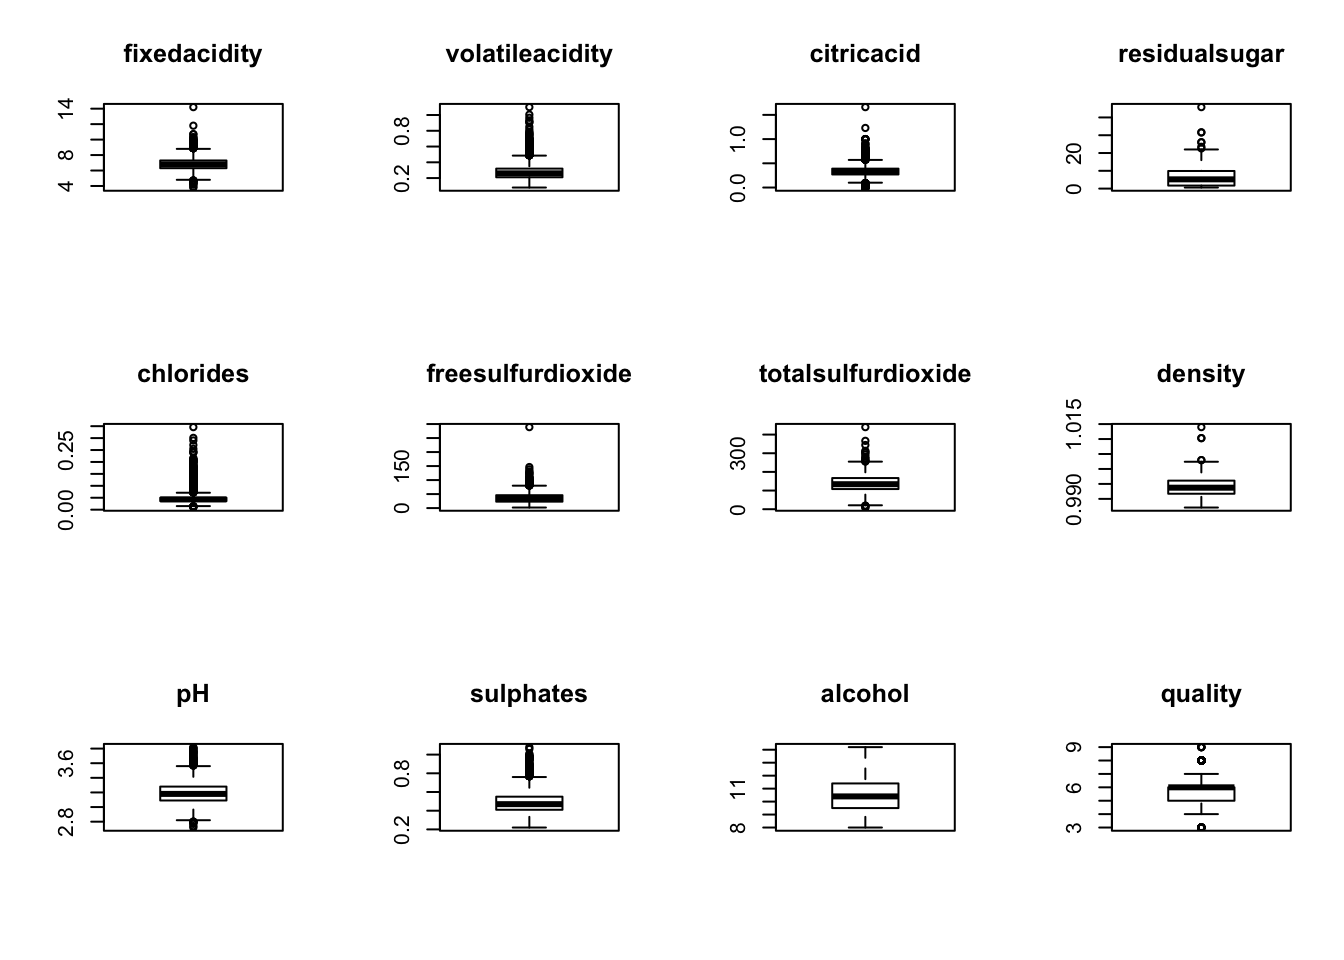
\includegraphics{Trabalho_Estatistica_180908_files/figure-latex/unnamed-chunk-17-1.pdf}

Análise:

Todos os Box Plots dos vinhos brancos apresentarem Outliers (exceto a
variavel alcohol), que pode ser efeito dos tamanhos de amostra, os
BoxPlots com maiores quantidade de outliers são: volatileacidity,
citricacid, chlorides, freesulfurdioxide, citricacid e freesulfurdioxide
com valores pontuais bem distantes da distribuição. Valeria uma melhor
avaliação destes pontos de medidas para verificação se realmente são
pontos fora da curva esperada.

Distribuições assimetricas, com principal atenção para residualsugar,
onde a assimentria se destaca na forma da caixa de dos bigodes do Box
Plot. Mediana deslocada para o Q1 e bigode inferior bem menor que o
superior.

\begin{Shaded}
\begin{Highlighting}[]
\KeywordTok{boxplot.stats}\NormalTok{(white}\OperatorTok{$}\NormalTok{residualsugar)}
\end{Highlighting}
\end{Shaded}

\begin{verbatim}
## $stats
## [1]  0.6  1.7  5.2  9.9 22.0
## 
## $n
## [1] 4898
## 
## $conf
## [1] 5.014877 5.385123
## 
## $out
## [1] 26.05 31.60 22.60 45.80 31.60 26.05 23.50
\end{verbatim}

\begin{Shaded}
\begin{Highlighting}[]
\NormalTok{AIQ_residualsugar<-}\KeywordTok{quantile}\NormalTok{(white}\OperatorTok{$}\NormalTok{residualsugar,.}\DecValTok{75}\NormalTok{,}\DataTypeTok{type=}\DecValTok{2}\NormalTok{)}\OperatorTok{-}\KeywordTok{quantile}\NormalTok{(white}\OperatorTok{$}\NormalTok{residualsugar,.}\DecValTok{25}\NormalTok{,}\DataTypeTok{type=}\DecValTok{2}\NormalTok{)}
\NormalTok{AIQ_residualsugar}
\end{Highlighting}
\end{Shaded}

\begin{verbatim}
## 75% 
## 8.2
\end{verbatim}

\begin{Shaded}
\begin{Highlighting}[]
\NormalTok{limsup_residualsugar=}\StringTok{ }\KeywordTok{quantile}\NormalTok{(white}\OperatorTok{$}\NormalTok{residualsugar,.}\DecValTok{75}\NormalTok{,}\DataTypeTok{type=}\DecValTok{4}\NormalTok{)}\OperatorTok{+}\FloatTok{1.5}\OperatorTok{*}\NormalTok{AIQ_residualsugar}
\NormalTok{limsup_residualsugar}
\end{Highlighting}
\end{Shaded}

\begin{verbatim}
##  75% 
## 22.2
\end{verbatim}

\begin{Shaded}
\begin{Highlighting}[]
\NormalTok{liminf_residualsugar=}\StringTok{ }\KeywordTok{quantile}\NormalTok{(white}\OperatorTok{$}\NormalTok{residualsugar,.}\DecValTok{25}\NormalTok{,}\DataTypeTok{type=}\DecValTok{2}\NormalTok{)}\OperatorTok{-}\FloatTok{1.5}\OperatorTok{*}\NormalTok{AIQ_residualsugar}
\NormalTok{liminf_residualsugar}
\end{Highlighting}
\end{Shaded}

\begin{verbatim}
##   25% 
## -10.6
\end{verbatim}

Análise:

Sobre as estatísticas do BoxPlot (boxplot.stat) podemos dizer: - O
bigode inferiro = valor mínimo (0,6), os qurtis Q1 = 1,7 e Q2 (mediana)
= 5,2 e Q3 = 9,9. O bigode superior = 22,0. Como temos valores maiores
que o 22,0, teremos outliers acima de 22,0. Mostrado no \$out. - Os
valores do \$conf, são (segundo Chambers e McGill) aproximadamente o
intervalo de confiança para a mediana.

Temos também a amplitude entre quartis: Q3 - Q1 = 8,2

\begin{Shaded}
\begin{Highlighting}[]
\CommentTok{#excluir outliers}

\KeywordTok{plot}\NormalTok{(quality}\OperatorTok{~}\NormalTok{residualsugar)}
\end{Highlighting}
\end{Shaded}

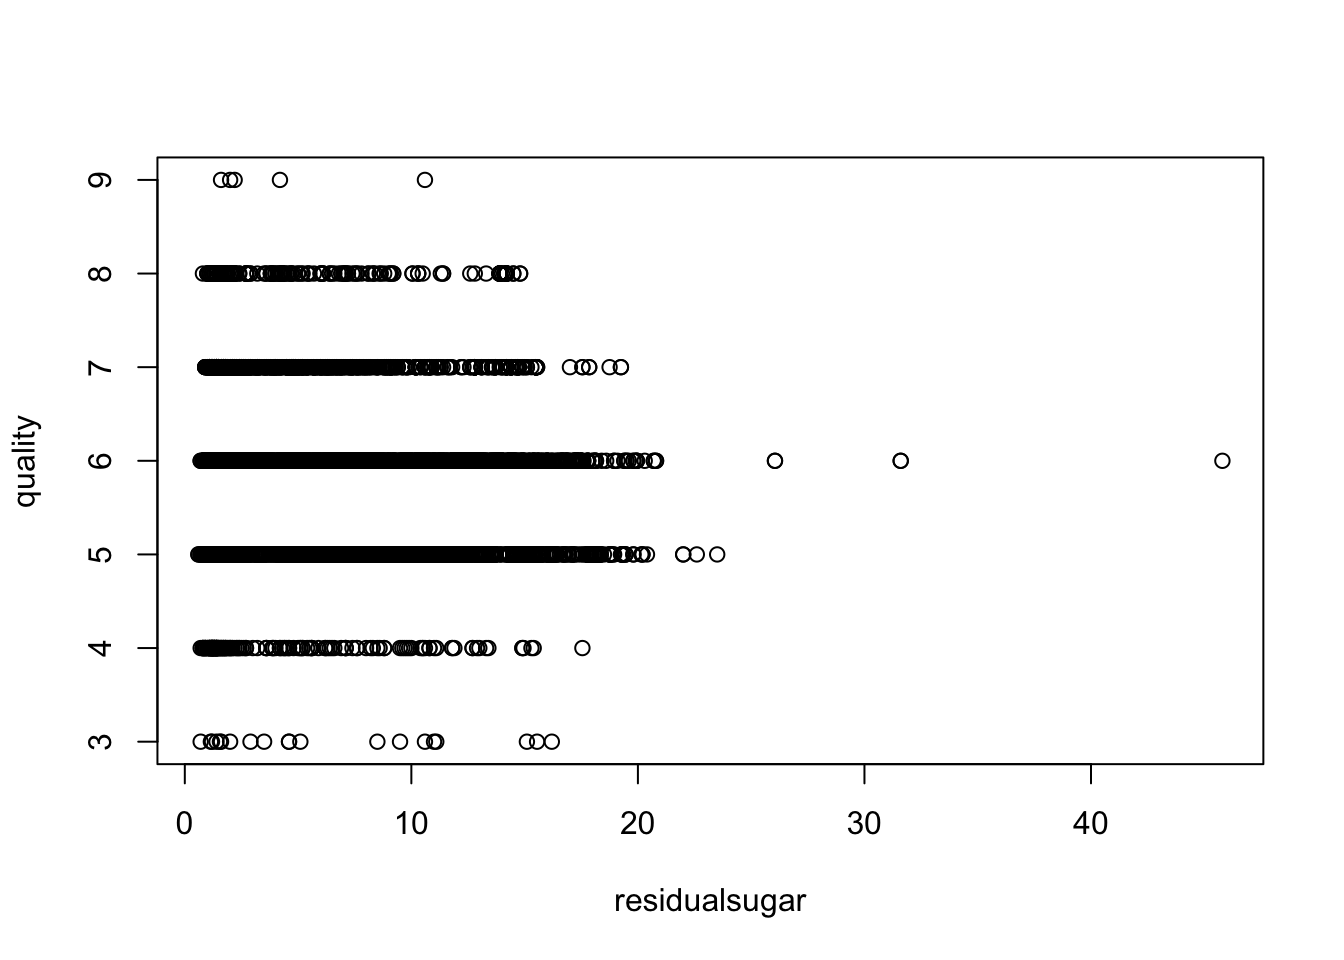
\includegraphics{Trabalho_Estatistica_180908_files/figure-latex/unnamed-chunk-19-1.pdf}

\begin{Shaded}
\begin{Highlighting}[]
\NormalTok{white1<-}\KeywordTok{subset}\NormalTok{(white, residualsugar}\OperatorTok{<=}\FloatTok{22.2}\NormalTok{)   }

\CommentTok{#fix(white1)}
\end{Highlighting}
\end{Shaded}

Análise:

Analisando o gráfico do residuo de açucar (resildualsugar) x nota de
qualidade dos vinhos brancos (quality), podemos perceber uma maior
concentração de resíduos de açucar para os vinhos com notas entre 5 e 6

\begin{Shaded}
\begin{Highlighting}[]
\KeywordTok{attach}\NormalTok{(white1)}
\end{Highlighting}
\end{Shaded}

\begin{verbatim}
## The following objects are masked from white:
## 
##     alcohol, chlorides, citricacid, density, fixedacidity,
##     freesulfurdioxide, pH, quality, residualsugar, sulphates,
##     totalsulfurdioxide, volatileacidity
\end{verbatim}

\begin{verbatim}
## The following objects are masked from Vinhos (pos = 5):
## 
##     alcohol, chlorides, citricacid, density, fixedacidity,
##     freesulfurdioxide, pH, quality, residualsugar, sulphates,
##     totalsulfurdioxide, volatileacidity
\end{verbatim}

\begin{verbatim}
## The following objects are masked from Vinhos (pos = 6):
## 
##     alcohol, chlorides, citricacid, density, fixedacidity,
##     freesulfurdioxide, pH, quality, residualsugar, sulphates,
##     totalsulfurdioxide, volatileacidity
\end{verbatim}

\begin{verbatim}
## The following objects are masked from Vinhos (pos = 7):
## 
##     alcohol, chlorides, citricacid, density, fixedacidity,
##     freesulfurdioxide, pH, quality, residualsugar, sulphates,
##     totalsulfurdioxide, volatileacidity
\end{verbatim}

\begin{verbatim}
## The following objects are masked from Vinhos (pos = 9):
## 
##     alcohol, chlorides, citricacid, density, fixedacidity,
##     freesulfurdioxide, pH, quality, residualsugar, sulphates,
##     totalsulfurdioxide, volatileacidity
\end{verbatim}

\begin{Shaded}
\begin{Highlighting}[]
\KeywordTok{summary}\NormalTok{(white1)}
\end{Highlighting}
\end{Shaded}

\begin{verbatim}
##     quality       fixedacidity    volatileacidity   citricacid    
##  Min.   :3.000   Min.   : 3.800   Min.   :0.080   Min.   :0.0000  
##  1st Qu.:5.000   1st Qu.: 6.300   1st Qu.:0.210   1st Qu.:0.2700  
##  Median :6.000   Median : 6.800   Median :0.260   Median :0.3200  
##  Mean   :5.878   Mean   : 6.854   Mean   :0.278   Mean   :0.3341  
##  3rd Qu.:6.000   3rd Qu.: 7.300   3rd Qu.:0.320   3rd Qu.:0.3900  
##  Max.   :9.000   Max.   :14.200   Max.   :1.100   Max.   :1.6600  
##  residualsugar      chlorides       freesulfurdioxide totalsulfurdioxide
##  Min.   : 0.600   Min.   :0.00900   Min.   :  2.00    Min.   :  9.0     
##  1st Qu.: 1.700   1st Qu.:0.03600   1st Qu.: 23.00    1st Qu.:108.0     
##  Median : 5.200   Median :0.04300   Median : 34.00    Median :134.0     
##  Mean   : 6.354   Mean   :0.04575   Mean   : 35.31    Mean   :138.3     
##  3rd Qu.: 9.850   3rd Qu.:0.05000   3rd Qu.: 46.00    3rd Qu.:167.0     
##  Max.   :22.000   Max.   :0.34600   Max.   :289.00    Max.   :440.0     
##     density             pH          sulphates         alcohol     
##  Min.   :0.9871   Min.   :2.720   Min.   :0.2200   Min.   : 8.00  
##  1st Qu.:0.9917   1st Qu.:3.090   1st Qu.:0.4100   1st Qu.: 9.50  
##  Median :0.9937   Median :3.180   Median :0.4700   Median :10.40  
##  Mean   :0.9940   Mean   :3.188   Mean   :0.4899   Mean   :10.51  
##  3rd Qu.:0.9961   3rd Qu.:3.280   3rd Qu.:0.5500   3rd Qu.:11.40  
##  Max.   :1.0024   Max.   :3.820   Max.   :1.0800   Max.   :14.20
\end{verbatim}

\begin{Shaded}
\begin{Highlighting}[]
\KeywordTok{plot}\NormalTok{(residualsugar,alcohol)}
\KeywordTok{abline}\NormalTok{(}\DataTypeTok{v=}\KeywordTok{mean}\NormalTok{(residualsugar), }\DataTypeTok{col=}\StringTok{"red"}\NormalTok{)}
\KeywordTok{abline}\NormalTok{(}\DataTypeTok{h=}\KeywordTok{mean}\NormalTok{(alcohol), }\DataTypeTok{col=}\StringTok{"green"}\NormalTok{)}
\end{Highlighting}
\end{Shaded}

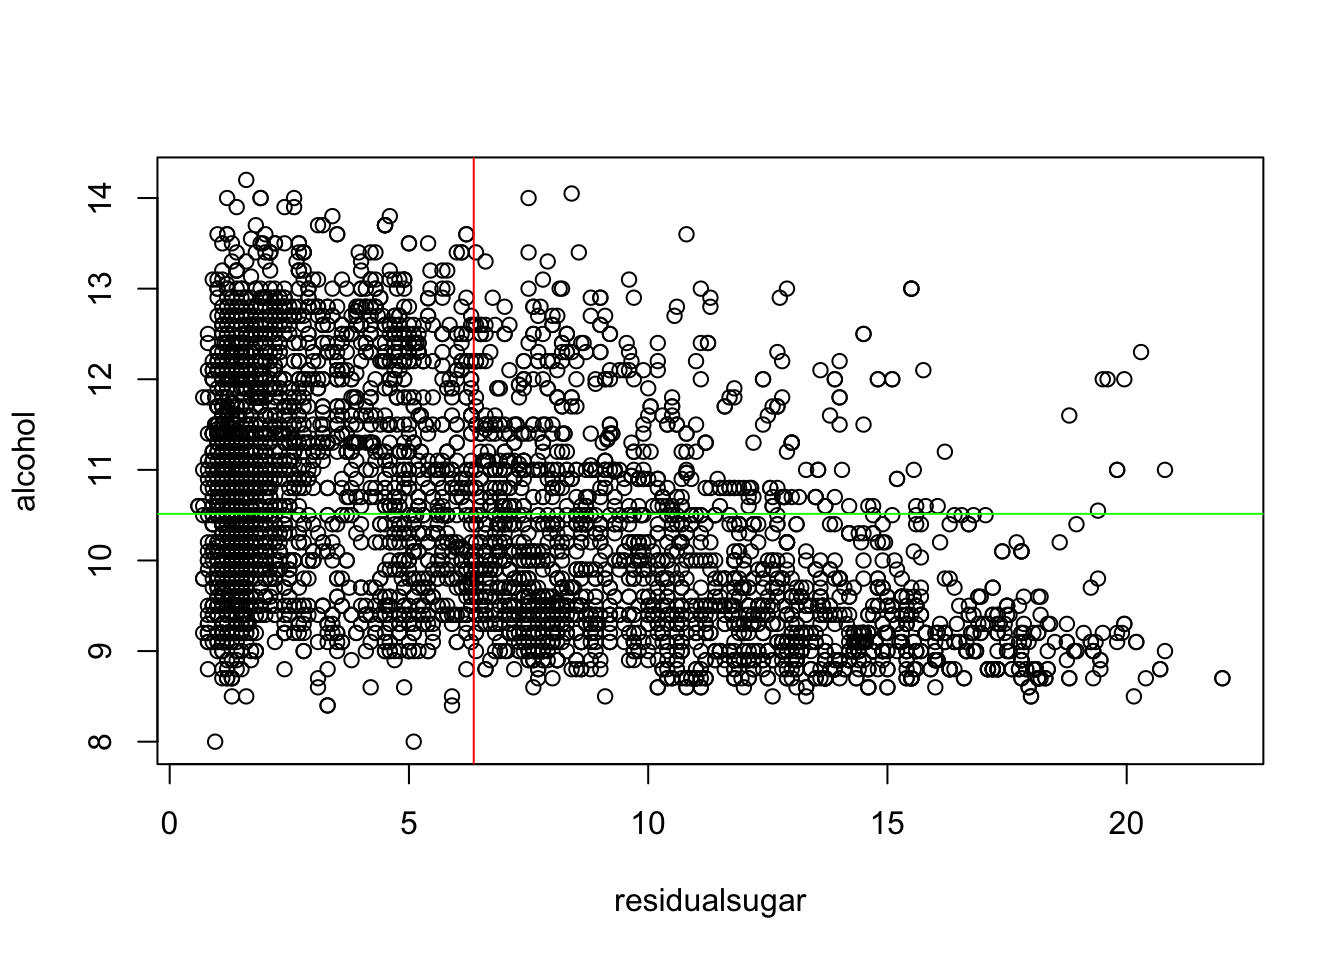
\includegraphics{Trabalho_Estatistica_180908_files/figure-latex/unnamed-chunk-20-1.pdf}

Análise:

Após tirarmos o valor de residualsugar acima de 22,2 (limite do bigode
do BoxPlot), podemos analisar que existe uma correlação negativa entre
as variáveis, ou seja quanto maior o teor alcolico, menor a concentração
de resíduo de açucar, com exceção de valores de baixo resíduo de açucar
e baixa quantidade de alcool, que possivelmente pode ser explicado por
não ter açucar suficiente no início do processo (suco de uva) e que não
provoca uma fermentação que eleve o nível de alcool no vinho.

Ainda observando que estes valores de residuo de açucar baixo e alcool
baixo, reduzem os valores de média para as duas variáveis, podendo
enviezar a interpretação de uma futura análise de regressão.

\begin{Shaded}
\begin{Highlighting}[]
\CommentTok{# matriz de correlaÁıes}
\NormalTok{matcor <-}\StringTok{ }\KeywordTok{cor}\NormalTok{(white1)}
\KeywordTok{print}\NormalTok{(matcor, }\DataTypeTok{digits =} \DecValTok{2}\NormalTok{)}
\end{Highlighting}
\end{Shaded}

\begin{verbatim}
##                    quality fixedacidity volatileacidity citricacid
## quality             1.0000       -0.114         -0.1963    -0.0088
## fixedacidity       -0.1141        1.000         -0.0248     0.2895
## volatileacidity    -0.1963       -0.025          1.0000    -0.1529
## citricacid         -0.0088        0.290         -0.1529     1.0000
## residualsugar      -0.0995        0.087          0.0460     0.0914
## chlorides          -0.2095        0.023          0.0700     0.1132
## freesulfurdioxide   0.0088       -0.049         -0.0949     0.0943
## totalsulfurdioxide -0.1746        0.091          0.0892     0.1207
## density            -0.3176        0.268          0.0032     0.1483
## pH                  0.0991       -0.427         -0.0334    -0.1643
## sulphates           0.0535       -0.017         -0.0379     0.0616
## alcohol             0.4363       -0.120          0.0673    -0.0765
##                    residualsugar chlorides freesulfurdioxide
## quality                   -0.100    -0.210           0.00876
## fixedacidity               0.087     0.023          -0.04884
## volatileacidity            0.046     0.070          -0.09485
## citricacid                 0.091     0.113           0.09425
## residualsugar              1.000     0.086           0.30987
## chlorides                  0.086     1.000           0.10095
## freesulfurdioxide          0.310     0.101           1.00000
## totalsulfurdioxide         0.408     0.199           0.61591
## density                    0.831     0.261           0.30898
## pH                        -0.199    -0.091           0.00018
## sulphates                 -0.028     0.017           0.06009
## alcohol                   -0.462    -0.362          -0.25022
##                    totalsulfurdioxide density       pH sulphates alcohol
## quality                       -0.1746 -0.3176  0.09913     0.053   0.436
## fixedacidity                   0.0905  0.2682 -0.42667    -0.017  -0.120
## volatileacidity                0.0892  0.0032 -0.03342    -0.038   0.067
## citricacid                     0.1207  0.1483 -0.16430     0.062  -0.077
## residualsugar                  0.4081  0.8315 -0.19916    -0.028  -0.462
## chlorides                      0.1990  0.2613 -0.09063     0.017  -0.362
## freesulfurdioxide              0.6159  0.3090  0.00018     0.060  -0.250
## totalsulfurdioxide             1.0000  0.5436  0.00274     0.135  -0.448
## density                        0.5436  1.0000 -0.09845     0.075  -0.806
## pH                             0.0027 -0.0984  1.00000     0.155   0.121
## sulphates                      0.1348  0.0748  0.15517     1.000  -0.018
## alcohol                       -0.4484 -0.8064  0.12103    -0.018   1.000
\end{verbatim}

Análise:

Observando as correlações, algumas nos chamam a atenção: - residualsugar
x density = 0,8315, que comprova que vinhos com muito açucar tem maior
densidade, no sentido inverso; - vinhos com muito alcool tem menor
densidade (correlação = -0,8064). - forte correlação entre
freesulfurdioxide x totalsulfurdioxide (0,61591), devido ao livre fazer
parte do total deste conservante.

\begin{Shaded}
\begin{Highlighting}[]
\CommentTok{#library(corrgram)}
\CommentTok{#corrgram(matcor, type = "cor", lower.panel = panel.shade, upper.panel = panel.pie)}

\NormalTok{panel.cor <-}\StringTok{ }\ControlFlowTok{function}\NormalTok{(x, y, }\DataTypeTok{digits=}\DecValTok{2}\NormalTok{, }\DataTypeTok{prefix =}\StringTok{""}\NormalTok{, cex.cor,}
\NormalTok{                      ...)  \{}
\NormalTok{  usr <-}\StringTok{ }\KeywordTok{par}\NormalTok{(}\StringTok{"usr"}\NormalTok{)}
  \KeywordTok{on.exit}\NormalTok{(}\KeywordTok{par}\NormalTok{(usr))}
  \KeywordTok{par}\NormalTok{(}\DataTypeTok{usr =} \KeywordTok{c}\NormalTok{(}\DecValTok{0}\NormalTok{, }\DecValTok{1}\NormalTok{, }\DecValTok{0}\NormalTok{, }\DecValTok{1}\NormalTok{))}
\NormalTok{  r <-}\StringTok{ }\KeywordTok{cor}\NormalTok{(x, y , }\DataTypeTok{use =} \StringTok{"pairwise.complete.obs"}\NormalTok{)}
\NormalTok{  txt <-}\StringTok{ }\KeywordTok{format}\NormalTok{(}\KeywordTok{c}\NormalTok{(r, }\FloatTok{0.123456789}\NormalTok{), }\DataTypeTok{digits =}\NormalTok{ digits) [}\DecValTok{1}\NormalTok{]}
\NormalTok{  txt <-}\StringTok{ }\KeywordTok{paste}\NormalTok{(prefix, txt, }\DataTypeTok{sep =} \StringTok{""}\NormalTok{)}
  \ControlFlowTok{if}\NormalTok{ (}\KeywordTok{missing}\NormalTok{(cex.cor))}
\NormalTok{    cex <-}\StringTok{ }\FloatTok{0.8}\OperatorTok{/}\KeywordTok{strwidth}\NormalTok{(txt)}
  \CommentTok{# abs(r) È para que na saÌda as correlaÁıes ficam proporcionais}
  \KeywordTok{text}\NormalTok{(}\FloatTok{0.5}\NormalTok{, }\FloatTok{0.5}\NormalTok{, txt, }\DataTypeTok{cex =}\NormalTok{ cex }\OperatorTok{*}\StringTok{ }\KeywordTok{abs}\NormalTok{(r))}
\NormalTok{\}}
\CommentTok{#pdf(file = "grafico.pdf")}
\KeywordTok{pairs}\NormalTok{(white1, }\DataTypeTok{lower.panel=}\NormalTok{panel.smooth, }\DataTypeTok{upper.panel=}\NormalTok{panel.cor)}
\end{Highlighting}
\end{Shaded}

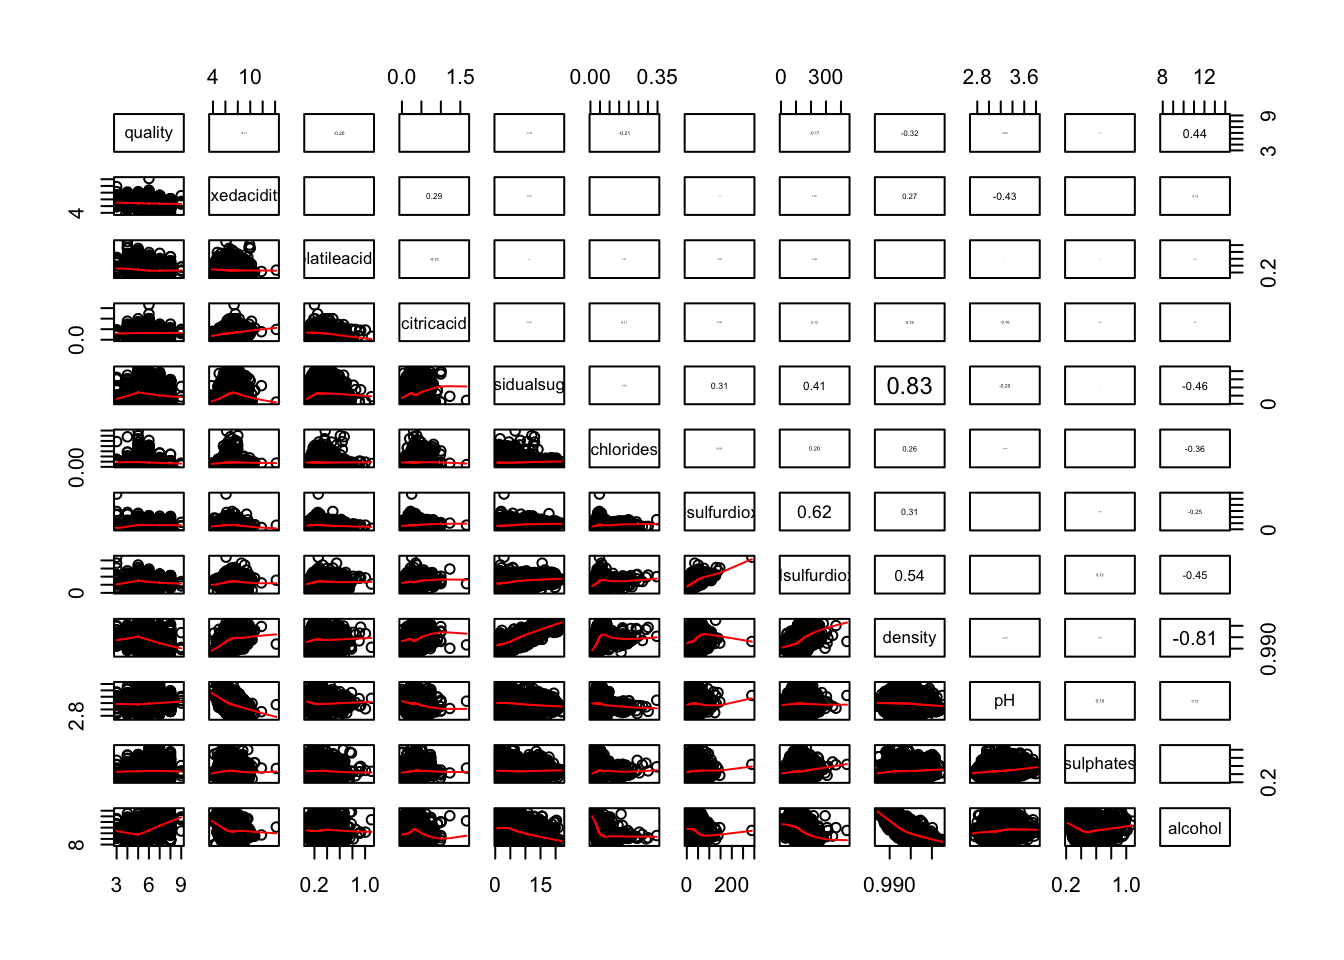
\includegraphics{Trabalho_Estatistica_180908_files/figure-latex/unnamed-chunk-22-1.pdf}

Análise:

Agora podemos comprovar atraves de gráficos o que já foi comentado a
análise da tabela de correlação


\end{document}
